%%%%%%% Document settings %%%%%%%%%%
\documentclass{DESSThesis}

%%%%%%%%%%% Additional Packages %%%%%%%%%%%%%%%%%%%%%%%%%%%
% Some suggestions are added, simply uncomment
%Highlight todos within text
% \usepackage[colorinlistoftodos,prependcaption, textsize=tiny]{todonotes} 
% \newcommandx{\note}[2][1=]{\todo[inline, size = \small, backgroundcolor=SeaGreen!25, bordercolor=PineGreen, #1]{#2}}
% \usepackage{algorithm} %Algorithm environment, requires texlive-science
% \usepackage{listings}
% \usepackage{algpseudocode} %Pseudocode commands used in algorithm
% \renewcommand{\algorithmicrequire}{\textbf{Input: }}
% \renewcommand{\algorithmicensure}{\textbf{Output: }}
\usepackage{multirow}
\usepackage{booktabs}
\usepackage[table]{xcolor}
\usepackage{enumitem}
\usepackage{tcolorbox}
\usepackage{listings}
\usepackage{makecell}
\usepackage{comment}

\definecolor{codegreen}{rgb}{0,0.6,0}
\definecolor{codegray}{rgb}{0.5,0.5,0.5}
\definecolor{codepurple}{rgb}{0.58,0,0.82}
\definecolor{backcolour}{rgb}{0.95,0.95,0.92}

\lstdefinestyle{mystyle}{
    backgroundcolor=\color{backcolour},   
    commentstyle=\color{codegreen},
    keywordstyle=\color{magenta},
    numberstyle=\tiny\color{codegray},
    stringstyle=\color{codepurple},
    basicstyle=\ttfamily\footnotesize,
    breakatwhitespace=false,         
    breaklines=true,                 
    captionpos=b,                    
    keepspaces=true,                 
    numbers=left,                    
    numbersep=5pt,                  
    showspaces=false,                
    showstringspaces=false,
    showtabs=false,                  
    tabsize=2
}

\lstset{style=mystyle}

%%%%%%%%%%% Personalized commands and definitions %%%%%%%%%
\newcommand{\bigO}[1]{\ensuremath{\mathcal{O}\big(#1\big)}}
\newtheorem*{theorem}{Theorem}
\DeclareMathOperator{\supp}{supp} %prevents mathmode to change the font
%Plot own functions using tikz and pgfplot
\pgfplotsset{compat=1.13}
\pgfmathdeclarefunction{gauss}{2}{%
  \pgfmathparse{1/(#2*sqrt(2*pi))*exp(-((x-#1)^2)/(2*#2^2))}%
}

%%%%%%%%%%%%%%%%%%%%%% Hyphenations %%%%%%%%%%%%%%
\hyphenation{trac-ta-ble}

%%%%%%%%%%%%%%%%%%%%%%%%%%%%%%%%%%%%%%%%%%%%%%%%%%

\overfullrule=2cm %Show hboxes incase of misalignment, uncomment before handing in!

\bibliography{references}

\begin{document}

%%%%%%%%%%%%%%%%%%%%% Frontpage %%%%%%%%%%%%%%%%%%%%%%%%%%%%%%% 
\def \TypeofThesis{Master's Thesis}
\def \TitleofThesis{Something Interesting and Meaningful}
\def \AuthorofThesis{Your Name}
\def \Supervisor{Your Supervisor/Examiner} % typically Prof. Dr. Markus Strohmaier
\def \Advisor{Your Advisor}
%%%%%%%%%%%%%%%%%%%%%%%%%%%%%%%%%%%%%%%%%
% Academic Title Page
% LaTeX Template
% Version 2.0 (17/7/17)
%
% This template was downloaded from:
% http://www.LaTeXTemplates.com
%
% Original author:
% WikiBooks (LaTeX - Title Creation) with modifications by:
% Vel (vel@latextemplates.com)
% Lorena Reintgen
%
% License:
% CC BY-NC-SA 3.0 (http://creativecommons.org/licenses/by-nc-sa/3.0/)
% 
%
%%%%%%%%%%%%%%%%%%%%%%%%%%%%%%%%%%%%%%%%%

%----------------------------------------------------------------------------------------
% TITLE PAGE
%----------------------------------------------------------------------------------------

\begin{titlepage} % Suppresses displaying the page number on the title page and the subsequent page counts as page 1
\newcommand{\HRule}{\rule{\linewidth}{0.5mm}} % Defines a new command for horizontal lines, change thickness here
\center % Centre everything on the page
%\renewcommand{\baselinestretch}{1.2} %vertical spacing between lines
%------------------------------------------------
%  Headings
%------------------------------------------------
\textsc{\LARGE \TypeofThesis}\\[1.5cm] % Main heading such as the name of your university/college
%------------------------------------------------
%  Title
%------------------------------------------------
\HRule\\[0.4cm]
\linespread{1.7}\selectfont
{\huge\bfseries Adaptive Code Generation for the Analysis of
Donated Data with Large Language Models}\\ % Title of your document
\HRule\\[1.5cm]
\linespread{1.2}\selectfont
%------------------------------------------------
%  Author(s)
%------------------------------------------------
    \vfill
    \textit{\large submitted by}\\[0.5cm] % Major heading
\textsc{\Large Miger Shkrepa}\\[0.5cm] % Minor heading
    \vfill

{\large\textit{Submitted to the}}\\
\Large Chair of Data Science in the Economic and Social Sciences \\
    {\large\textit{within the}}\\
    Faculty of Business Administration \\
    at the University of Mannheim
    
    %------------------------------------------------
%  Date
%------------------------------------------------
\vfill\vfill\vfill % Position the date 3/4 down the remaining page
{\large September 22, 2025} % Date, change the \today to a set date if you want to be precise

\vfill\vfill\vfill
{ \large \center 
\textit{Advisor:}\\
Maximilian Kreutner, PhD
}

\vfill
{ \large \center 
\textit{Supervisor:}\\
Prof. Dr. Markus Strohmaier 
}


%------------------------------------------------
%  Logo
%------------------------------------------------
%\vfill\vfill
%\includegraphics[width=0.2\textwidth]{placeholder.jpg}\\[1cm] % Include a department/university logo - this will require the graphicx package
 
%----------------------------------------------------------------------------------------
\vfill % Push the date up 1/4 of the remaining page
\end{titlepage}

%\vfill
\cleardoublepage

\newpage
\paragraph{Declaration of Authorship}\mbox{}\\

\noindent I hereby declare that the paper presented is my own work and that I have not called upon the help of a third party. In addition, I declare that neither I nor anybody else has submitted this paper or parts of it to obtain credits elsewhere before. I have clearly marked and acknowledged all quotations or references that have been taken from the works of others. All secondary literature and other sources are marked and listed in the bibliography. The same applies to all charts, diagrams and illustrations as well as to all internet resources. Moreover, I consent to my paper being electronically stored and sent anonymously in order to be checked for plagiarism. I am aware that if this declaration is not made, the paper may not be graded.

\vspace{4em}
\noindent Mannheim, September 22, 2025 \hfill\rule{5cm}{0.4pt} \\

\cleardoublepage

\newpage
\begin{abstract}
\mbox{}\\
\noindent The release and advancements of Large Language Models (LLMs) have significantly enhanced automation and efficiency in many tasks. Retrieval-Augmented Generation is set to improve the performance of these models even further by incorporating external knowledge to reduce hallucination in their responses. In this thesis, we propose leveraging the two technologies to reduce the need for manual updates in data analysis tools, particularly for donated data that is often provided in structurally changing packages. We analyze the performance of Llama3.1 8B, Codestral 22B, Qwen2.5 Coder 32B, Llama3.1 70B, Qwen2.5 72B, and Mistral Large Instruct across 13 Instagram data packages under various experimental setups, focusing on accuracy, error patterns, and code generation behavior. We find that for this task, knowledge augmentation produces poor results. As an approach, it is very prone to errors, with models frequently generating faulty file paths. When conducting similar experiments on a prompt-only setup, the performance is better in comparison, but still unsatisfactory, as the models still make frequent errors when processing or extracting data. Further analysis reveals that some of these shortcomings stem from the overly complex structure of the evaluated data packages and how Instagram structures them. When explicit instructions for navigating the data are introduced, the models reach superior results. However, since such instructions are also subject to updates in response to structural changes, we observe that the manual updating this research sought to remove is essential for achieving better performance. Nevertheless, a data researcher without programming skills but with knowledge of the donated data's structure can still leverage LLMs to automate processes by generating code. This work contributes to understanding the feasibility of using LLMs as an alternative to traditional manually maintained data analysis tools.
\end{abstract}

\cleardoublepage

\newpage
\paragraph{Acknowledgements}\mbox{}\\

\noindent I would like to express my gratitude to my advisor, Maximilian Kreutner, for his constant support and guidance throughout my thesis. I gratefully acknowledge the KISSKI project and Chat AI platform at GWDG for providing me with the resources necessary to conduct my experiments. I would also like to express my sincere gratitude to everyone who shared their personal data in support of this research.

Finally, I would like to thank my friends, family, and loved ones for their endless support, time, and everything they have dedicated to me.

\cleardoublepage

\tableofcontents

\listoftables

\listoffigures
%%%%%%%%%%%%%%%%%%%%% Abstract %%%%%%%%%%%%%%%%%%%%%%%%%%%%% 
\cleardoublepage
\pagenumbering{arabic} %pagenumbering always resets the page number
%%%%%%%%%%%%%%%%%%%%% Chapter 1 %%%%%%%%%%%%%%%%%%%%%% 

\chapter{Introduction}
\thispagestyle{empty}
With the incorporation of several digital tools and technologies in our daily lives, digital footprints of individuals are continuously generated and recorded. Social media, for instance, has enabled the shift of conversations and communication to online mediums, allowing for interactions across platforms such as Twitter, Facebook, Instagram, and others on a massive scale~\cite{IndiraSen2021ApplyingAT}. These platforms have become important spaces for civic participation, supporting emancipatory and transformative forms of individual engagement~\cite{doi:10.1177/2057047316683200}(see Figure~\ref{fig:networks_and_sources}). The digital documentation of basic everyday activities such as e-mail history, credit card transactions, and cell phone records has become normalized and often facilitates the efficiencies of modern life. Furthermore, informational objects that predate computers can now be easily scanned and converted into manipulable digital formats as well~\cite{annurev:/content/journals/10.1146/annurev-soc-060116-053457}. The scope of this widespread digitization is enhanced by the constant archiving of human behavior combined with the exponential growth of computational power~\cite{annurev:/content/journals/10.1146/annurev-soc-060116-053457}. The sheer volume of human data generated daily, and these examples represent only the tip of the digital data landscape.

\begin{figure}[htb!]
	\centering
	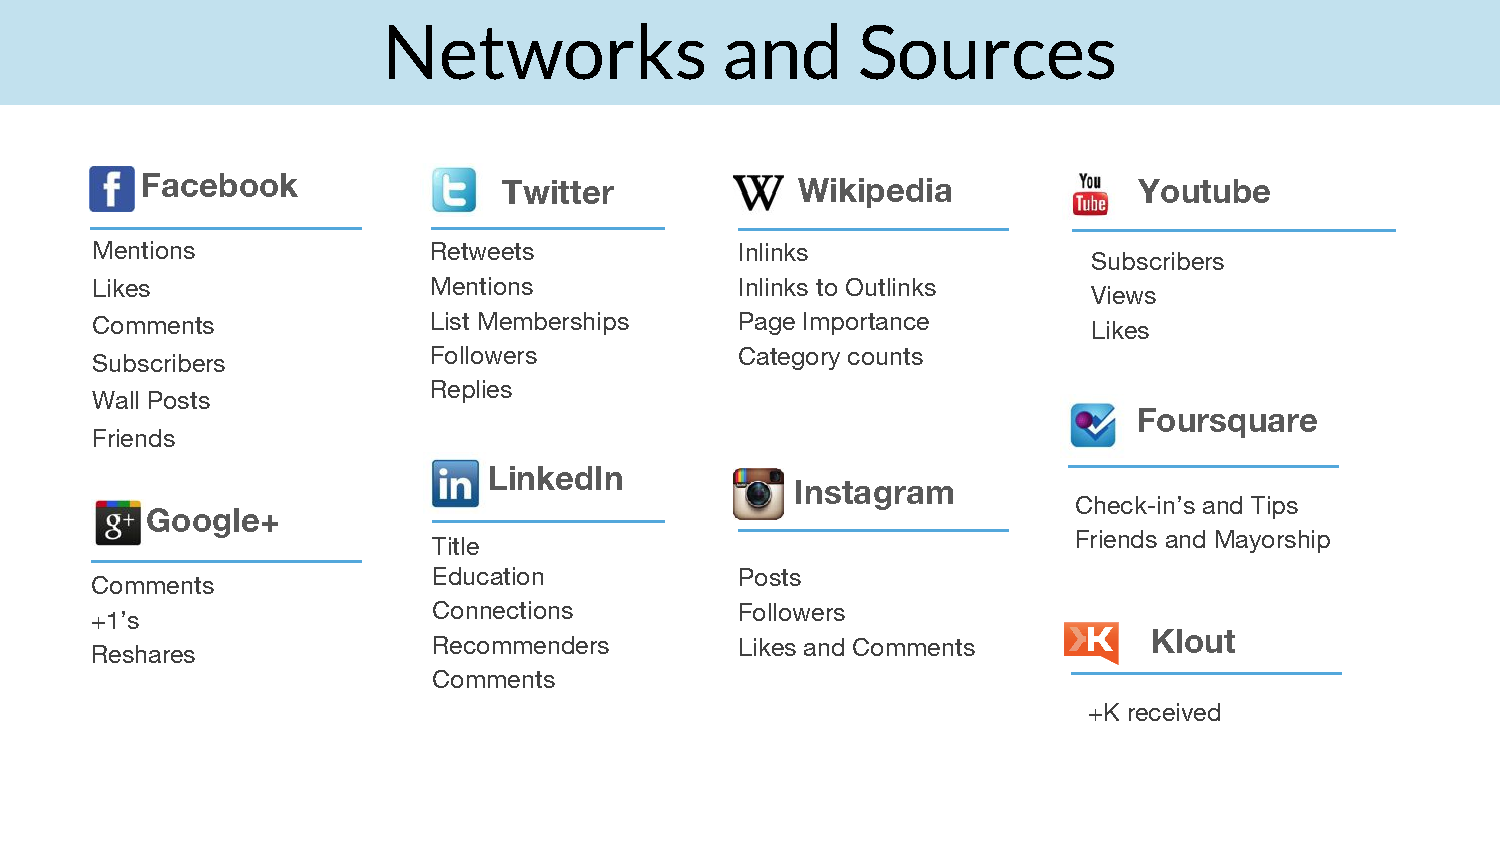
\includegraphics[width=0.9\linewidth]{img/Introduction/networks_and_sources.pdf}
	\caption[Social media networks and data sources]{\textbf{Social media networks and data sources}. Figure taken from~\cite{Rao_2016}. This image shows several social media platforms and only a subset of the data they collect that is generated from a user's active participation.}
	\label{fig:networks_and_sources}
\end{figure}

\paragraph{Digital Traces}\mbox{}\\

\noindent In this media-saturated world, people are constantly producing digital footprints, whether intentionally by active interaction or unintentionally through passive participation~\cite{doi:10.1177/20539517231213827,IJoC8650}. Digital traces are defined as numerically produced correlations of disparate kinds of data generated by human interactions in digital environments~\cite{IJoC8650}. These traces are created from a combination of technical and social processes. As such, these platforms serve as a treasure trove of data that can be leveraged across various studies~\cite{IndiraSen2021ApplyingAT}. They can help in evaluating, testing, and conceptualizing human behavior theories, especially those tied to the digital aspect of everyday life~\cite{IndiraSen2021ApplyingAT}. These digital trace data are geographically far-reaching and generated on a nearly continuous basis, providing unique insights into patterns of interaction and self-expression. The fine-grained nature of this data, coupled with the ability to collect large quantities in relatively short time frames, provides researchers with the opportunities to study a wide range of social and behavioral phenomena~\cite{Cesare_Lee_McCormick_Spiro_Zagheni_2018,Keusch_Kreuter_2021}. As a result, digital traces complement traditional research methods by providing large-scale and real-world data, capturing everyday behavior, and serving as a potential data source for psychological research~\cite{doi:10.1177/0963721419861410}.

Accessing this data by normal means is a rather difficult process as they are either blocked off in proprietary archives or can only be reached through restricted and opaque \emph{Application Programming Interfaces} (APIs)~\cite{Boeschoten2023}. Legal frameworks such as The General Data Protection and Regulation~\cite{europeanParliament2016a} help in mitigating these issues by granting people the right to access their recorded personal data. In accordance with this legislation, data collecting and processing entities are required to provide individuals with a digital copy of their personal data upon request. These digital copies are issued in the form of \emph{Data Download Packages} (DDPs) and facilitate numerous studies in detail. For instance, the open source tool Port~\cite{Boeschoten2023} provides researchers with the ability to customize data donation studies with the focus on DDPs.

\paragraph{DDPs and Challenges Associated with Them}\mbox{}\\

\noindent The continuously generated digital traces of individuals contribute directly to the creation of their DDPs. Digital trace data are generated in real time and are decentralized in nature, making them accessible to researchers from varied backgrounds~\cite{Cesare_Lee_McCormick_Spiro_Zagheni_2018}. However, they also present logistical challenges in terms of management and analysis. Effectively handling these characteristics calls for collaboration between researchers and those equipped with the technical expertise to analyze and visualize the data patterns~\cite{Cesare_Lee_McCormick_Spiro_Zagheni_2018}.

A key consideration is the resources necessary to collect digital trace data. These include the technical infrastructure for access (e.g., API fees), the development of research software and tools, lawful storage in compliance with regulations like the GDPR, and the computational resources for processing and analysis. Figure~\ref{fig:data_donation_overview} illustrates an overview of conducting such studies, from data acquisition to processing. Especially in data donation studies, additional challenges arise from the often unstable and poorly documented structure of DDPs~\cite{Ohme_Araujo_Boeschoten_Freelon_Ram_Reeves_Robinson_2024}. Advances in data integration, informatics, computational power, and data science are crucial to manage this volume of data~\cite{doi:10.1161/CIRCOUTCOMES.123.010150}.

\begin{figure}[htb!]
	\centering
	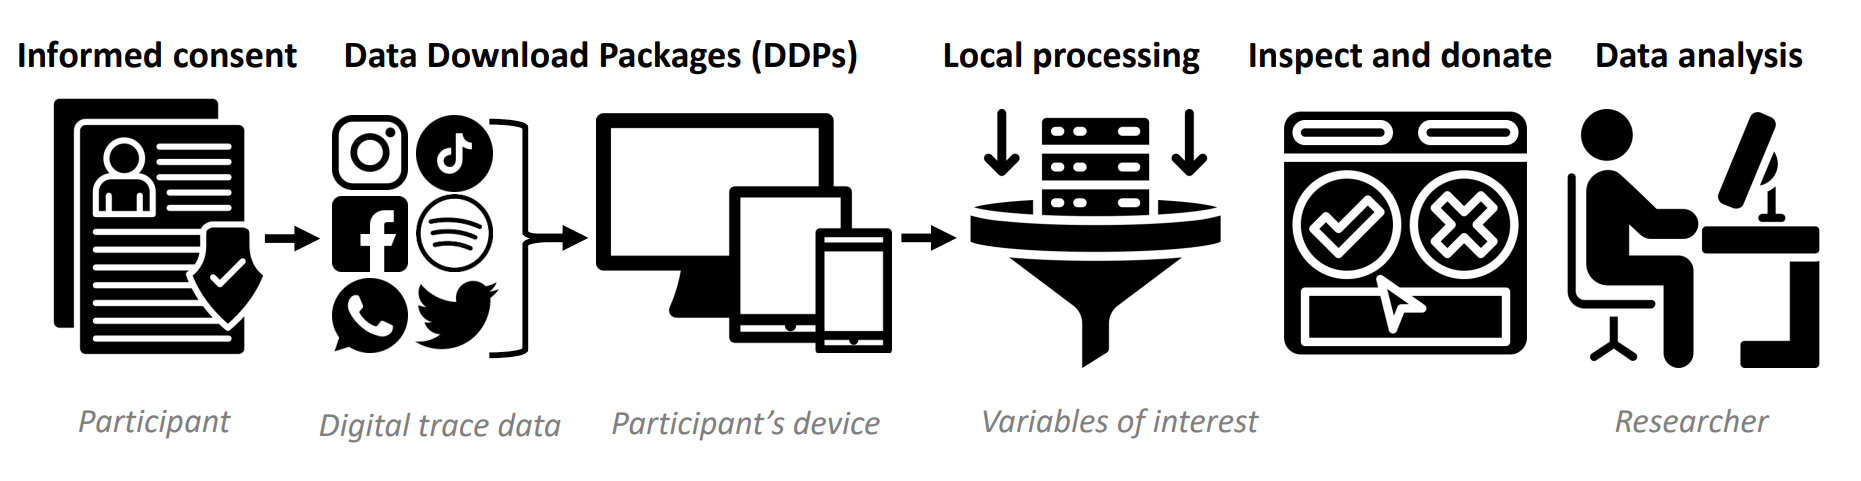
\includegraphics[width=0.9\linewidth]{img/Introduction/data_donation_overview.png}
	\caption[An overview of the participant's data donation flow]{\textbf{An overview of the participant's data donation flow}. Figure taken from~\cite{Boeschoten2023}. The process begins with participants requesting their DDPs from data collecting platforms, in accordance with GDPR. After downloading the DDP to their device, local processing offered by researcher-provided software extracts only the data relevant to the study. Participants then review the extracted data and, if they consent, the selected information is securely donated and made accessible for research analysis~\cite{Boeschoten2023}.}
	\label{fig:data_donation_overview}
\end{figure}

Since DDPs are recorded by several data controllers across different platforms, they can vary greatly in structure and content~\cite{boeschoten2021automatic}. These packages may contain a wide array of formats for media files (PNG, JPG, MP4, HTML) and text files (JSON, HTML, TXT, OPUS). These structural differences may even occur in DDPs issued by the same controller for the same platform, driven by the introduction of new features, obsolescence of some functionalities, and due to some data being maintained only periodically. As a result, researchers are forced to modify their developed tools to accommodate for these changes and avoid deprecation.

\section{Research Objective} \label{research_objective}

To address these challenges, in this paper, we propose leveraging \emph{Large Language Models} (LLMs) and incorporating \emph{Retrieval-Augmented Generation} (RAG)~\cite{lewis2020retrieval} to dynamically generate code that attempts to answer data-specific queries. Instead of manually updating data donation tools in response to evolving DDP structures, LLMs can generate scripts that extract relevant information based on contextual details regarding the data structure of the provided DDPs. This approach offers an alternative to researchers by allowing them to automate data processing while reducing dependency on fixed data formats and providing adaptability and flexibility in handling diverse and structure-updating datasets.

This thesis aims to develop and evaluate a novel approach that leverages LLMs to generate code for answering data-specific queries based on information regarding individuals' DDPs. The core objective of this study is to assess the feasibility and effectiveness of these models in understanding the data structure and associating its content with the user-provided question. In addition, it examines the capabilities of LLM-generated code in automatically processing and extracting relevant data from these structured datasets while minimizing manual intervention. To guide this research, we formulate the following \emph{research questions} (RQs):

\begin{enumerate}
    \item[] \textbf{RQ1: Can LLMs accurately interpret the diverse data structures of DDPs?}
    
    \item[] \textbf{RQ2: How effectively can LLMs generate code to answer research questions based on user-specific data?}

    \item[] \textbf{RQ3: How does the LLMs' performance differ when contextual information is provided via prompts versus RAG?}

    \item[] \textbf{RQ4: What type of experimental and contextual input setup yields the best results in LLM-generated code for this specific task?}
\end{enumerate}

Firstly, we assess whether LLMs can generate code that accurately represents the complex structures of DDPs. Since DDPs vary in format and complexity, the models must correctly interpret their structure when responding, ensuring consistency with the actual data organization.

Secondly, we evaluate how effectively LLMs produce scripts that can answer data-specific queries. Beyond structural representation, the models must retrieve relevant information accurately, handle different queries, and attempt to refine responses through retries. 

Thirdly, we compare the results of using RAG versus prompt-only instructions when providing the structure of the DDPs as context for the model's code generation. This helps determine whether simply supplying the structural information through prompts can match or outdo the performance of more complex retrieval-based methods, and illustrate how each approach impacts usability and accuracy.

Lastly, we explore which kind of contextual and experimental setup offers the best performance in DDP data analysis code generation. Specifically, we compare different setups of providing the full scope of the DDP structure alongside offering only the structure of the relevant files involved. This experiment aims to identify which strategy yields the most reliable and efficient code outputs.

This research aims to bridge the gap between automated data processing and adaptive code generation. We investigate an alternative solution to traditional manually maintained data extraction tools. The findings could help researchers working with DDPs by automatically generating code to extract relevant data, reducing the need for manual script development and adaptation.

\section{Thesis Structure}

This thesis begins with an introduction to the topics and fundamentals of LLMs and RAG in Chapter~\ref{chap:LLM_and_RAG}. Chapter~\ref{chap:related_work} reviews related work in the domain of data analysis with LLMs and RAG, discussing their applications, general performance, and common limitations. Chapter~\ref{chap:methodology} describes the experimental setup, including details on the pipeline design, the models employed, and how they are accessed. It also outlines the evaluation schema and the domains it covers, as well as details on how each experiment is structured. Chapter~\ref{chap:results} presents the results of the conducted experiments, while Chapter~\ref{chap:discussion} provides an interpretation of these results, highlights limitations, and suggests directions for future research. Finally, Chapter~\ref{chap:conclusion} concludes by summarizing the experiments and the key insights gained.

\chapter{Large Language Models and RAG} \label{chap:LLM_and_RAG}

\emph{Language Models} (LMs) are considered as one of humanity's most potent tools~\cite{wang2024historydevelopmentprincipleslarge}. However, at their core, they remain mathematical models that generate outputs based on statistical distributions~\cite{10.1145/3624724}. Before delving further into the framework of this research, it is important to provide some generic knowledge on the key concepts behind LLMs, RAG architectures, and the development history that led to their emergence. The following sections provide a brief overview of these topics.

\section{History of Language Models}

LMs predict how likely a word is to appear based on the words and the contextual information around it. This capability makes them valuable tools in technologies such as speech recognition, machine translation, and natural language systems~\cite{lau1994adaptive}. To provide a better understanding of LMs, we go over their main developmental stages and their history, as summarized in Figure~\ref{fig:history}. 

\begin{figure}[H]
    \centering
    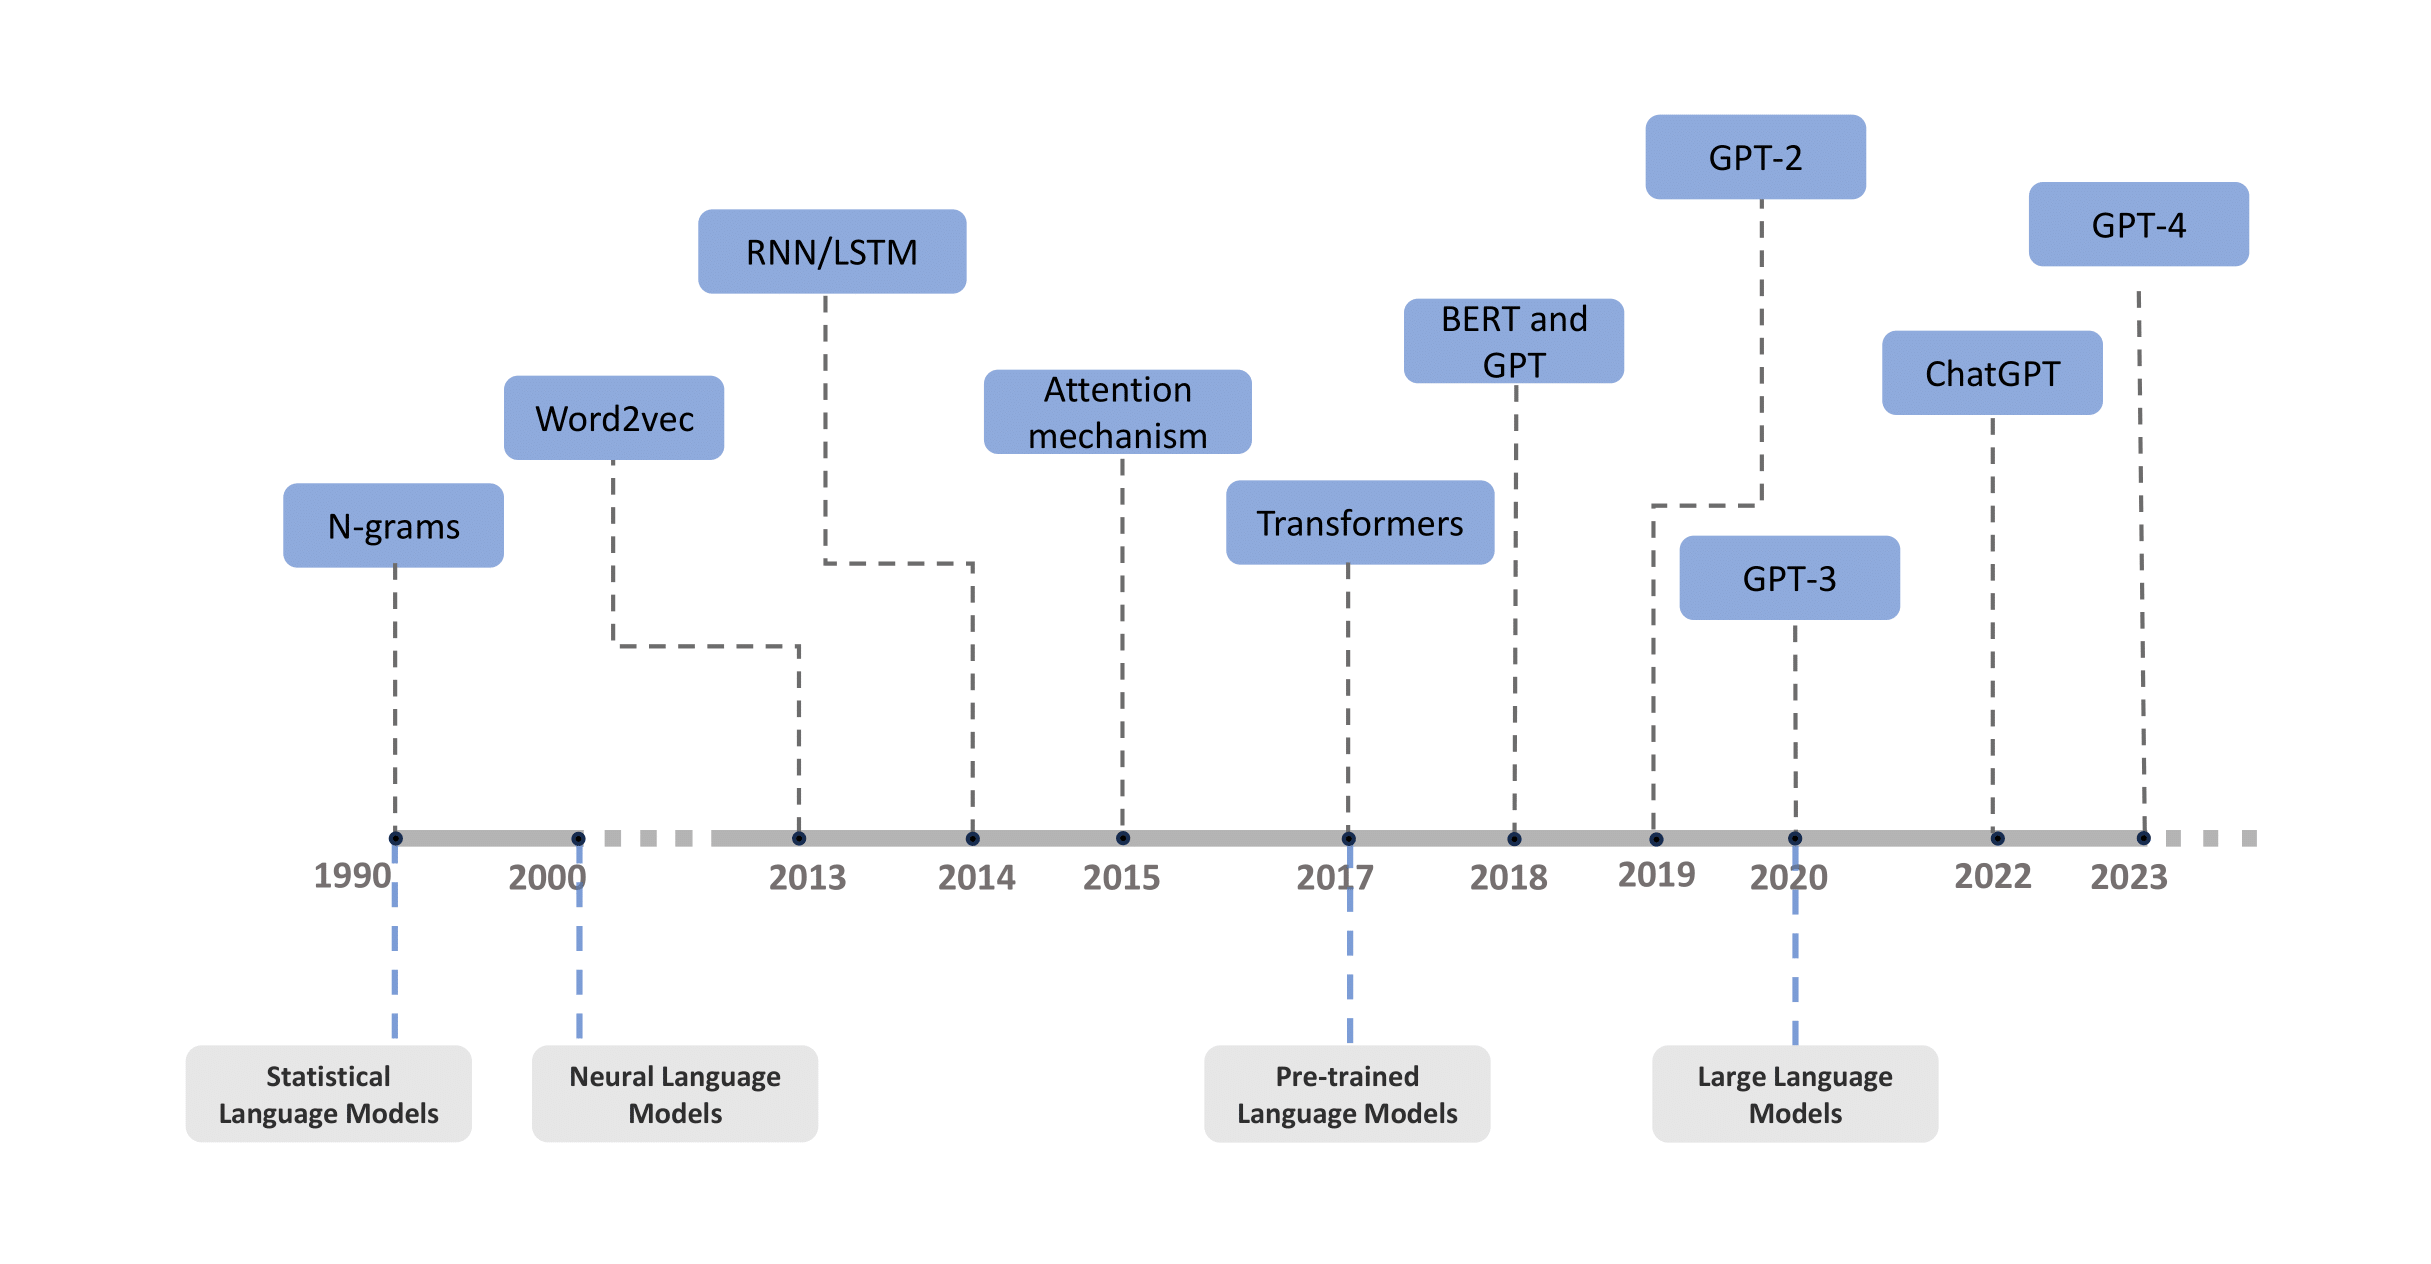
\includegraphics[width=1\linewidth]{img/Large Language Models and RAG/history.png}
    \caption[History and developmental stages of language models]{\textbf{History and developmental stages of language models}. Figure taken from~\cite{wang2024historydevelopmentprincipleslarge}. The historical progress in language processing models started with Statistical Language Models, which evolved into Neural Language Modeling. The next advancement was Pre-trained Language Models, with Large Language Models later on emerging as cutting-edge artificial intelligence systems~\cite{naveed2024comprehensiveoverviewlargelanguage}.}
    \label{fig:history}
\end{figure}

\paragraph{Statistical Language Models}\mbox{}\\

\noindent Originally developed in the 1990s, \emph{Statistical Language Models} (SLMs) emerged as mathematical models that use probabilistic methods to capture contextually relevant aspects in natural language. The principal idea behind them lies in estimating the likelihood of a sentence based on patterns from a large training corpus~\cite{wang2024historydevelopmentprincipleslarge, lau1994adaptive}. This estimation is typically done through \emph{Maximum Likelihood Estimation}:

\begin{equation} \label{eq:MLE}
    P(w_{i}|w_{1}w_{2}\cdots w_{i-1})=\frac{P(w_{1}\cdots w_{i-1}w_{i})}{P(w_{1} w_{2}\cdots w_{i-1})}=\frac{\mathbf{C}(w_{1}w_{2}\cdots w_{i})}{\mathbf{C}(w_{1}w_{2}\cdots w_{i-1})}
\end{equation}

Here, the numerator and denominator $\mathbf{C(\cdot)}$ represent the count of occurrences of the subsequences in the training set. This ratio estimates the probability by replacing the actual probabilities with observed frequencies in the training corpus. Essentially, the conditional probability of $i$-th word $\omega_i$ can be calculated given all the preceding words $\omega_1$ to $\omega_{i-1}$. Then, the $i$-th word is selected by choosing the word associated with the highest probability. This approach assumes that the $n$-th word is related to the initial $n$ - 1 words, which is commonly referred to as the n-gram model. 

However, the number of predictions grows exponentially with the size of the vocabulary, leading to storage problems and constraints~\cite{wang2024historydevelopmentprincipleslarge}. As a result, $n$ is typically limited to 2 or 3, which means the model only considers the last 1 or 2 words when predicting the next word, and the SLM's accuracy is reduced~\cite{wang2024historydevelopmentprincipleslarge}.

\paragraph{Neural Language Models}\mbox{}\\

\noindent Considering the limitations of the n-gram model, the next significant advancement in language modeling was introduced with the proposal of the \emph{Neural Language Model} (NLM)~\cite{10.1145/3490443,review10433480}. This model, proposed by Bengio et al.~\cite{bengio2003neural}, employs artificial neural networks and deep learning approaches to learn linguistic patterns and comprehend, generate, and predict human language~\cite{review10433480,wang2024historydevelopmentprincipleslarge}. Here, words or combinations of them are represented through real-valued vectors called word embeddings. Humans can effortlessly understand word meanings, but for computers to do the same, human language needs to be numerically translated. This is accomplished via word vectors, where each word corresponds to a unique vector.

Word embedding as a technique offers great efficiency and scalability, while the incorporation of a neural network significantly reduces the model's overall parameter count~\cite{10.1145/3490443}. In an NLM, the conditional probability is determined as follows~\cite{10.1145/3490443}:

\begin{equation}
    P(w_i \mid w_{i-n+1}, w_{i-n+2}, \ldots, w_{i-1}) = f_{\theta}(\mathbf{w}_{i-n+1}, \mathbf{w}_{i-n+2}, \ldots, \mathbf{w}_{i-1})
\end{equation}
where $(\mathbf{w}_{i-n+1}, \ldots, \mathbf{w}_{i-1})$ denote the embeddings of the words $\omega_{i-n+1}$, $\omega_{i-n+2}$,..., $\omega_{i-1}$. $f(\cdot)$ indicates the neural network and $\theta$ denotes the network parameters. At each position in the sequence, an intermediate representation is computed based on the word embeddings from the preceding $n-1$ positions. This process is applied consistently across all positions in the sequence. The resulting intermediate representation is then used to predict the word for the current position.

This approach laid the foundation for the development of a large number of word-embedding and modeling methods that rely on neural networks. Among representative methods for word embedding, we can mention Word2Vec~\cite{mikolov2013efficientestimationwordrepresentations}. As for neural language modeling, \emph{Recurrent Neural Networks}, including \emph{Long Short-Term Memory}~\cite{10.1162/neco.1997.9.8.1735} language models have been widely adopted due to their ability to capture temporal dependencies in sequences and model contextual relationships over time.

\paragraph{Pre-trained Language Models}\mbox{}\\

\noindent While conventional LMs are trained for specific tasks using supervised learning, \emph{Pre-trained Language Models} (PLMs) are trained in a self-supervised setting on large text corpora~\cite{10.1145/3649449}. The goal of this training is learning general-purpose representations that can be transferred across a wide range of tasks and surpass the performance of traditional LMs after fine-tuning for downstream tasks~\cite{naveed2024comprehensiveoverviewlargelanguage}. These models paved the way for the next era in \emph{natural language processing} (NLP) tasks~\cite{review10433480}. This initial training process is referred to as \emph{pre-training}. Once this stage is complete, the model can be adapted to a range of different NLP tasks, including translation, text generation, and question answering~\cite{review10433480}. To further enhance the performance on a specific task, the model undergoes a subsequent training phase on a smaller, task-specific dataset, a process called \emph{fine-tuning}. Together, these stages define the widely used \enquote{pre-training and fine-tuning} learning approach~\cite{wang2024historydevelopmentprincipleslarge}. 

The text generation objective for PLMs is defined as the following conditional probability of output text $y$ given the input data $x$~\cite{10.1145/3649449}:

\begin{equation}
    P(y \mid x) = \prod_{j=1}^{n}P(y_j \mid y_{<j}, x)
\end{equation}
where $y_j$ indicates the $j$-th output token and $y_{<j}$ indicates the preceding tokens $y_1$,..,$y_{j-1}$ where each token is drawn from a vocabulary.

Another key characteristic of PLMs is that they employ different types of architectures, largely in credit to Transformers~\cite{vaswani2017attention}, neural network architectures which possess powerful language representation capabilities~\cite{10.1145/3490443}. We can list the following basic ones~\cite{10.1145/3649449}:

\begin{enumerate}
    \item \emph{Encoder-Only} - Transformer-based language models using an encoder architecture leverage full attention mechanisms and are typically pre-trained using the masked language modeling objective, where the goal is to predict masked tokens by utilizing bidirectional context.
    
    \item \emph{Decoder-Only} - Decoder-only language models are tailored for tasks where the objective is to predict the next word based on all preceding ones. These models typically come in two forms: causal decoders and prefix decoders. Causal decoders utilize a strictly lower-triangular attention matrix (with zeros along the diagonal and lower part, and negative infinity in the upper part), restricting each token's attention to only earlier tokens. On the other hand, prefix decoders employ a hybrid attention mechanism, where the input section uses bidirectional attention, while the output section uses a lower-triangular matrix. This configuration allows input tokens to reference each other, while output tokens can attend to both all input tokens and the preceding output tokens.

    \item \emph{Encoder-Decoder} - Encoder-decoder language models adopt the classic Transformer framework for text generation, consisting of multiple layers of both encoders and decoders.
\end{enumerate}

Downstream NLP tasks can achieve significantly improved performance, even when only a small amount of annotated data is available~\cite{WANG202351}. The emergence of PLMs has enabled significant breakthroughs in NLP topics such as \emph{natural language understanding}, including sentiment analysis, document classification, reading comprehension, semantic matching, and information extraction~\cite{WANG202351}. It has also helped make advancements in \emph{natural language generation}, such as question generation, text summarization, and data-to-text generation~\cite{WANG202351}. The latter one has even undergone further advancements with pre-training on human-like conversations through social media data and enabled \emph{dialogue} generation~\cite{WANG202351}.

\section{Background of Large Language Models}

Increasing the size of PLMs has resulted in greater performance improvements, prompting a shift towards transitioning to LLMs, characterized by a significant increase in model parameters (tens to hundreds of billions)~\cite{review10433480} and size of training datasets (several gigabytes to terabytes)~\cite{naveed2024comprehensiveoverviewlargelanguage}. This advancement was backed up by LLMs' data diversity, computational advancement, and algorithmic innovation~\cite{wang2024historydevelopmentprincipleslarge}. Their key feature is combining large-scale pre-training with alignment to human values. In comparison to PLMs, LLMs are more adaptable, evolving from specialized to general-purpose models~\cite{wang2024historydevelopmentprincipleslarge}.

Figure~\ref{fig:llm_background} provides a general overview of the essential aspects associated with LLMs, which are detailed below.

\begin{figure}[H]
    \centering
    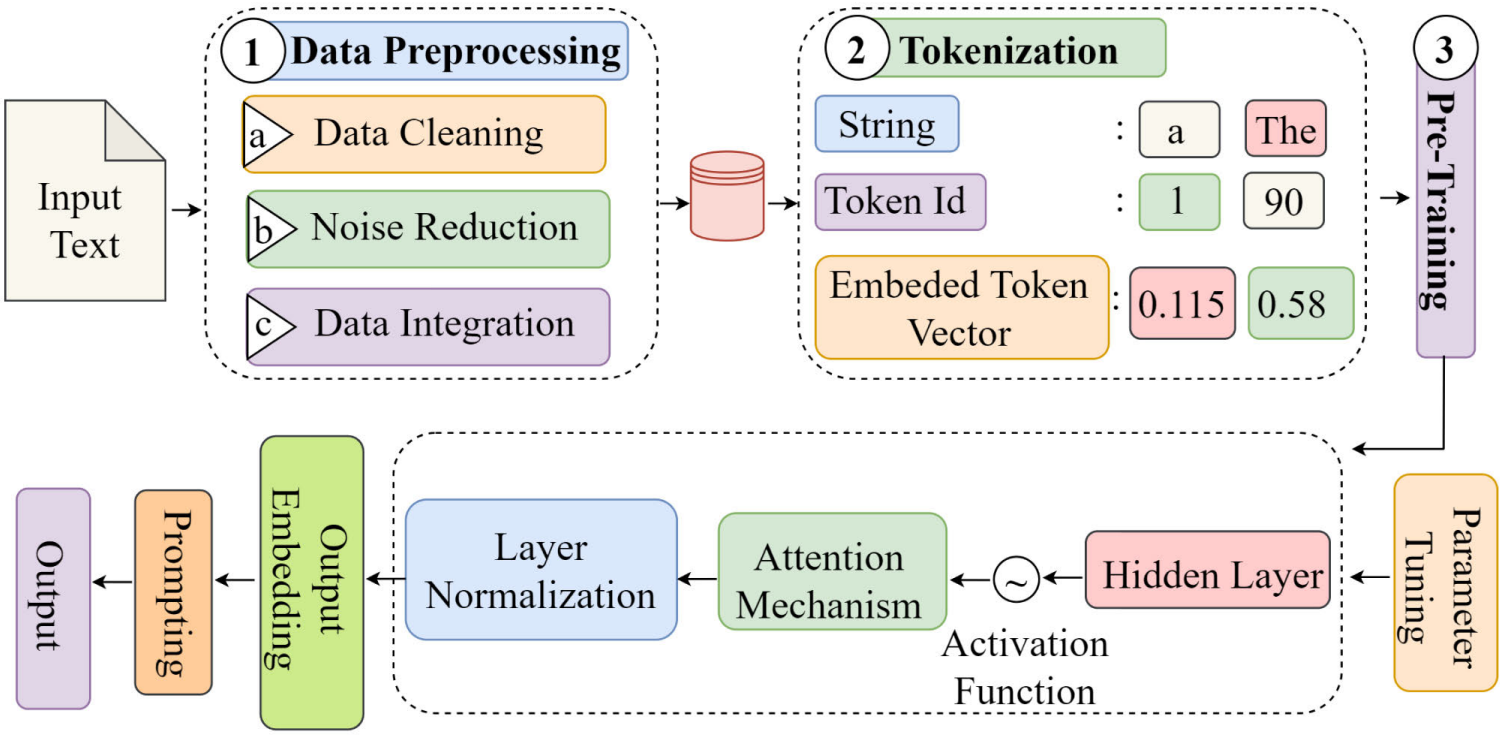
\includegraphics[width=0.9\linewidth]{img/Large Language Models and RAG/llm_background.png}
    \caption[Background of LLMs]{\textbf{Background of LLMs}. Figure taken from~\cite{review10433480}. Overview of core components and preparatory steps in LLM training and usage, including data preprocessing, tokenization, training frameworks, parameter tuning, neural architecture (activation functions, attention, and normalization), and prompting to receive an output.}
    \label{fig:llm_background}
\end{figure}
\noindent\emph{Data Preprocessing} - Data preprocessing for LLM training involves key techniques such as quality filtering, data deduplication, and privacy reduction~\cite{review10433480,naveed2024comprehensiveoverviewlargelanguage}. Quality filtering is responsible for removing low-quality or irrelevant data, while data deduplication prevents overfitting by eliminating repeated samples~\cite{review10433480}. Finally, privacy reduction methods help identify and filter out sensitive information like names and contact details, ensuring compliance and data security~\cite{review10433480,naveed2024comprehensiveoverviewlargelanguage}.

\noindent\emph{Tokenization} - This is an essential pre-processing step in NLP tasks~\cite{schmidt2024tokenizationcompression} that resolves around parsing text into discrete tokens~\cite{singh2024tokenizationcountsimpacttokenization}. These non-decomposing units~\cite{naveed2024comprehensiveoverviewlargelanguage} can be characters, symbols, subwords, or words depending on the model's characteristics and tokenization process~\cite{review10433480,naveed2024comprehensiveoverviewlargelanguage,10.1145/3624724}.

\noindent\emph{Training Frameworks} - LLM training approaches enlist several different methodologies such as Data Parallelism, Pipeline Parallelism, Model Parallelism, Tensor Parallelism, 3D Parallelism, and Optimizer Parallelism~\cite{review10433480,naveed2024comprehensiveoverviewlargelanguage}. For more details on these frameworks, see~\cite{naveed2024comprehensiveoverviewlargelanguage}.

\noindent\emph{Parameter Tuning} - Further model adaptations allow them to incorporate up-to-date information and enhance comprehension of user behavior~\cite{10.1145/3626772.3657807} within particular domains~\cite{bdcc9040087}. They also enable customization for specific applications~\cite{review10433480,bdcc9040087}.

\noindent\emph{Activation Function} - In neural architecture, activation functions determine if a neuron (node) should be activated or not~\cite{ignijic2024evaluating}. They play a crucial role in the curve-fitting capabilities of neural networks~\cite{activationfunction}.

\noindent\emph{Attention Mechanism} - This mechanism is utilized as a \enquote{resource allocation scheme} and is an increasingly common component of neural architecture~\cite{NIU202148}. It helps capture input sequence representations by forming links between different tokens~\cite{review10433480,11027973} and supports the models in processing complex contexts and domain-specific knowledge~\cite{guan2025attentionmechanismsperspectiveexploring}.

\noindent\emph{Layer Normalization} - Layer normalization is an integrated component of transformers. It is crucial for faster convergence and highlights their impact on stability during the training phases~\cite{review10433480,naveed2024comprehensiveoverviewlargelanguage}.

\noindent\emph{Prompting} - Prompts are text-based inputs that are provided to LLMs, processed, and used as guidance or alignments for output generation. LLMs are referred to as \emph{zero-shot} learners, which means that they are capable of responding to queries they have never seen before~\cite{naveed2024comprehensiveoverviewlargelanguage,bhandari2024surveypromptingtechniquesllms}.
Various prompting techniques and setups are currently being utilized, in regard to which the models' answers vary significantly. For example, \emph{few-shot prompting} provides a small number of examples for in-context learning while \emph{chain-of-thought prompting} decomposes complex tasks into logical steps~\cite{bhandari2024surveypromptingtechniquesllms}. Even more basic and advanced prompt engineering techniques exist, as it is an increasingly important topic for LLM output generation.

\section{Retrieval Augmented Generation}

\begin{figure}[htb!]
	\centering
	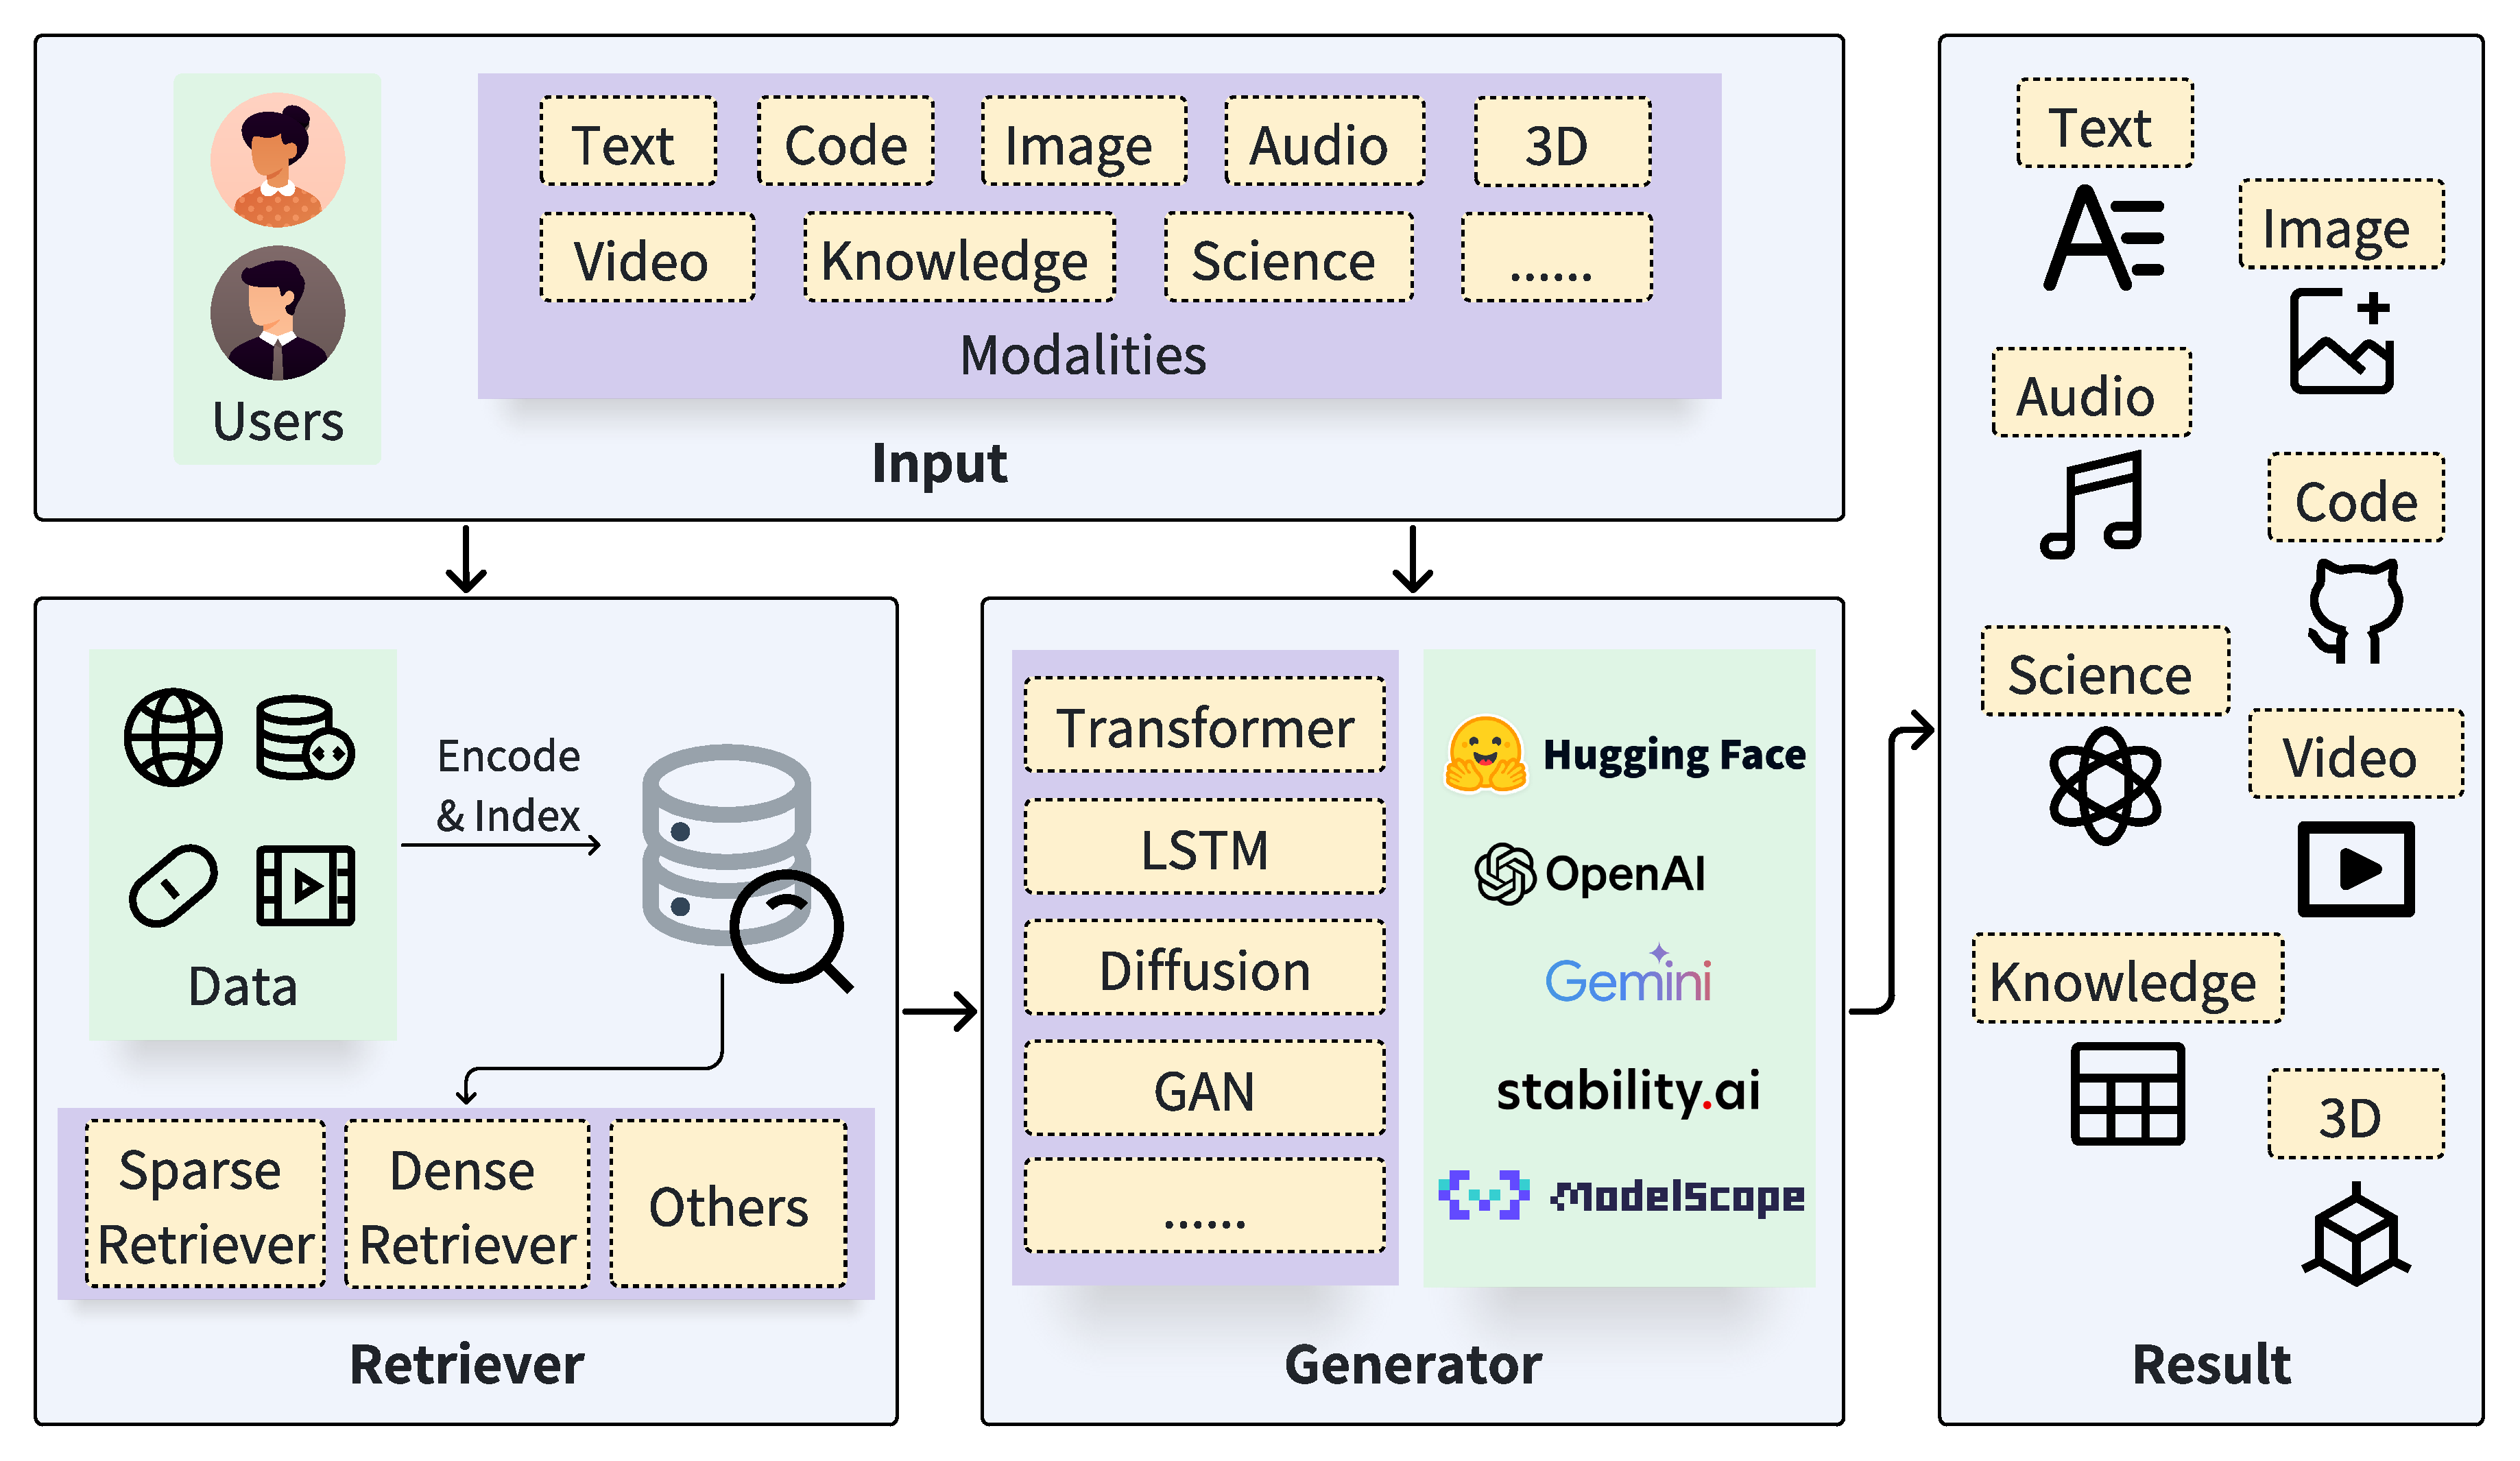
\includegraphics[width=1.0\linewidth]{img/Large Language Models and RAG/RAG_overview.pdf}
        \caption[A generic RAG architecture]{\textbf{A generic RAG architecture}. Figure taken from~\cite{zhao2024retrievalaugmentedgenerationaigeneratedcontent}. User queries are processed by both the retriever and the generator, where the retriever gathers relevant information from the provided data sources, and the generator uses it to produce responses across different modalities.}
	\label{fig:rag_overview}
\end{figure}

In several practical domains, LLMs are highlighted for their progressive enhancements throughout the years, contributing to the widespread popularity and implementation they have gained~\cite{rane2023contribution}. However, despite their impressive performances, these models still struggle with several challenges. Among them, we can mention issues with limited memory, outdated information~\cite{naveed2024comprehensiveoverviewlargelanguage}, lack of domain-specific knowledge, aka hallucination, and low accuracy of complicated tasks~\cite{gao2024retrievalaugmentedgenerationlargelanguage,liu2024raghelpreasoningllm,bartczak2024rag,wang2024evaluatingqualityanswersretrievalaugmented,10.14778/3685800.3685905,wang2024bioragragllmframeworkbiological}. To mitigate these limitations, the incorporation of RAG has shown a significant impact in improving and enhancing the capabilities of these models by integrating parameterized knowledge from external knowledge bases~\cite{naveed2024comprehensiveoverviewlargelanguage,gao2024retrievalaugmentedgenerationlargelanguage}. In essence, when generating responses, the model first retrieves relevant information from a large document corpus and utilizes it to enhance the prediction quality~\cite{gao2024retrievalaugmentedgenerationlargelanguage}. This approach reduces the need to retrain large models for tasks belonging to specific domains, making it a remarkable method for NLP tasks and other knowledge-intensive applications~\cite{10.1145/3626772.3657957}.

As shown in Figure~\ref{fig:rag_overview}, there are two major components in a RAG framework: a \emph{retriever} and a \emph{generator}~\cite{naveed2024comprehensiveoverviewlargelanguage,Yu_2025,zhao2024retrievalaugmentedgenerationaigeneratedcontent}. Initially, the retriever receives the input query from the user and proceeds to search for relevant information from the data located in the knowledge base~\cite{zhao2024retrievalaugmentedgenerationaigeneratedcontent}. In the RAG pipeline, the retriever's main role is to process and retrieve the top-k relevant
documents from the external corpus~\cite{gao2024retrievalaugmentedgenerationlargelanguage}. This process involves two stages, indexing and searching. Indexing structures and organizes provided documents to enable efficient retrieval, using inverted indexes for sparse retrieval or dense vector representations for dense retrieval~\cite{Yu_2025}. The searching module then leverages these indexes to identify documents relevant to a user's query, optionally using rerankers to refine or adjust the ranking of the retrieved documents~\cite{Yu_2025}. In the following step, the generator is fed the original query and the retrieved content through specific augmentation methodologies~\cite{zhao2024retrievalaugmentedgenerationaigeneratedcontent}. It then uses them to enhance the generation process and produce meaningful and contextually aware outputs by leveraging the prompting and inference phases~\cite{Yu_2025}.

In early RAG-implemented applications, the focus fell on the utilization of unstructured data, especially for open-domain question answering. Over time, the scope of retrievable knowledge sources broadened to include high-quality data, and this expansion currently encompasses even structured knowledge such as knowledge graphs~\cite{gao2024retrievalaugmentedgenerationlargelanguage}. For more details on the performance of this architecture, refer to section~\ref{rag_weaknesses}.

\chapter{Related Work} \label{chap:related_work}

Recent advancements in LLMs have sparked growing interest and contributed to the enablement of a range of applications focused on data analysis tasks, particularly in supporting non-expert users through natural language interfaces. We review existing systems and research to explore how LLMs, often in combination with external knowledge sources, are leveraged to automate or enhance analytical workflows. We then turn to evaluations of LLM performance on structured data tasks, followed by a discussion of the limitations in code-based data analysis and the integration of external knowledge through RAG. Together, these sections provide essential context for understanding both the potential and the current restrictions of the approach investigated in this work.

\section{LLM-driven Data Analysis Systems}

We now turn to existing LLM-empowered data analysis frameworks that closely align with the approach this paper is investigating the feasibility of. Their methodologies, along with the strengths and limitations of each strategy, are analyzed. These papers not only offer meaningful support for data analysts and decision-makers but also show strong potential for driving innovation and contributing to the further advancement of intelligent data analysis services.

\subsection{InsightPilot}

InsightPilot~\cite{ma2023demonstrationinsightpilotllmempoweredautomated} is an LLM empowered system designed to ease the time-consuming and demanding process of \emph{Exploratory Data Analysis} (EDA). Since EDA requires in-depth knowledge of the dataset and expertise in data analysis techniques, the authors propose leveraging LLMs to automate and drive this process.

InsightPilot places heavy emphasis on identifying trends and patterns from data, categorizing them into \emph{basic insights} (directly captured patterns) and \emph{compound insights} (built upon one or more existing insights). This system employs a pipeline of three main components. The first component is a user interface that allows natural language queries and displays the resulting analyses as both text and visualizations. The second one is an LLM that guides the exploration by selecting relevant insights and analytical goals based on contextual factors. The final one is an insight engine that performs the analysis and delivers the findings in natural language. It incorporates two OpenAI models, gpt-3.5-turbo~\cite{openai_gpt35_turbo} as the language model and textembedding-ada-002~\cite{openai_embedding_ada} to generate embeddings.

During this pipeline, the LLM performs four main analysis actions. Firstly, it \emph{identifies} high-level patterns using trend detection and translates trends into natural language. Secondly, it tries to \emph{summarize} by viewing the derived insight from multiple perspectives. Then, the model \emph{compares} the input insights from different neighbors (i.e., trends) and aims to identify compound insights. Finally, the model \emph{explains} the insight and highlights anomalies or differences in the data. This step reveals a limitation of the LLM, as the model generates hundreds of insights, with the majority of them being non-trivial or redundant. These redundant insights are filtered out by checking for entailment by more informative insights. The most relevant insights (top-$K$) are then selected using semantic similarity (via embeddings) and re-ranked for diversity.

As for the evaluation results, in a user study comprised of four independent data-science participants, InsightPilot outperformed existing solutions such as OpenAI Code Interpreter~\cite{openai_code_interpreter_tool} and Langchain Pandas Agent~\cite{langchain_pandas} in terms of relevance, completeness, and understandability.

\subsection{JarviX}

Similarly, JarviX~\cite{liu2023jarvixllmcodeplatform} is a system designed to facilitate automated guides and perform high-precision analyses and visualizations on tabular data. It was specifically created to allow and equip non-experts to conduct advanced analytics through a rule-based framework. The base LLM that is employed in this experimentation is vicuna-13b1.1-gptq-4bit-128g~\cite{vicuna-13B-1.1-GPTQ-4bit-128g}.

Once structured or unstructured data is uploaded, JarviX automatically cleans and preprocesses it while detecting data types and computing statistics. Without disrupting user flow, correlation matrices are generated. It then collects metadata and employs the model to produce a data summary report, highlighting key characteristics and suggesting the ten most relevant analytical questions. A rule-based \emph{Question Matcher} maps user queries to backend modules using SQL matching by detecting keywords such as those related to columns, constraints (e.g., “top 10”), and analysis methods. For users with specific goals, JarviX also offers visualizations and insights, adds domain knowledge, and suggests follow-up analyses or complete reports. To ensure response quality, prompt engineering is used, where initial manually structured prompts are refined through feedback loops using GPT-4~\cite{openai2024gpt4technicalreport} until performance benchmarks are met. This enables JarviX to reliably support tasks like anomaly detection, root cause analysis, and forecasting.

JarviX is evaluated across a variety of open-source tabular datasets to assess its performance in natural language question matching. The performance results, summarized in Table~\ref{tab:jarvix_question_matching}, focus on column name recognition, user intent detection, and constraint handling. JarviX performs well in identifying individual columns and responds more accurately to queries with clear intent. However, it occasionally struggles with multi-column questions and ambiguous phrasing, leading to over- or under-identification of relevant terms.

\begin{table}[h]
\centering
\begin{tabularx}{\textwidth}{l *{3}{>{\centering\arraybackslash}X >{\centering\arraybackslash}X}}
\toprule
\multirow{2}{*}{\textbf{Data Source}} 
& \multicolumn{2}{c}{\textbf{Column Name}} 
& \multicolumn{2}{c}{\textbf{Intention}} 
& \multicolumn{2}{c}{\textbf{Restriction}} \\
\cmidrule(lr){2-3} \cmidrule(lr){4-5} \cmidrule(lr){6-7}
& \textbf{Top 1} & \textbf{Top 3} 
& \textbf{Top 1} & \textbf{Top 3} 
& \textbf{Top 1} & \textbf{Top 3} \\
\midrule
Manufacture    & 72.0 & 83.3 & 74.0 & 82.7 & 64.7 & 72.0 \\
Sport          & 73.3 & 88.3 & 75.0 & 90.8 & 65.8 & 76.7 \\
Sales          & 70.7 & 82.7 & 77.3 & 86.7 & 67.3 & 78.7 \\
Food           & 69.2 & 88.3 & 75.8 & 90.8 & 70.0 & 77.5 \\
Health Care    & 65.0 & 74.2 & 73.3 & 85.0 & 67.5 & 74.2 \\
Banking        & 81.7 & 93.3 & 79.2 & 91.2 & 66.7 & 74.2 \\
\bottomrule
\end{tabularx}
\caption[Evaluation results for question matching]{\textbf{Evaluation results for question matching}. Table taken from~\cite{liu2023jarvixllmcodeplatform}. \enquote{Top 1} refers to the instances where the correct result was identified as the top most result, while \enquote{Top 3} refers to the instances where the correct result was found within the top three results.}
\label{tab:jarvix_question_matching}
\end{table}

\subsection{Chat2Data}

In an effort to provide a framework that eliminates the knowledge-based barriers to entry on data analysis methods for ordinary users who cannot write programming scripts and SQL queries, Zhao, Zhou, and Li introduce Chat2Data~\cite{10.14778/3685800.3685905}. Chat2Data is an interactive data analysis system that uses LLMs and RAG to make data analysis easier and more beginner-friendly.

Chat2Data facilitates natural language and multi-turn dialogues with users to simplify data interaction, aiming for low-code or sometimes even zero-code usability. It processes domain data by segmenting it semantically into paragraphs, generating embeddings for each one, and storing them in a vector database. This system enables users to upload various file types, including JSON, Excel, and PDF, for processing and indexing in the vector database. When a user submits a natural language query, Chat2Data retrieves relevant context by comparing the query's embedding with those in the database and uses the results to prompt the LLM. For unstructured data, it leverages LLMs to produce summaries, while for structured data, it translates queries into SQL and uses pandas APIs for data visualization. To optimize performance, this framework also caches frequent queries in the vector database and returns cached results directly when possible, thus bypassing LLM interaction at times.

To enable some of these capabilities, Chat2Data incorporates RAG for augmenting domain knowledge. It uses a fine-tuned Llama2~\cite{touvron2023llama2openfoundation} model for translating natural language queries to pandas APIs and processing of complicated tasks. In this paper, the performance of Chat2Data is assessed on Apple product knowledge and Kaggle datasets on Netflix Movies and TV Shows, showcasing the prototype's ability to handle data analysis on unstructured and structured data.

\subsection{BIORAG}

BIORAG~\cite{wang2024bioragragllmframeworkbiological} is a framework that combines LLMs with RAG to address the complexity of biological knowledge systems and improve biological question reasoning. To keep up with emerging biology information, BIORAG adaptively selects knowledge from external data sources.

High-quality domain-specific corpora are essential for improving embedding models in biological question-answering systems. To achieve this, BIORAG extracts and filters research papers from the NCBI\footnote{\url{https://www.ncbi.nlm.nih.gov/}}'s global biomedical article database and integrates various biological insight databases. To stay up to date with the latest developments and peer-reviewed literature, BIORAG leverages multiple search engines, including Google, Bing, arXiv, Wikimedia, and Crossref.

BIORAG introduces a self-evaluated retrieval mechanism that combines keyword-based filtering with vector-based semantic search to improve retrieval accuracy and contextual understanding. It utilizes a fine-tuned embedding model built on PubMedBERT~\cite{10.1145/3458754}, which is optimized using contrastive learning techniques to rank and retrieve relevant biomedical content. A multi-step reasoning process guides the system. It preprocesses queries, retrieves information, evaluates its relevance, and iterates if needed. This enables BIORAG to handle ambiguous or complex queries by dynamically switching between local databases and external sources.

In an experiment where Llama3-70B~\cite{metallama3} is used as the main model, this system is evaluated on six biology-related QA benchmarks, with comparisons against a range of baselines including general-purpose LLMs, \emph{biology-focused LLMs} (BioLLMs), and \emph{scientific RAG-LLM frameworks} (SciRAG). As shown in Table~\ref{tab:biorag_res}, BIORAG outperforms all baselines across all biological QA datasets, despite some of the baselines' large size and external tool integrations. This strong performance in handling complex biological queries is attributed to the integration of both internal and external sources. An ablation study by the authors reveals that specific integrated databases are crucial to the framework's accuracy. Furthermore, larger models like Llama3-70B consistently outperform their smaller counterparts.

\begin{table}[h]
\centering
\resizebox{\linewidth}{!}{
\begin{tabular}{lcccccccccccc}
\toprule
\multirow{2}{*}{} & \multicolumn{3}{c}{\textbf{LLM}} & \multicolumn{2}{c}{\textbf{BioLLM}} & \multicolumn{2}{c}{\textbf{SciRAG}} & \multirow{2}{*}{\textbf{BioRAG} } \\
\cmidrule(lr){2-4} \cmidrule(lr){5-6}  \cmidrule(lr){7-8}  
& GPT3.5 & Llama3-8B &  Llama-70B & PMC-Llama & BioMistral & GeneGPT & NewBing  & \\
\midrule
MedMCQA & 54 & 51 &  \underline{71} & 56 & 49 & 0 & 55 & \textbf{73} \\
Medical Genetics &  \underline{74} & 51 & 67 & 28 & 67 & 0 & \textbf{88} & \textbf{88} \\
College Biology & 73 & 75 &  \underline{88} & 30 & 67 & 0 & 71 & \textbf{90} \\
College Medicine & 65 & 61 & \underline{70} & 23 & 51 & 0  & \textbf{78}  & \textbf{78} \\
\bottomrule
\end{tabular}}
\caption[Performance of BioRAG compared to other RAG-LLMs on the biological-related QA benchmarks]{\textbf{Performance of BioRAG compared to other RAG-LLMs on the biological-related QA benchmarks}. Table taken from~\cite{wang2024bioragragllmframeworkbiological}. The scores represent accuracy. \textbf{Bold} and \underline{underlined} results denote the highest and second-highest performance, respectively.}
\label{tab:biorag_res}
\end{table}

\subsection{Financial Analysis}

In a research focused on developing an intelligent financial data analysis system~\cite{wang2025financialanalysisintelligentfinancial}, the authors suggest that implementing RAG overcomes the insufficient domain-specific knowledge and challenges of basic LLMs. By incorporating a comprehensive dataset of NASDAQ\footnote{\url{https://www.nasdaq.com/}} financial fundamentals into the system's external knowledge base, the framework aims to deliver more accurate and insightful financial analyses.

\begin{table}[ht]
\centering
\begin{tabular}{lcc}
\toprule
\textbf{Model} & \textbf{Accuracy Rate} & \textbf{Recall} \\
\midrule
gpt-3.5-turbo              & 55.6\% & 78.3\% \\
gpt-3.5-turbo+RAG          & 63.7\% & 88.7\% \\
gpt-3.5-turbo-1106         & 59.3\% & 85.4\% \\
gpt-3.5-turbo-1106+RAG     & 78.6\% & 89.2\% \\
\bottomrule
\end{tabular}
\caption[GPT models' performance on financial tasks]{\textbf{GPT models' performance on financial tasks}. Table adapted from~\cite{wang2025financialanalysisintelligentfinancial}. The accuracy and recall of various GPT models with and without RAG incorporation, evaluated on financial data analysis tasks.}
\label{tab:financial_analysis_res}
\end{table}

In an evaluation of the system (see Table~\ref{tab:financial_analysis_res}), the results indicate that while baseline models demonstrate some moderate ability to perform financial data analysis tasks, the integration of RAG technology led to substantial performance improvements across all model variants. The basic models' performance can be attributed to a limited understanding of financial terms and knowledge gaps. The inclusion of RAG enables these models to efficiently access and incorporate that missing knowledge.


\section{Performance of LLMs Utilized in Advanced Data Analysis}

In the context of data analysis tasks, LLMs can address the limitations of existing machine learning algorithms, particularly in adapting to different databases, different hardware environments, and different query workloads~\cite{zhou2024llmenhanceddatamanagement,10.14778/3685800.3685838}. A task closely aligned with the goals of this research is providing users with the ability to navigate through databases while overcoming these limitations.  One of such methods, Text-to-SQL~\cite{rajkumar2022evaluatingtexttosqlcapabilitieslarge}, involves mapping natural language queries into SQL queries, allowing non-experts to explore and analyze database data, a task revolutionized by the emergence of LLMs~\cite{10.1145/3737873}. An empirical evaluation demonstrates that, without any fine-tuning, LLMs trained on code perform remarkably well with respect to their Text-to-SQL capabilities~\cite{rajkumar2022evaluatingtexttosqlcapabilitieslarge}. In many real-world data analysis scenarios, users who struggle with programming or writing SQL queries prefer using LLMs to enable natural language querying instead~\cite{zhou2024llmenhanceddatamanagement}. However, despite these models displaying enhanced performance in their overall generalization ability, adaptability, and potential for further improvements, they often lead to non-executable queries or results that do not align with user expectations~\cite{zhou2024llmenhanceddatamanagement}. Similarly, several challenges and concerns have been raised about their utility in this domain~\cite{10.1145/3737873}.

\subsection{Challenges in LLM-Based Data Analysis Systems}

A key challenge in leveraging LLMs for data analysis lies in the lack of a unified framework capable of handling diverse data types~\cite{zhou2025surveyllmtimesdata,zhou2024llmenhanceddatamanagement}. Currently, efficiently analyzing various data formats often requires the development of separate, task-specific, tuned models. While integrating several models into a single system seems like a straightforward solution, it significantly increases deployment and maintenance costs due to the complexity of managing multiple components~\cite{zhou2025surveyllmtimesdata}.

Another challenge is the effective utilization of proprietary knowledge~\cite{zhou2025surveyllmtimesdata,10.1145/3613905.3651042,10.1145/3737873}, where current methodologies rely heavily on fine-tuned models or RAG to bridge this gap. However, these approaches also struggle when dealing with recently updated or highly complex domain knowledge, often leading to generalization issues~\cite{zhou2025surveyllmtimesdata}. Their extensive training allows LLMs to grasp a broad array of concepts and terminology, but they often fall short in interpreting meanings that are specific to particular organizations or subtle contextual nuances~\cite{10.1145/3613905.3651042}. The lack of datasets that explicitly integrate such knowledge further worsens the problem, posing challenges for practical deployment in real-world industrial settings~\cite{zhou2025surveyllmtimesdata}. 

Although users value the support provided by LLMs, they also highlight the importance of transparency and the ability to validate outputs~\cite{10.1145/3613905.3651042}. Trust becomes a crucial concern, driven by the absence of ways to verify the tool's responses~\cite{10.1145/3613905.3651042}. Other significant challenges include privacy concerns and data governance~\cite{10.1145/3737873}, which remain difficult, particularly due to issues like ambiguity and semantic mismatch. Ambiguity occurs when multiple semantically different queries produce valid responses to the same natural language question, making it harder to assess the model's accuracy~\cite{10.1145/3737873}. Semantic mismatch arises when user queries express intents that cannot be fully or partially answered by the underlying database~\cite{10.1145/3737873}.

\begin{figure}[htb!]
	\centering
	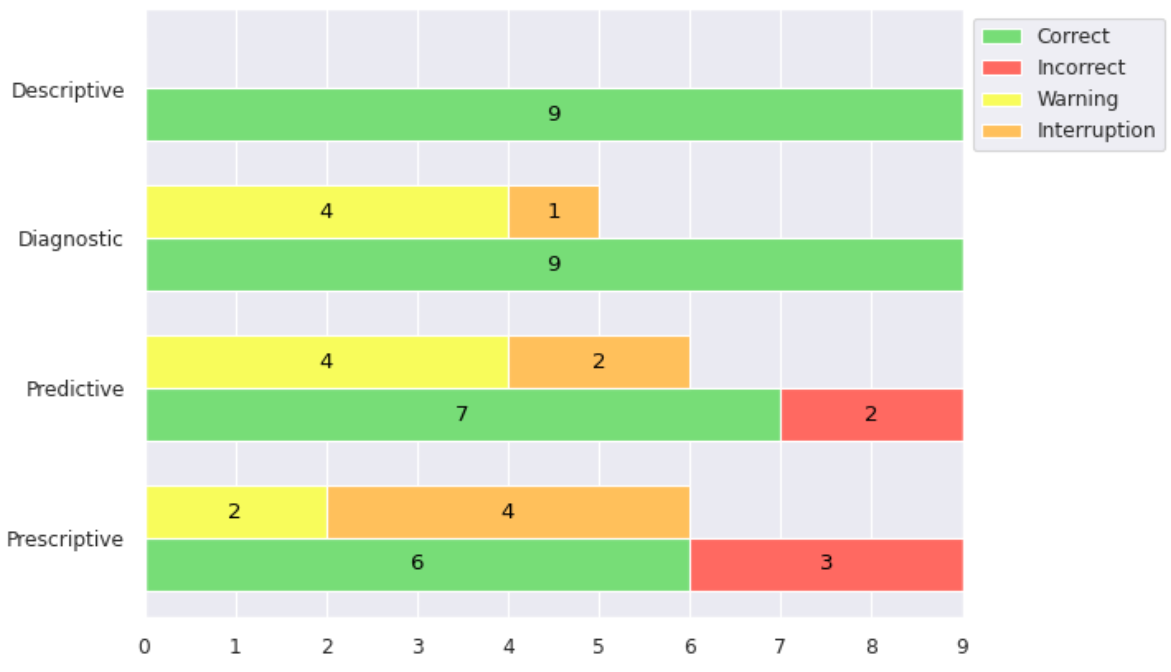
\includegraphics[width=0.75\linewidth]{img/Related Work/gpt_data_analyst_results.png}
	\caption[Summarization of the ChatGPT Data Analyst results]{\textbf{Summarization of the ChatGPT Data Analyst results}. Figure taken from~\cite{sbbd}. Summary of the obtained results, showing the number of responses and issues identified per category.}
	\label{fig:gpt_data_analyst_results}
\end{figure}

An evaluation of an LLM-based automated data analysis tool~\cite{sbbd} built around ChatGPT Data Analyst\footnote{\url{https://chatgpt.com/g/g-HMNcP6w7d-data-analyst}} shows strong performance in descriptive and diagnostic tasks but notable shortcomings in predictive and prescriptive analyses (see Figure~\ref{fig:gpt_data_analyst_results}). Across all categories, a considerable number of warnings and disruptions were observed. Despite generally solid results, the tool's 13.89\% error rate, 27.78\% warning rate, and 19.44\% interruption rate raise concerns regarding large models' reliability and operational robustness, especially in complex tasks requiring higher computational power. The system also displays tendencies toward operational breakdowns and the characteristic LLM hallucinations. These limitations, along with the lack of support for comprehensive data analysis libraries, negatively impact both the efficiency and consistency of the analytical process.

Another important consideration is the matter of choosing what type of model to employ for tasks of this scope. A survey indicates that the performance disparity between open-source and closed-source language models has considerably decreased, and that even smaller, fine-tuned open-source models now demonstrate promising potential to rival the capabilities of much larger LLMs~\cite{10.1145/3737873}. Both fine-tuned open-source models and closed-source models enhanced through prompt engineering have shown strong effectiveness in tackling core semantic parsing tasks~\cite{10.1145/3737873}.

\subsection{Limitations in Code-Based Data Analysis}

Using LLMs for code generation in data analysis automation systems has also proven to be not fully reliable. In qualitative research, while serving as valuable tools, LLMs can't completely replace human insights, especially in theory building or interpretation~\cite{chew2023llmassistedcontentanalysisusing}. In other tasks, a trade-off between code executability and accuracy can be observed. This becomes prominent as the complexity of the task increases, where in some cases the executability rate drops significantly and isn't necessarily improved by highly structured prompts~\cite{10.1371/journal.pone.0317084}. If a model's generated code fails to run, automatically returning it alongside the error for correction substantially improves code executability~\cite{10.1371/journal.pone.0317084}. However, executable code is not always reliable or correct~\cite{https://doi.org/10.1002/smr.2723}, highlighting the need for human validation, particularly for highly complex tasks~\cite{10.1371/journal.pone.0317084}.

Another study found that tasks such as conducting data analysis and visualizations across multiple sequential queries produce more diverse results~\cite{https://doi.org/10.1002/smr.2723}. For example, some tools fail to capture key details, resulting in inaccurate or misleading analyses, which pose a risk to the integrity of the findings. Identifying such inaccuracies can be difficult, particularly when the tool's capabilities surpass the user's expertise~\cite{https://doi.org/10.1002/smr.2723}. 

While LLMs show great promise in enhancing scientific productivity, current systems remain only partially reliable. They can support coding and analytical tasks, but their outputs must be carefully evaluated, especially in high-stakes scientific applications~\cite{https://doi.org/10.1002/smr.2723}.

\section{Pitfalls and Limitations of RAG} \label{rag_weaknesses}

Despite being primarily employed to reduce hallucinated responses in LLM-based tasks, RAG systems remain vulnerable to generating them as well~\cite{10921633}. While effective in incorporating external knowledge, RAG's performance can be compromised by imperfect retrieval and knowledge conflicts, which may introduce misleading, irrelevant, or potentially harmful content~\cite{wang2025astuteragovercomingimperfect,10921633}. Errors in the selection or ranking of relevant documents can degrade the quality of generated outputs~\cite{10.1145/3701716.3715490}, while knowledge conflicts can arise between the LLM's internal knowledge and the RAG's external knowledge~\cite{wang2025astuteragovercomingimperfect}. In a comprehensive analysis that focuses on questions from the diverse NQ~\cite{kwiatkowski2019natural}, TriviaQA~\cite{joshi2017triviaqa}, BioASQ~\cite{tsatsaronis2015overview}, and PopQA~\cite{mallen2023not} datasets, an estimated 70\% of the retrieved responses were revealed to not directly include correct answers (as shown in Figure~\ref{fig:RAG_retrieval_precision}). Additionally, it was observed that a lower retrieval precision leads to a higher knowledge conflict in general. This tight correlation highlights the need for mutual correction between the internal and external knowledge in order to mitigate and recover from RAG-related failures~\cite{wang2025astuteragovercomingimperfect}. Another common challenge is the inability to produce a response when only a limited number of document chunks are passed to the LLM~\cite{10921633}. This issue may be caused by various factors, such as an incomplete dataset, weak generative capabilities, a poor embedding model, or poorly formulated prompts~\cite{10921633}. Between a hallucinated response and a no-response scenario, the latter is preferred~\cite{10921633}.

\begin{figure}[h]
    \centering
    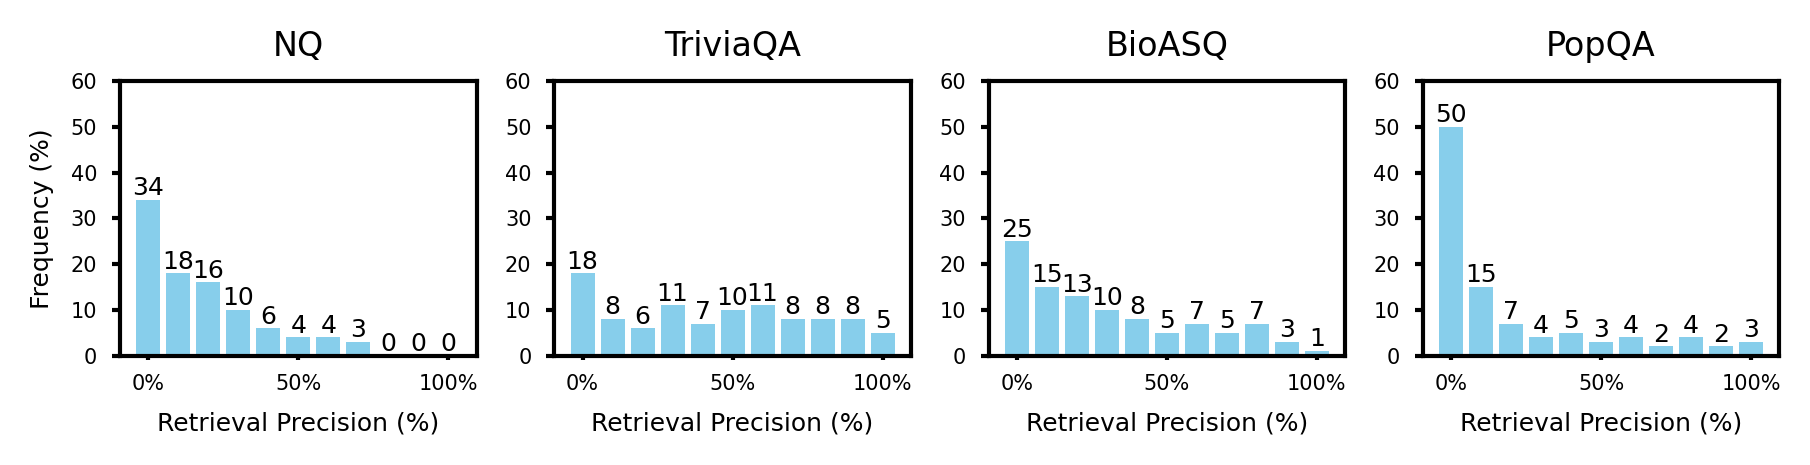
\includegraphics[width=1\linewidth]{img/Related Work/RAG_retrieval_precision.png}
    \caption[Imperfect retrieval in RAG]{\textbf{Imperfect retrieval in RAG}. Figure taken from~\cite{wang2025astuteragovercomingimperfect}. Distribution of retrieval precision across the four datasets. Each bar plot shows how often different precision levels occur.}
    \label{fig:RAG_retrieval_precision}
\end{figure}

RAG implementation also does not consistently lead to higher accuracy. Performance can vary across various models (see Table~\ref{tab:norag_rag_adapted}), with No RAG and RAG methods each outperforming the other in different cases. LLMs often struggle to extract correct information from external documents when the question-related information is distant from the answer-related one, an issue most common in longer texts~\cite{Chen_Lin_Han_Sun_2024}. This phenomenon is referred to as long-distance information~\cite{Chen_Lin_Han_Sun_2024}, a scenario in which, among several answer options, the model chooses the one where the question and answer-related information are closer. You can refer to Table~\ref{tab:rag_error_types_adapted} for an example. Another frequent issue is concept confusion, where the definitions or naming conventions in a document may be similar to the ones mentioned in the question~\cite{Chen_Lin_Han_Sun_2024}. In the example presented in Table~\ref{tab:rag_error_types_adapted}, the model wrongfully focuses on the term \enquote{automotive revenue} instead of just \enquote{revenue}. The aforementioned issues and noise are prevalent in complex questions asked to RAG-enhanced LLMs~\cite{Chen_Lin_Han_Sun_2024}.

\begin{table}[h]
    \centering
    \small
    \setlength{\tabcolsep}{4pt}
    \begin{tabular}{l@{\hskip 8pt}cccc|cccc}
        \toprule
         Method & \multicolumn{4}{c|}{\cellcolor{gray!15}\textit{Claude 3.5 Sonnet (20240620)}} & \multicolumn{4}{c}{\cellcolor{gray!15}\textit{Gemini 1.5 Pro (002)}} \\ \cmidrule(lr){2-5} \cmidrule(lr){6-9}
         & NQ & TriviaQA & BioASQ & PopQA & NQ & TriviaQA & BioASQ & PopQA \\ \midrule
        No RAG   & \textbf{47.1} & \textbf{82.0} & 50.4 & 29.8 & \textbf{44.8} & \textbf{80.2} & 45.8 & 25.3 \\ 
        RAG    & 44.4 & 76.7 & \textbf{58.0} & \textbf{36.0} & 42.7 & 76.0 & \textbf{55.2} & \textbf{33.7} \\ \midrule
         Method & \multicolumn{4}{c|}{\cellcolor{gray!15}\textit{Mistral-Large (2407), 128B}} & \multicolumn{4}{c}{\cellcolor{gray!15}\textit{Mistral-Nemo (2407), 12B}} \\ \cmidrule(lr){2-5} \cmidrule(lr){6-9}
         & NQ & TriviaQA & BioASQ & PopQA & NQ & TriviaQA & BioASQ & PopQA \\ \midrule
        No RAG & \textbf{46.8} & \textbf{79.5} & 43.7 & 24.7 & 29.8 & \textbf{67.8} & 34.3 & 23.0 \\ 
        RAG & 43.1 & 77.4 & \textbf{55.9} & \textbf{36.0} & \textbf{39.3} & 66.8 & \textbf{49.0} & \textbf{32.6} \\ 
        \bottomrule
    \end{tabular}
    \caption[Zero-shot accuracy results using No RAG and RAG methods across four models]{\textbf{Zero-shot accuracy results using No RAG and RAG methods across four models}. Table adopted from~\cite{wang2025astuteragovercomingimperfect}. The scores represent accuracy. \textbf{Bold} denote the highest performance between the two methods per model and dataset.}
    \label{tab:norag_rag_adapted}
\end{table}

Noise in the used datasets is one of the most frequent causes of inaccuracy in these systems~\cite{10921633}. Inevitable noise, such as misleading information or irrelevant content, can introduce critical failure points~\cite{zhao2024retrievalaugmentedgenerationaigeneratedcontent}. Given RAG's widespread adoption, the impact of noisy information in retrieved content has raised concerns, especially in risk-sensitive domains~\cite{wang2025astuteragovercomingimperfect}. Overall, ensuring that RAG-integrated external knowledge enhances outputs without compromising coherence or relevance remains a challenging and unresolved issue~\cite{10921633}.

\begin{table}[h]
    \centering
    \small
    \begin{tabular}{p{1.5cm}|p{6cm}|p{6cm}}
    \toprule
    \multicolumn{1}{c|}{} & \multicolumn{1}{c|}{\textbf{Long-distance information}} & \multicolumn{1}{c}{\textbf{Concept confusion}} \\
    \midrule
    \textbf{Question} & Who did Iga Swiatek defeat to win the Qatar Open 2022? & What was Tesla's revenue in Q1 2022? \\
    \midrule
    \textbf{Answer} & \textbf{Anett Kontaveit} & \textbf{18.76 billion} \\
    \midrule
    \textbf{Docs} & 
    \emph{Positive document}\newline
    Swiatek entered into the \textbf{Qatar Open} ...won ... \textbf{Anett Kontaveit} \newline
    \newline
    \emph{Negative document}\newline
    ... she defeated \emph{Ons Jabeur} 6-2, 7-6(5) to win the \emph{2022 US Open}
    & 
    \emph{Positive document}\newline \textbf{Tesla, Inc. reported Q1 FY 2022} ... revenues of \$\textbf{18.76 billion} \newline
    \newline
    \emph{Negative document}\newline
    ...\textbf{earnings for 2022} ... \emph{Automotive revenue }reached \$\emph{16.86 billion} \\
    \midrule
    \textbf{Response} & Iga Swiatek defeated \emph{Ons Jabeur} & ... in Q1 2022 was \$\emph{16.86 billion}. \\
    \bottomrule
    \end{tabular}
    \caption[Error cases of noise robustness]{\textbf{Error cases of noise robustness}. Table adapted from~\cite{Chen_Lin_Han_Sun_2024}. For each case, only one positive document and one negative document are shown. The \textbf{bold} text indicates the matching parts between the document and the question or answer, while the italicized text highlights the non-matching parts.}
    \label{tab:rag_error_types_adapted}
\end{table}

Another limitation is the need for real-time updated information, which introduces latency~\cite{10.1145/3701716.3715490,zhao2024retrievalaugmentedgenerationaigeneratedcontent,gao2024retrievalaugmentedgenerationlargelanguage}. Moreover, the combination of external retrieval and generation components increases system complexity~\cite{zhao2024retrievalaugmentedgenerationaigeneratedcontent} and computational cost~\cite{10921633,gao2024retrievalaugmentedgenerationlargelanguage}, requiring precise tuning and contributing to maintenance overhead~\cite{10.1145/3701716.3715490,zhao2024retrievalaugmentedgenerationaigeneratedcontent}. A major drawback of RAG is also the significant increase in context length, which can exceed the model's context window, an issue particularly evident for query-based RAG~\cite{zhao2024retrievalaugmentedgenerationaigeneratedcontent}. This extended context poses feasibility issues alongside slowing the overall generation process down~\cite{zhao2024retrievalaugmentedgenerationaigeneratedcontent}.

It is also important to note that currently there is no standardized evaluation methodology for RAG systems since it introduces several complexities~\cite{Yu_2025}, with various frameworks relying on different metrics for assessing them~\cite{10921633}. The difficulty in evaluating RAG systems is caused by both the retrieval and generation stages, each requiring thoughtful consideration and analysis~\cite{Yu_2025}. Chosen metrics must account for task-specific generative quality, user requirements, and practical system constraints~\cite{Yu_2025}. While currently established benchmarks tackle one or several of these aspects, developing a comprehensive assessment remains a challenging task~\cite{Yu_2025}.

Drawbacks in the implementation of RAG aren't limited to only internal cases. For instance, retrieval data leakage refers to an attack in which information from the provided dataset is exposed to an unauthorized individual~\cite{ammann2024analysis}. In some applications, the external documents include sensitive data such as personally identifiable information or any domain-specific knowledge that can be exploited~\cite{ammann2024analysis}. The greater the sensitivity of the data, the greater the risk of exposure. Caution is issued regarding attacks that are utilized in retrieving information from embedding and prompting processes, which are highly relevant in RAG implementations focused on sensitive data~\cite{ammann2024analysis}.

\chapter{Methodology} \label{chap:methodology}

\begin{figure}[!b]
    \centering
    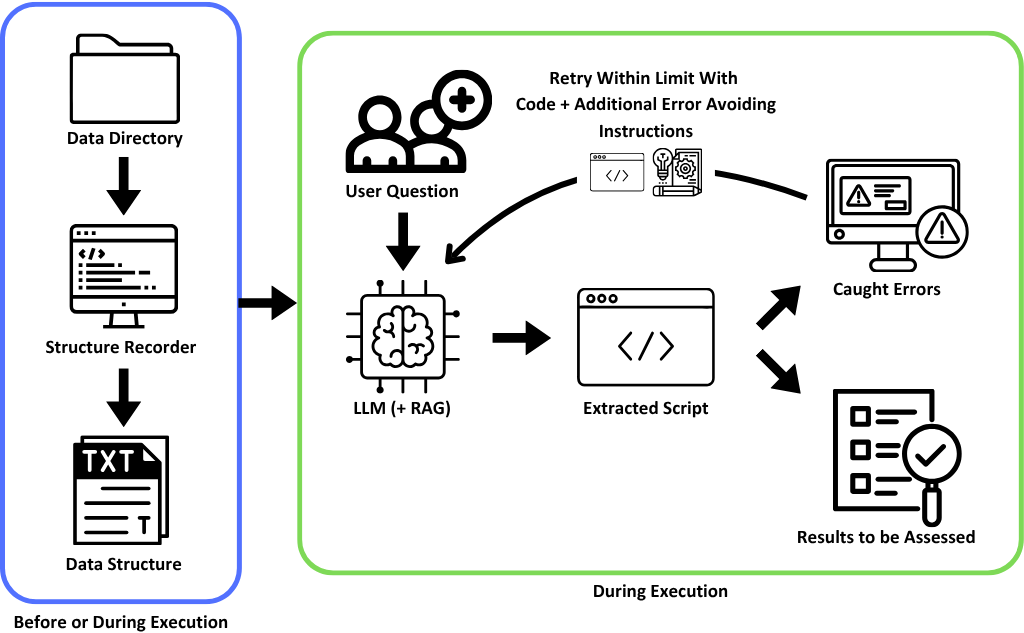
\includegraphics[width=0.85\linewidth]{img/Methodology/Experiment Workflow.png}
    \caption[Overview of experiment architecture]{\textbf{Overview of experiment architecture}. 
    First, the data directory is analyzed, and the structure recorder extracts the data structure into a text file. This is integrated into the LLM (+RAG) system, which retrieves relevant context before generating a response. Upon receiving a user question, the model generates code to answer it. The script is extracted, executed, and upon success, its results are assessed. If errors occur, they are caught, appended to the prompt alongside the generated code, and the model retries within a set limit before halting if issues persist.}
    \label{fig:experiment_architecture}
\end{figure}

This experiment explores an LLM-based approach for intelligent and adaptive data analysis on DDPs. A simplified overview of this experiment can be observed in Figure~\ref{fig:experiment_architecture}. The system builds on an existing codebase and begins by generating a textual representation of the DDP's structure via an LLM-generated Python script. This information is integrated into the knowledge base in the RAG variant or provided to the model via prompts. As such, it compares a standard LLM setup with a RAG-enhanced variant to address context window limitations and assess the two approaches.

\section{Pipeline Overview}

This experiment builds upon an existing application developed by Jonathan Decker, which implements a minimal RAG system using Chat AI~\cite{doosthosseini2024chataiseamlessslurmnative} services. The original codebase\footnote{\url{https://gitlab-ce.gwdg.de/hpc-team-public/chat-ai-llamaindex-examples}} provides a framework for sending API service requests to any model listed under Chat AI.

\subsection{Structure Recorder}

As shown in Figure~\ref{fig:structure_recorder}, the data structure of the DDP is integrated into the project's knowledge base using a structure recorder script. This Python script, generated by GPT-4o Mini~\cite{gpt-4o}, recursively traverses the directory structure of an exported data folder. During this process, the script captures the hierarchy of all nested folders and files, as well as the internal structure of any encountered JSON files. At its core, it constructs a nested dictionary representing the folder and file organization, with special handling for some JSON and image files.

\begin{figure}[h]
    \centering
    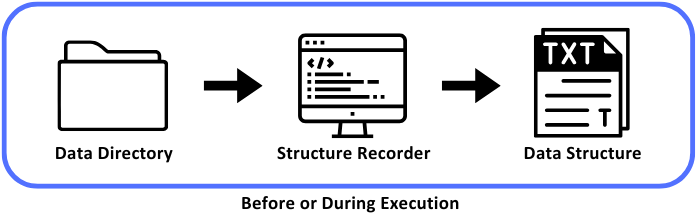
\includegraphics[width=0.70\linewidth]{img/Methodology/Structure Recorder.png}
    \caption[Structure recorder workflow]{\textbf{Structure recorder workflow}. Simplified visualization of the structure recording script that generates a textual file containing the directory hierarchical structure along with the structure of all the relevant JSON objects and files.}
    \label{fig:structure_recorder}
\end{figure}

The complete hierarchical organization of the directory is recorded in order to provide the model with additional task-related contextual information. For instance, when answering questions related to advertisements, the model is expected to search within the \emph{ads\_information} directory.  Furthermore, this structure informs the model about the exact location of each file, so that the model knows exactly where to look for the files it deems relevant to the answer of the given query.

For each JSON file, the script loads its content and extracts its structural schema (i.e., key-value patterns and nested object types) using a recursive function. A notable exception is the inbox directories, which typically contain multiple subfolders, each representing individual conversations or parts of them. Instead of recording every message in every conversation, the script selects the conversation folder with the most diverse message structures and summarizes only that one, avoiding redundancy. In addition, no JSON values are recorded throughout this process. Instead, they are replaced by the data type of the corresponding field.

The names of the conversation folders are anonymized to \emph{username\_placeholder} to preserve privacy. Additionally, all \emph{.jpg} files are generalized and recorded just as \emph{image.jpg}, regardless of their original filename. These precautions and refinements are implemented in order to prevent the recording and exposure of sensitive data to the models. Due to the deep and highly complex nature of some DDPs, other data in these directories may be considered sensitive but have not been identified or handled by us. Therefore, future researchers are advised to proceed with caution when trying a similar approach to this structure recorder.

The final resulting structure is saved as a formatted JSON string into a textual file, providing a clean, structured overview of the data archive for documentation or analysis purposes. The generated data structure file looks like the following snippet in Figure~\ref{fig:data_structure_snippet}. The performance of the chosen LLMs, using this file as context for generation, is indirectly contributing to addressing \textbf{RQ1}.

\subsection{Codebase}

For each conducted experiment, the same pipeline is executed, consisting of the following steps. For every predefined data query, we iterate through all the chosen LLMs. For each model, we then apply the query across the collected DDPs. In each experimental instance, we log the model's performance, the generated code, and any errors encountered during code execution. When an error occurs, the original code and its corresponding error message are appended to the prompt, accompanied by corrective instructions that inform the model of the faulty behavior in its output. This updated prompt is then resubmitted to the model for a retry attempt, with retries capped at a maximum limit of five. Alongside the evaluation logs, all code that is generated during the experiment is also recorded. All experimental records and the codebase are publicly available in our repository\footnote{\url{https://github.com/miger-shkrepa/adaptive-donated-data-analysis}}.

\section{Model Selection and Setup}

To fairly evaluate the feasibility of this approach, open source language models are chosen from diverse providers, varying in size and instruction tuning. This allows us to assess which combinations of scale and training are most effective for the task at hand, and whether instruction-specific fine-tuning or model size has a noticeable impact on performance. You can refer to Table~\ref{tab:llm_overview} for an overview of these models.

\begin{table}[ht]
\centering
\small
\begin{tabular}{l l c c l}
\toprule
\textbf{Model} & 
\textbf{Developer} &
\makecell{\textbf{Parameter} \\ \textbf{size}} &
\textbf{Reference} \\
\midrule
Llama3.1 8B Instruct       & Meta        & 8B   &~\cite{grattafiori2024llama3herdmodels} \\
Codestral 22B Instruct     & Mistral        & 22B   &~\cite{codestral} \\
Qwen2.5 Coder 32B Instruct & Alibaba Cloud   & 32   &~\cite{qwen2} \\
Llama3.1 70B Instruct      & Meta        & 70B  &~\cite{grattafiori2024llama3herdmodels} \\
Qwen2.5 72B Instruct       & Alibaba Cloud   & 72B  &~\cite{qwen2} \\
Mistral Large Instruct     & Mistral        & 123B  &~\cite{largemistral} \\
\bottomrule
\end{tabular}
\caption[Overview of selected LLMs]{\textbf{Overview of selected LLMs}. Some of the key technical attributes on the chosen models, along with the organizations behind their development, and references to the relevant technical reports or model documentation.}
\label{tab:llm_overview}
\end{table}

\subsection{LLM Access and Interaction Setup}

The employment and usage of all the aforementioned models are made easily accessible and remotely available to this research through the Chat AI platform. This web service provides secure access to several commercial LLMs. It does not store user or conversation data, which aligns with the privacy requirements of this research, as DDPs may contain sensitive information. Communication with the models is facilitated via API requests using the OpenAILike wrapper~\cite{openai_like}, which enables easy configuration of various model parameters such as temperature, context window, and the maximum number of generated tokens. This wrapper also allows for querying the models via Python scripts, making it possible to run this experiment on our local machines. 

Due to the large size and high demand of some models, particularly Llama3.1-70B, the response times could be substantial. This model occasionally exceeded the API service timeout limit and resulted in experimental failure. To mitigate these delays and timeout constraints, some requests to Llama3.1-70B near the end of the experiment were routed through the NVIDIA API service\footnote{\url{https://build.nvidia.com/meta/llama-3_1-70b-instruct}} using the same wrapper. It is important to note that the RAG functionality used in this study is only supported via the Chat AI API service and not the NVIDIA one. Additionally, the RAG pipeline employs E5 Mistral 7B Instruct~\cite{wang2024improvingtextembeddingslarge} for embedding.

\subsection{Parameter Configuration}

\begin{table}[ht]
\centering
\small
\begin{tabular}{l p{8cm} l p{1.1cm}}
\toprule
\textbf{Parameter} & \textbf{Description} & \textbf{Default} & \textbf{Set} \\ & & \textbf{Value} & \textbf{Value} \\
\midrule
temperature & Raising the temperature setting encourages the model to produce more inventive responses. In the context of code generation, this can lead to the introduction of new libraries, the use of custom method and function names, restructured code, and occasionally incomplete outputs~\cite{deshpande2025retrieval}. & \texttt{0.1} & \texttt{0} \\
\midrule
is\_chat\_model & Indicates whether the model uses a chat-based or plain text completion endpoint~\cite{openai_like}. & \texttt{False} & \texttt{True} \\
\midrule
context\_window & This determines the size of the context window, i.e., the upper limit of tokens the model can process while generating a response~\cite{openai_like}. & \texttt{3900} & \texttt{3900; \newline 50000} \\
\bottomrule
\end{tabular}
\caption[Modified API configuration parameters]{\textbf{Modified API configuration parameters}. The table lists the OpenAILike API parameters that were adjusted for this experiment, including their descriptions, default values, and the values used.}
\label{tab:api_config_params}
\end{table}

The OpenAILike API service allows for the configuration of several parameters that impact the model's generation and response behavior. Table~\ref{tab:api_config_params} lists the parameters adjusted for this experiment along with their chosen values. 

\emph{Temperature} is reported to be one of the most influential parameters in LLMs' generating performance~\cite{arora2024optimizinglargelanguagemodel}. 
As such, we set the parameter to zero, as using low temperatures (below 0.5) is more effective for code generation tasks~\cite{arora2024optimizinglargelanguagemodel,10.1145/3697010}. Moreover, setting it to zero yields more deterministic and consistent outputs~\cite{10.1145/3697010}. The \emph{is\_chat\_model} parameter is set to true, enabling a conversation-based generation between the model and the user. The system message, i.e., the model's behavior and formatting style, has not been modified and remains the default \enquote{You are a helpful assistant}. Regarding the \emph{context\_window} parameter, two experimental phases are conducted. The first phase focuses on the RAG implementation and evaluation, during which the context window is set to the default value of 3,900 tokens. In the second phase, where the focus shifts to experimenting with prompt-only instructions, the token limit is adjusted based on the size of the supplemental data and increased to 50,000 tokens.

\subsection{Prompt Structure and Design}

Engineering effective prompts plays a vital role in guiding LLMs to generate relevant and high-quality outputs~\cite{10.1007/978-981-99-7962-2_30}. When developers and information seekers understand how to construct well-designed prompts, they can enhance model performance and adapt to different domains~\cite{10.1007/978-981-99-7962-2_30}. Interviewed experts also highlight that high-quality prompts help steer the model toward more accurate and purposeful responses, especially when providing a considerable amount of context~\cite{simon2023promptguidelines}.
LLMs can operate under different prompting configurations, adapting to instructions without or through fine-tuning~\cite{naveed2024comprehensiveoverviewlargelanguage}.
Prompt engineering is considered a lightweight form of programming, allowing users to tailor the behavior and output of the model to meet specific needs and use cases~\cite{10.1007/978-981-99-7962-2_30}. It also allows for the integration of diverse prompting strategies, enhancing the quality of LLM outputs and promoting knowledge exchange between developers and information seekers~\cite{10.1007/978-981-99-7962-2_30}. This supports building more advanced applications, deepens understanding of model behavior, and helps guide LLMs toward producing truthful and informative responses~\cite{10.1007/978-981-99-7962-2_30}.

To ensure the generated Python code is suitable for remote execution and consistent evaluation, we design a structured base prompt that enforces a series of generation rules. These rules guide the model to produce code that is robust and compatible with our local execution environment. The prompt outlines key expectations such as input handling, error management, and output formatting, while explicitly restricting the use of non-standard libraries. Since the user queries do not inherently require advanced functionalities beyond what the standard Python library offers, relying solely on built-in modules allows for a more direct and impartial comparison of the models' reasoning and problem-solving capabilities. By clearly defining how the input path should be referenced, how exceptions should be raised, and how output should be structured, we ensure that all generated scripts are not only syntactically correct but also aligned with the broader goals of automation, evaluation, and comparison across models. 

Additionally, while the core structure of the prompt remains fixed across all experiments, the final instruction is adapted based on the specific design details for each experiment. This last rule determines how the model should interpret the completeness or reliability of the dataset and how it should behave when encountering uncertainty or missing information. It allows us to simulate a range of realistic use cases, from degradation under missing data conditions to autonomous reasoning and data exploration. For more details on the experimental setups, refer to Section~\ref{experimental_setup}. The base prompt structure can be found in Figure~\ref{fig:query_instructions}.

\section{Evaluation}

\subsection{Dataset Overview}

\begin{figure}[!b]
    \centering
    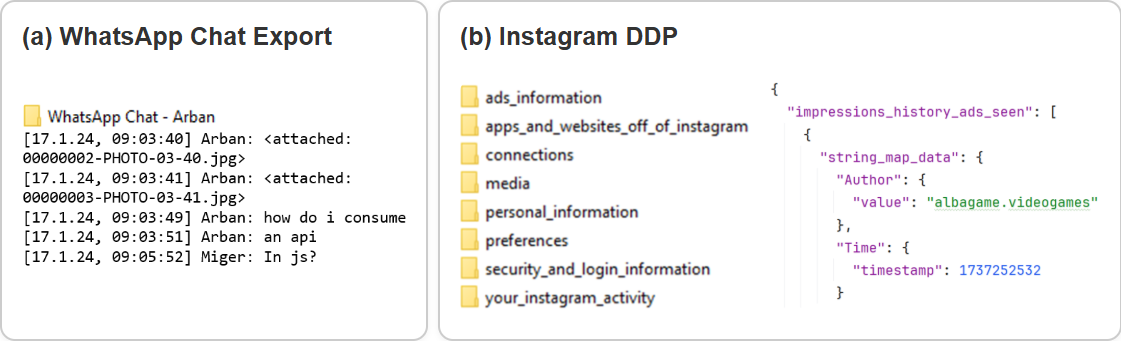
\includegraphics[width=1\linewidth]{img/Methodology/structure-comparison.png}
    \caption[Comparison of digital trace structures]{\textbf{Comparison of digital trace structures}. WhatsApp (a) issues text-based logs organized by conversation, which include timestamps, participant names, and message content. Instagram DDPs (b) consist of highly structured JSON data captured across several of its application features and organized into multiple folders and subdirectories.}
    \label{fig:structure_comparison}
\end{figure}

Different applications, websites, and domains focus on different forms of data to collect and analyze. As a result, data controlling entities issue DDPs that vary greatly in structure, content, and scope of information captured. The structural and complexity differences between the DDPs issued by WhatsApp and Instagram can be observed in Figure~\ref{fig:structure_comparison}. For this research, we select Instagram-issued DDPs as the primary dataset for evaluation. After a thorough analysis, we recognize these DDPs as highly complex, deeply structured, and extensive in size, making them an ideal candidate for this assessment. The richness and diversity of Instagram's data present a robust challenge that effectively tests the capacity of LLMs to navigate nested structures and varied formats of complex real-world data, comprehend them, and extract meaningful information. This also ensures that the evaluation directly captures the models' practical abilities in handling large-scale, multifaceted data, an inherently difficult task typical of modern digital environments.

Thirteen DDPs are collected from different individuals, each reflecting data spanning distinct periods. To evaluate the models' ability to handle missing data and introduce variation in the analysis, some of the examined packages capture only a subset of the data scope that Instagram typically records. As a result, the volume of the collected data varies widely, with some occupying only a few kilobytes, whereas others extend into the hundreds of megabytes or even exceed a gigabyte. This also simulates real-world scenarios, where users may not be willing to submit all of their data due to privacy concerns or personal preferences. 

While investigating these packages, we observe how Instagram manages data recording and collection. Since they collect data across several features they offer, if an individual has not interacted with a particular feature, Instagram does not create the relevant JSON file or folder corresponding to said feature. In some cases, they create a no-data text file inside the relevant JSON folder as a placeholder instead. The models must correctly handle missing files or directories where data would normally be found, avoid errors, and generate code that adapts to such situations.

\subsection{Data Queries and Response Structure}

Regarding the user queries for the LLMs, in the initial phases of the experiment, we consulted with a researcher who frequently works with Instagram DDPs to gain insights into how these questions are typically formulated, what types of information they are intended to retrieve, and what data domain these queries pertain to. The first three queries used in this experiment were provided by this researcher and are structured as follows:

\begin{figure}[ht]
    \centering
    \fbox{%
        \begin{minipage}{0.95\linewidth}
        \begin{enumerate}
            \item What topics does Instagram determine to be of interest for a user?
            \item How often does a user see advertisements and about which topics (from which companies)?
            \item How often do people see posts (daily and weekly)?
        \end{enumerate}
        \end{minipage}
    }
\end{figure}

Building on these initial three queries as a template, nine additional questions were developed to capture information across different features of Instagram. It is important to note that all of the designed queries are strictly quantitative in nature, capturing information that requires only mathematical operations when organized into a response. When constructing these questions, we aimed to maintain a degree of impartiality and minimize any direct correlation between the phrasing of the question and the exact data structure belonging to the answer. The queries are also designed to increase in complexity, with the first ones targeting information that is directly retrievable from JSON objects. Subsequent queries require the model to perform aggregation or structural reorganization of the retrieved data, and the final set of questions calls for cross-referencing information from multiple JSON files and subdirectories. It is up to the model to interpret the natural language instructions and correctly retrieve, combine, and format the necessary data accordingly. When designing these queries, only questions that could be answered using the provided data were considered, ensuring that the evaluation remains grounded in what the DDPs actually contain. The complete list of queries used in this experiment is presented in Figure~\ref{fig:used_queries}.

To ensure that all models' responses are compatible with a shared evaluation methodology, specific query instructions are designed for each question. These instructions define a strict response structure, requiring the output to be formatted as a CSV file with a predefined column arrangement. For the first three data queries, the corresponding query instructions are as follows:

\begin{figure}[ht]
    \centering
    \fbox{%
        \begin{minipage}{0.95\linewidth}
        \begin{enumerate}
            \item The response must be a structured CSV file with one column: Topics of Interest.
            \item The response must be a structured CSV file with two columns: Company Name and Number of Ads Viewed.
            \item The response must be a structured CSV file with three columns: Date/Week, Posts Viewed and Type. The 'Type' column must contain either 'Daily' or 'Weekly' as values. The 'Date/Week' Column must follow the 'YYYY-MM-DD' format (e.g., 2025-01-18) for daily dates and the 'Week YYYY-WW' format (e.g., Week 2025-02) for weeks. The weekly value must be generated using strftime('\%Y-\%W'), where weeks start on Monday.
        \end{enumerate}
        \end{minipage}
    }
\end{figure}

For the first two queries, relatively simple instructions are provided, specifying the names and expected number of columns in the response CSV files. The third query involves temporal data and thus requires more comprehensive instructions, including specific formatting rules and illustrative examples. These ensure that the models adhere to the correct format, particularly in terms of date representations. The same formatting principles apply to the remaining queries, with additional constraints or clarifications introduced as necessary to accommodate more complex data retrieval or structuring requirements. The complete set of query response instructions is provided in Figure~\ref{fig:query_response_instructions}.

\subsection{Baseline}

To establish a basis for comparison, we utilize two larger, state-of-the-art language models: OpenAI's GPT-4o Mini and Deepseek-V3~\cite{deepseekai2025deepseekv3technicalreport}. These models are selected based on their accessibility, strong performance in recent benchmarks~\cite{puspitasari2025deepseek,gao2025comparisondeepseekllms}, and strong position in the current AI landscape. 

These models serve a practical role in navigating the complexity of the Instagram DDP. The structure of these DDPs, spread across deeply nested directories and diverse JSON schemas, makes it significantly difficult for us to manually establish ground truth answers for every query, especially for those requiring cross-referencing across multiple files. Instead, we leverage the outputs of these two models. Each of them is provided with the same structure text file, prompt, and user query to ensure consistency. The code generated from them and the corresponding CSV file are thoroughly analyzed and validated manually against the directory structure in terms of relevance and accuracy. Upon establishing confidence in the response and deciding on the more accurate one between the two models, the CSV response for each query serves as a benchmark to evaluate the accuracy of the experimented models. This benchmarking process is conducted only once. It is important to note that Deepseek-V3 and GPT-4o Mini are not part of the following evaluation steps. Their role is limited to providing the reference responses used to assess accuracy.

\section{Evaluation Metrics} \label{evaluation_metrics}

To provide a comprehensive assessment, our analysis is structured around three evaluation domains: performance metrics, error analysis, and code evaluation. Together, these dimensions offer a multifaceted view of each model's capabilities, measuring how reliable their outputs are and also how robust their generated code is. Performance evaluation focuses on correctness, while error analysis investigates the patterns of runtime failures, identifying key areas where models tend to struggle. Lastly, code evaluation provides insights into the complexity and documentation patterns of the generated scripts using established software metrics, all computed via the Radon Python library. For each experimental instance, all of these domain metrics are recorded with a UUID, ensuring traceability of the results and cross-log relation. All metrics and recorded outputs in this section contribute directly to answering \textbf{RQ2}.

\subsection{Performance Metrics} \label{performance_metrics}

To evaluate the accuracy of the selected models, we focus on the structure of the responses, which are formatted as CSV files with predefined columns for each query. We define three key attributes for this comparison (see Table~\ref{tab:csv_comparison}):

\begin{enumerate}
    \item \textbf{Correct Rows} — Rows that are present in both the ground truth CSV file and the model-generated CSV file, representing correctly retrieved information.
    \item \textbf{Missing Rows} — Rows that exist in the ground truth CSV but not in the generated file, indicating information the model failed to retrieve due to faulty logic, incomplete parsing, or implementation errors.
    \item \textbf{Extra Rows} — Rows that appear in the generated CSV file but not in the ground truth, reflecting irrelevant information retrieved by the model, often due to overestimation of the response or misinterpretation.
\end{enumerate}

\begin{table}[ht]
    \centering
    \setlength{\arrayrulewidth}{0.3mm}
    \renewcommand{\arraystretch}{1.3}
    \begin{tabular}{|>{\columncolor{white}}l r!{\vrule width 1.2pt}>{\columncolor{white}}l r|}
    \hline
    \multicolumn{2}{|c!{\vrule width 1.2pt}}{\textbf{Ground Truth CSV}} & \multicolumn{2}{c|}{\textbf{LLM Generated CSV}} \\
    \hline
    \textbf{Company} & \textbf{Ads Viewed} & \textbf{Company} & \textbf{Ads Viewed} \\
    \hline
    temu     & 7 & \cellcolor{green!20} temu      & \cellcolor{green!20} 7 \\
    apple    & 1 & \cellcolor{yellow!20} Mannheim  & \cellcolor{yellow!20} 3 \\
    \cellcolor{red!15} airbnb   & \cellcolor{red!15} 4 & \cellcolor{yellow!20} Frankfurt & \cellcolor{yellow!20} 4 \\
    \cellcolor{red!15} google   & \cellcolor{red!15} 2 & \cellcolor{green!20} apple     & \cellcolor{green!20} 1 \\
    \hline
    \end{tabular}
    \caption[Comparison between ground truth and LLM-generated results]{\textbf{Comparison between ground truth and LLM-generated results}. Green rows indicate correct matches (True Positives), red rows represent missing entries (False Negatives), and yellow rows denote unexpected extra entries (False Positives).}
    \label{tab:csv_comparison}
\end{table}

In this analysis, as illustrated in Table~\ref{tab:confusion_matrix}, \textbf{Correct Rows} are treated as \emph{True Positives} (TP), \textbf{Missing Rows} as \emph{False Negatives} (FN), and \textbf{Extra Rows} as \emph{False Positives} (FP). In our CSV comparison process, row order is disregarded entirely. Instead, each row is treated as a unique combination of values across all columns, and comparison is based solely on content rather than position. To ensure consistency, all CSV values are normalized by trimming redundant spaces, converting text to lowercase,  standardizing data types (e.g., converting 5 to 5.0), and standardizing encodings (e.g., accents or Unicode variants) to avoid superficial mismatches. This ensures a position-independent and content-driven comparison, ideal for structured data validation.

Based on these categories, we compute the following standard evaluation metrics:

\begin{itemize}
    \item[] – \textbf{Precision}: Measures the accuracy of the model's positive predictions.

    \begin{equation}
        \text{Precision} = \frac{TP}{TP + FP}
    \end{equation}
    
    \item[] – \textbf{Recall} (Sensitivity): Indicates the proportion of actual positive instances that the model correctly retrieved.

    \begin{equation}
        \text{Recall} = \frac{TP}{TP + FN}
    \end{equation}
    
    \item[] – \textbf{F1 Score}: The harmonic mean of precision and recall, providing a balanced metric that balances the importance of the two and accounts for both false positives and false negatives. 

    \begin{equation}
        F1 = 2 \cdot \frac{\text{Precision} \cdot \text{Recall}}{\text{Precision} + \text{Recall}}
    \end{equation}
    
\end{itemize}

\begin{table}[h]
    \centering
    \renewcommand{\arraystretch}{1.3}
    \begin{tabular}{@{}lcc@{}}
    \toprule
     & \textit{Predicted Positive} & \textit{Predicted Negative} \\
    \midrule
    \textit{Actual Positive} & True Positive (TP) & False Negative (FN) \\
    \textit{Actual Negative} & False Positive (FP) & True Negative (TN) \\
    \bottomrule
    \end{tabular}
    \caption[Structure of a binary confusion matrix]{\textbf{Structure of a binary confusion matrix}. Table adapted from~\cite{vujovic2021classification}. Outline of the standard layout used in binary classification tasks, highlighting the relationships between predicted and actual outcomes.}
    \label{tab:confusion_matrix}
\end{table}

Since we are employing LLMs for this task, it is expected that repeated executions of the same prompt do not always yield identical outputs. As such, some degree of variability and fluctuation in model behavior and output is anticipated. To capture and quantify this dispersion, \emph{variance} and \emph{standard deviation} are used:

\begin{itemize}
    \item[] – \textbf{Variance}: Measures how far each value in a dataset deviates from the mean, indicating the overall spread of the data.

    \begin{equation}
        s^2 = \frac{1}{n} \sum_{i=1}^{n} (x_i - \bar{x})^2
    \end{equation}
    
    \item[] – \textbf{Standard Deviation}: Represents the square root of the variance and describes how much variation or dispersion there is in a set of data points.

    \begin{equation}
        \sigma = \sqrt{\operatorname{Var}(x)}
    \end{equation}
\end{itemize}

In our evaluation, we track both the standard metrics and key row classification counts to allow for a deeper investigation into instances of severely low performance. Additionally, we collect other information relevant to performance, such as the number of retries required for a model to produce an executable response. This allows us to identify which models tend to struggle with the code generation for this task and from which models to expect executable code on the first attempts. We also record the duration of each experimental instance to provide insights into the relative response speed from different models. While this metric is inherently biased by the infrastructure and throughput of the two API services employed in this study, it still offers valuable context, especially given the reputations and performance expectations associated with some of the evaluated models. 

For each record, we also log the associated DDP, the specific data query, and the model used. This enables further analysis of individual results and supports detailed comparisons across models and scenarios. Since some DDPs may only contain a subset of the complete Instagram data, specific queries may not be answerable due to missing information. To account for this, we explicitly track whether a given DDP contains the necessary data to produce a valid response. This allows for additional insights into the models' ability to handle incomplete or missing data.

Given that in some instances, there is no available answer data for some of the queries across specific DDPs, an interesting evaluation challenge is introduced. Theoretically, when no relevant answer data exists for a given query, the correct behavior would be for the model to produce an empty CSV file. If the model generates code that, upon execution, creates an empty CSV file under these conditions, it is considered a successful outcome. As such, for these instances, a precision, recall, and F1 score of 1 is assigned.

However, complications arise when a model generates an empty CSV file due to faulty code. In such cases, although the output matches the expected result, it is not functionally correct. For this reason, the performance evaluation is mostly focused on the models' results on complete data packages. 

As for scenarios involving incomplete data, the code generated under these experimental conditions is re-executed on a complete dataset, allowing us to classify models that can produce valid logic correctly. This labeling is based on comparing executions on the datasets with and without the necessary data (see Table~\ref{tab:nodata_classification}).  If a model produces an empty response on the dataset without data but generates a complete or partially accurate output on the dataset with data, it can handle missing data. If it generates an empty response on both datasets, it gets labeled as faulty logic, as the code always produces empty files. If the model produces a non-empty output on the dataset without data, it indicates an incorrect model, as it generates extra rows, suggesting it is looking at the wrong files for an answer. Finally, if execution fails on the dataset without data, it is not re-executed, and the instance is labeled as failed.


\begin{table}[ht]
    \centering
    \renewcommand{\arraystretch}{1.2}
    \setlength{\tabcolsep}{12pt}
    \small
    \begin{tabular}{c c c}
    \toprule
    \multicolumn{2}{c}{\textbf{F1 Score on Dataset}} & \multirow{2}{*}{\textbf{Label}} \\
    \cmidrule(lr){1-2}
    \textbf{Without Data} & \textbf{With Data} & \\
    \midrule
    1 & $0 < F1 \leq 1$ & Correct \\
    \rowcolor{gray!10} 
    1 & $0$ & Faulty Logic \\
    0 & $F1 \geq 0$ & Incorrect \\
    \rowcolor{gray!10} 
    \textit{null} &  & Failed \\
    \bottomrule
    \end{tabular}
    \caption[Classification scheme for evaluating model performance on handling missing data]{\textbf{Classification scheme for evaluating model performance on handling missing data}. Generated code is executed on datasets without the necessary data and on those with it. Results are then compared across the two datasets to identify model performance.}
    \label{tab:nodata_classification}
\end{table}

If a model fails to generate executable code within the designated retry limit, all of the mentioned metrics and row classification values are recorded as \emph{null} in the instance log. This serves as an indicator that the model was unable to provide a valid response for that experimental instance. In cases where a timeout error occurs and the API request is aborted, no data is recorded for that attempt. Instead, the failed instance is manually retried until a valid response is obtained, after which the evaluation and pipeline proceed as usual.

\subsection{Error Analysis}

The code generated by the selected models is expected to produce runtime errors occasionally. To address this, error handling and formatting instructions are introduced in the base prompt. Whenever an error is caught during the execution of the generated code, the execution is aborted, and the runtime error is logged for later analysis. Each error log captures the type of error that occurred and its associated message, which facilitates preprocessing and categorization. Additionally, we record the attempt number at which the error occurs, allowing us to identify persistent error types and which models struggle most with specific categories of runtime issues.

\begin{table}[ht]
    \centering
    \small
    \begin{tabular}{p{2.3cm}|p{5.7cm}|p{5.7cm}}
    \toprule
    \multicolumn{1}{c|}{} & \multicolumn{1}{c|}{\textbf{Rule-Based Pattern Matching}} & \multicolumn{1}{c}{\textbf{Keyword Similarity Matching}} \\
    \midrule
    \midrule 
    \textbf{Error Message} & \textbf{No such file or directory}: 'data.csv' & \emph{'list' object has} no attribute 'get' \\
    \midrule
    \textbf{Original Label} & UnknownError & UnknownError \\
    \midrule
    \textbf{New Label} & FileNotFoundError & AttributeError \\
    \midrule
    \midrule 
    \textbf{Error Message} & \textbf{'charmap' codec} can't encode character... & Error: Unable to parse login time. \\
    \midrule
    \textbf{Original Label} & UnknownError & UnknownError \\
    \midrule
    \textbf{New Label} & UnicodeEncodeError  & UnknownError \newline (not matched to any known template) \\
    \bottomrule
    \end{tabular}
    \caption[Examples of automated error reclassification]{\textbf{Examples of automated error reclassification}. Rule-based and keyword-similarity approaches are applied to unknown errors. \textbf{Bold} text highlights matched patterns, while italic text indicates frequently occurring keywords (with a minimum keyword frequency threshold of three).}
    \label{tab:automated_error_reclassification}
\end{table}

This approach does introduce some bias regarding the nature of the recorded errors, as they are expected to reflect issues typical of data retrieval and analysis tasks. We assume the models attempt to anticipate the issues they consider are more likely to occur and raise exceptions accordingly. However, in some cases, errors are caught under a generic exception clause that does not attribute any error type. For these instances, the error type is automatically labeled as \emph{Unknown Error}, while the error message is still recorded as usual. To refine the categorization of these cases, we perform preprocessing steps aimed at reclassifying mislabeled or ambiguous entries based on their error messages (see Table~\ref{tab:automated_error_reclassification}).

First, we attempt to reclassify errors labeled as \emph{Unknown Error} that specifically belong to the \emph{FileNotFoundError} category. This is done by checking whether the associated error message contains specific phrases such as \enquote{file does not exist} or \enquote{No such file or directory}.

In the second step, we apply a combination of rule-based pattern matching and keyword-based similarity analysis. Similarly to the first step, specific rules are used to detect common error patterns and assign the appropriate labels of \emph{InvalidTimeStampFormat}, \emph{UnicodeEncodeError}, and \emph{DataNotFoundError}, based on the content of the error message. For the remaining unknown errors, frequently occurring keywords from previously labeled error types are extracted to create reference templates. If the message of an unknown error shares at least three keywords with any of these templates, the error is reclassified accordingly.

The result of this process is a cleaned and more accurately labeled error dataset, which is stored in a new CSV file for further analysis. As a final step, we manually review this file to identify and correct any misclassifications based on the content of the error messages. We also assign appropriate labels to any remaining \emph{Unknown Error} entries that were not captured during the automated preprocessing, using the same rule-based methodology applied earlier.

\subsection{Code Analysis}

While LLMs can enhance productivity by rapidly generating code, findings highlight the importance of evaluating the code before integrating it into production systems~\cite{licorish2025comparinghumanllmgenerated}. Ideally, such code would be assessed based on functional correctness by running it against elaborate test cases~\cite{farchi2024automaticgenerationbenchmarksreliable}. However, this approach is only feasible for simple tasks that do not require a comprehensive testing infrastructure~\cite{farchi2024automaticgenerationbenchmarksreliable}. As a result, most evaluation methods rely on reference-based metrics that compare the generated output to a known ground truth~\cite{farchi2024automaticgenerationbenchmarksreliable}.

In our evaluation schema, each instance of successfully executable code is recorded and evaluated. It is important to emphasize that the coding analysis metrics utilized are not used to assign an absolute score to each model's programming skills. Instead, they are employed to compare generated code across models, offering insights into their differences and what to expect from them in terms of code readability and understandability. All evaluation metrics are calculated using the Radon~\cite{radon} Python library and are defined as follows:

\paragraph{Cyclomatic Complexity}\mbox{}\\

\noindent Cyclomatic Complexity~\cite{1702388} is used to count the number of independent decision paths within a program, serving as a measure of code complexity~\cite{takerngsaksiri2025codereadabilityagelarge}. This metric is commonly used to assess the testability and maintainability of software~\cite{licorish2025comparinghumanllmgenerated}, as higher cyclomatic complexity is often associated with a greater likelihood of errors and bugs~\cite{10507163}. Formally, it is defined as:
\begin{equation}
        C = D + 1
\end{equation}
where $D$ is the number of decision points in the code~\cite{takerngsaksiri2025codereadabilityagelarge}. Elements such as conditional branches, loops, boolean operations, and exception handling all contribute to this count.

The Radon library calculates cyclomatic complexity at the function level, generating a list of complexity scores for each function in the script. As a result, code that contains only top-level logic without any function definitions may be ignored or not evaluated properly. To address this, our script first checks whether the generated code contains any function blocks. If none are found, the code is wrapped in a synthetic global function to ensure complexity evaluation. During evaluation, we track both the maximum cyclomatic complexity, representing the most complex individual function, and the total cyclomatic complexity, which aggregates the complexity of all decision structures across the script. The former highlights the most intricate logic block, while the latter reflects the overall control-flow complexity of the generated code and the total logic burden.

\paragraph{Raw Metrics}\mbox{}\\

\noindent In addition to cyclomatic complexity, our evaluation also considers various code size metrics computed by the Radon library. These metrics help quantify the structural composition of the generated scripts~\cite{radon}:

\begin{itemize}
\item LOC: The total number of lines in the code. This may differ from the actual number of lines in the file due to parsing behavior.
\item LLOC: The number of logical statements in the code, where each line corresponds to a single executable statement.
\item SLOC: The number of source lines, not necessarily corresponding to the LLOC.
\item Comments: The number of lines containing comments. Note that multi-line strings are not considered comments, as they are interpreted as regular strings in Python.
\item Multi: The number of lines occupied by multi-line string literals.
\item Single Comments: The number of lines that are just comments with no code.
\item Blanks: The number of blank or whitespace-only lines.
\end{itemize}

Using these metrics, the comment ratio of each script can also be calculated, defined as the percentage of comments to LOC. As comment density is subjective and context-dependent~\cite{10.1145/3338906.3342494}, we use it exclusively to compare the models to one another.

\paragraph{Halstead Metrics}\mbox{}\\

\noindent Halstead Metrics~\cite{10.5555/540137} are a set of metrics designed to quantify various aspects of code~\cite{takerngsaksiri2025codereadabilityagelarge} and the relations between them~\cite{radon}. These metrics are among the earliest measures of program complexity, and several authors consider the suite controversial due to its underlying psychological assumptions about code~\cite{bucur2006quality}. The main mathematical formulas are derived from basic code properties such as the number of operators and operands, but they do not take the code's meaning or context into consideration~\cite{bucur2006quality}. As such, Halstead metrics offer a descriptive analysis of code complexity, but lack a prescriptive component to guide developers on how to address or improve identified issues~\cite{bucur2006quality}. Despite these limitations, Halstead metrics have been widely applied over the past three decades in areas such as fault prediction, software quality assessment, and similarity analysis~\cite{bucur2006quality, khan_evaluating_2023}. These metrics are employed to evaluate key attributes using the following measures:

\begin{itemize}[noitemsep, topsep=0pt]
\item $h_1$:  the number of distinct operators.
\item $h_2$: the number of distinct operands.
\item $N_1$: the total number of operators.
\item $N_2$: the total number of operands.
\end{itemize}

\noindent Based on these notations, the following formulas are used in our evaluation:

\begin{itemize}
  \item \textbf{Program Vocabulary}: the number of unique operators and operands.
    \begin{equation}
        h = h_1 + h_2
    \end{equation}
  \item \textbf{Program Length}: total number of operators and operands.
    \begin{equation}
        N = N_1 + N_2
    \end{equation}
  \item \textbf{Calculated Program Length}: theoretical minimum length for the code.
    \begin{equation}
        \hat{N} = h_1 \log_2 h_1 + h_2 \log_2 h_2
    \end{equation}
  \item \textbf{Volume}: size of the program based on length and vocabulary size.
    \begin{equation}
        V = N \log_2 h
    \end{equation}
  \item \textbf{Difficulty}: the difficulty of the program to modify or understand.
    \begin{equation}
        D = \frac{h_1}{2} \cdot \frac{N_2}{h_2}
    \end{equation}
  \item \textbf{Effort}: mental effort required to implement or understand the code.
    \begin{equation}
        E = D \cdot V
    \end{equation}
  \item \textbf{Time Required to Program}: estimated time for implementation (in seconds).
    \begin{equation}
        T = \frac{E}{18 \text{ seconds}}
    \end{equation}
  \item \textbf{Estimated Number of Delivered Bugs}: estimated number of bugs in the code.
    \begin{equation}
        B = \frac{V}{3000}
    \end{equation}
\end{itemize}

\paragraph{Maintainability Index}\mbox{}\\

\noindent The Maintainability Index~\cite{242525} is a software metric typically used to measure how maintainable the code is~\cite{radon,takerngsaksiri2025codereadabilityagelarge}. It is calculated as a factored formula consisting of several of the aforementioned metrics and is used in several automated software metrics tools~\cite{radon}. This metric is defined as:

\begin{equation}
    MI = \max[0, 100 \frac{171 - 5.2 \ln V - 0.23G - 16.2 \ln L + 50 \sin\left(\sqrt{2.4C}\right)}{171}]
\end{equation}
\noindent
where:
\begin{description}[noitemsep]
    \item[$V$] = Halstead Volume
    \item[$G$] = Total Cyclomatic Complexity
    \item[$L$] = Source Lines of Code (SLOC)
    \item[$C$] = Percentage of comment lines (converted to radians)
\end{description}

Similar to other complexity metrics, the Maintainability Index also has notable limitations. It is heavily influenced by the size of the script, which introduces bias into its assessment~\cite{7302435,gilboy_maintainability_2022}. Additionally, assigning an absolute maintainability score can be misleading, as the final decision may ignore human-estimated effort factors~\cite{welker2001software}. Therefore, the utility of this metric shouldn't fall under static and direct scores, but under offering a relative perspective or view of a project~\cite{gilboy_maintainability_2022}.

\section{Experimental Setup} \label{experimental_setup}

We divide this study into two experimental configurations: one with a RAG setup integrated into the pipeline and another with the data structure provided directly within the prompt. These two setups are used to address \textbf{RQ3}. Within each configuration, we conduct three distinct experiments, each with a unique setup and prompt design, where the complete pipeline is executed end-to-end. By developing a comprehensive suite of experiments, we aim to answer \textbf{RQ4} and provide insights into which combination of contextual inputs and instruction sets produces the most reliable results. Furthermore, these experiments offer a foundation for evaluating the feasibility of adaptive code generation on real-world, user-contributed data.

\subsection{RAG-Based Query Setup}

\paragraph{Static Full Structure}\mbox{}\\

\noindent In the first setup, each model is provided with the exact comprehensive representation of the Instagram data structure. This structure is generated before the pipeline's execution. It offers a complete overview of all potential files, folders, and JSON objects that may appear in the dataset. The structure was derived from the largest DDP in our dataset to capture as much information and as many features as possible. We also verify that this structure includes all the necessary components required to answer each of the data queries. This experiment serves as a baseline to evaluate the models' general performance and to identify their primary strengths and weaknesses in a controlled setting.

\paragraph{Static Structure and Robustness Instructions}\mbox{}\\

\noindent After running the initial pipeline using the static structure, we observe that the models perform poorly. This is primarily due to the models often assuming that all expected files are present, leading to code that fails when files are missing or incomplete. To address this, we extend the prompts with robustness instructions intended to reduce the frequency of runtime failures. These directives inform the models that the code might be executed on incomplete or partially missing directories and that they should not assume the presence of all expected files. Particularly, models are instructed to return a CSV file containing only the column headers if a required file is entirely missing. In cases where a missing file contributes only partially to an aggregation or calculation, the models are told to treat its contribution as zero and continue processing with the available data.

\paragraph{Dynamic Structure Generation}\mbox{}\\

\noindent In the third experimental configuration, we introduce a dynamic data structure tailored to each dataset. The models receive a structure that accurately reflects the actual contents of the current data package being iterated. This means that the presence or absence of specific files or folders could vary between datasets, depending on which subset of the user's Instagram data has been exported (e.g., only activity logs or everything except ad interactions). To adapt to this setup, the model is explicitly instructed to assess whether the provided structure contains sufficient information to answer the query. In essence, it is up to the model to determine whether the current data package offers enough information to generate a meaningful response. Beyond measuring answering performance, this experiment allows us to evaluate each model's reasoning capabilities under partial knowledge conditions. The previous setup's robustness instructions are included as well to ensure handling of missing files.

\subsection{Direct Context Prompting}

In addition to the limitations of RAG systems discussed in Section~\ref{rag_weaknesses}, recent findings suggest that when all relevant documents fit within a model's context window, the use of RAG may be unnecessary, particularly when compared to the capabilities of long-context models~\cite{10.1145/3701716.3715490}. In the second experimental phase, both the robustness instructions and the dynamic structure experiments are repeated. However, rather than supplying the data structure via an external knowledge base, it is now embedded directly into the prompt. The Mistral Large Instruct model is excluded from these two experiments, as the complete data structure exceeded its available context window. The static structure experiment is not repeated to avoid frequent file-related errors and poor performance. Lastly, we include a final experiment as a best-effort configuration to optimize the performance of the selected models.

\paragraph{Optimized Instructions Experiment}\mbox{}\\

\noindent In the final experimental setup, we aim to maximize model support by providing as many tailored instructions as possible to address the weaknesses identified in previous experiments and mitigate ambiguity. To achieve this, each query is accompanied by specific instructions that explicitly define which files or folders should be treated as the primary data sources. These include the specific file paths for each JSON file of interest and glob patterns for bulk processing. We also include fine-grained response instructions that describe exactly which JSON fields to extract for each CSV column and how to compute the final output values. To reduce cognitive load and avoid irrelevant distractions, only the relevant JSON schemas are provided alongside the prompt, rather than the entire data structure. This approach ensures that the models focus solely on the required elements. This configuration serves as a best-effort scenario that tests the upper bounds of model performance by removing as much ambiguity as possible.

\chapter{Results} \label{chap:results}

Results across the three evaluation domains described in Section~\ref{evaluation_metrics} are presented here. Given that two experimental phases are conducted with different contextual provision setups, separate sections dedicated to each phase organize the results accordingly. Within each phase, performance metrics are reported for both complete and incomplete data cases, followed by runtime error analysis, an examination of the models' code generation habits, and an evaluation of structural and complexity metrics. This organization enables not only an assessment of model accuracy but also the identification of failure patterns and a comparison of code quality across models. Overall, the results provide insights into how model output quality and generation behavior vary under different experimental setups.

\section{RAG-Based Querying Experiments}

\subsection{Model Accuracy Analysis} \label{RAG_accuracy_analysis}

In real-world scenarios, users may choose not to donate all of their personal data. In addition, some Instagram users may not engage with certain features offered by the platform. As a result, some of the datasets analyzed in this study do not contain the necessary information to answer some of the defined research questions. In each experiment, every model undergoes 156 execution instances, 31 of which correspond to such no-data scenarios. Given these conditions, the models must be capable not only of retrieving accurate information but also of generating code that can correctly handle missing or incomplete data cases.

\begin{figure}[ht]
    \centering
    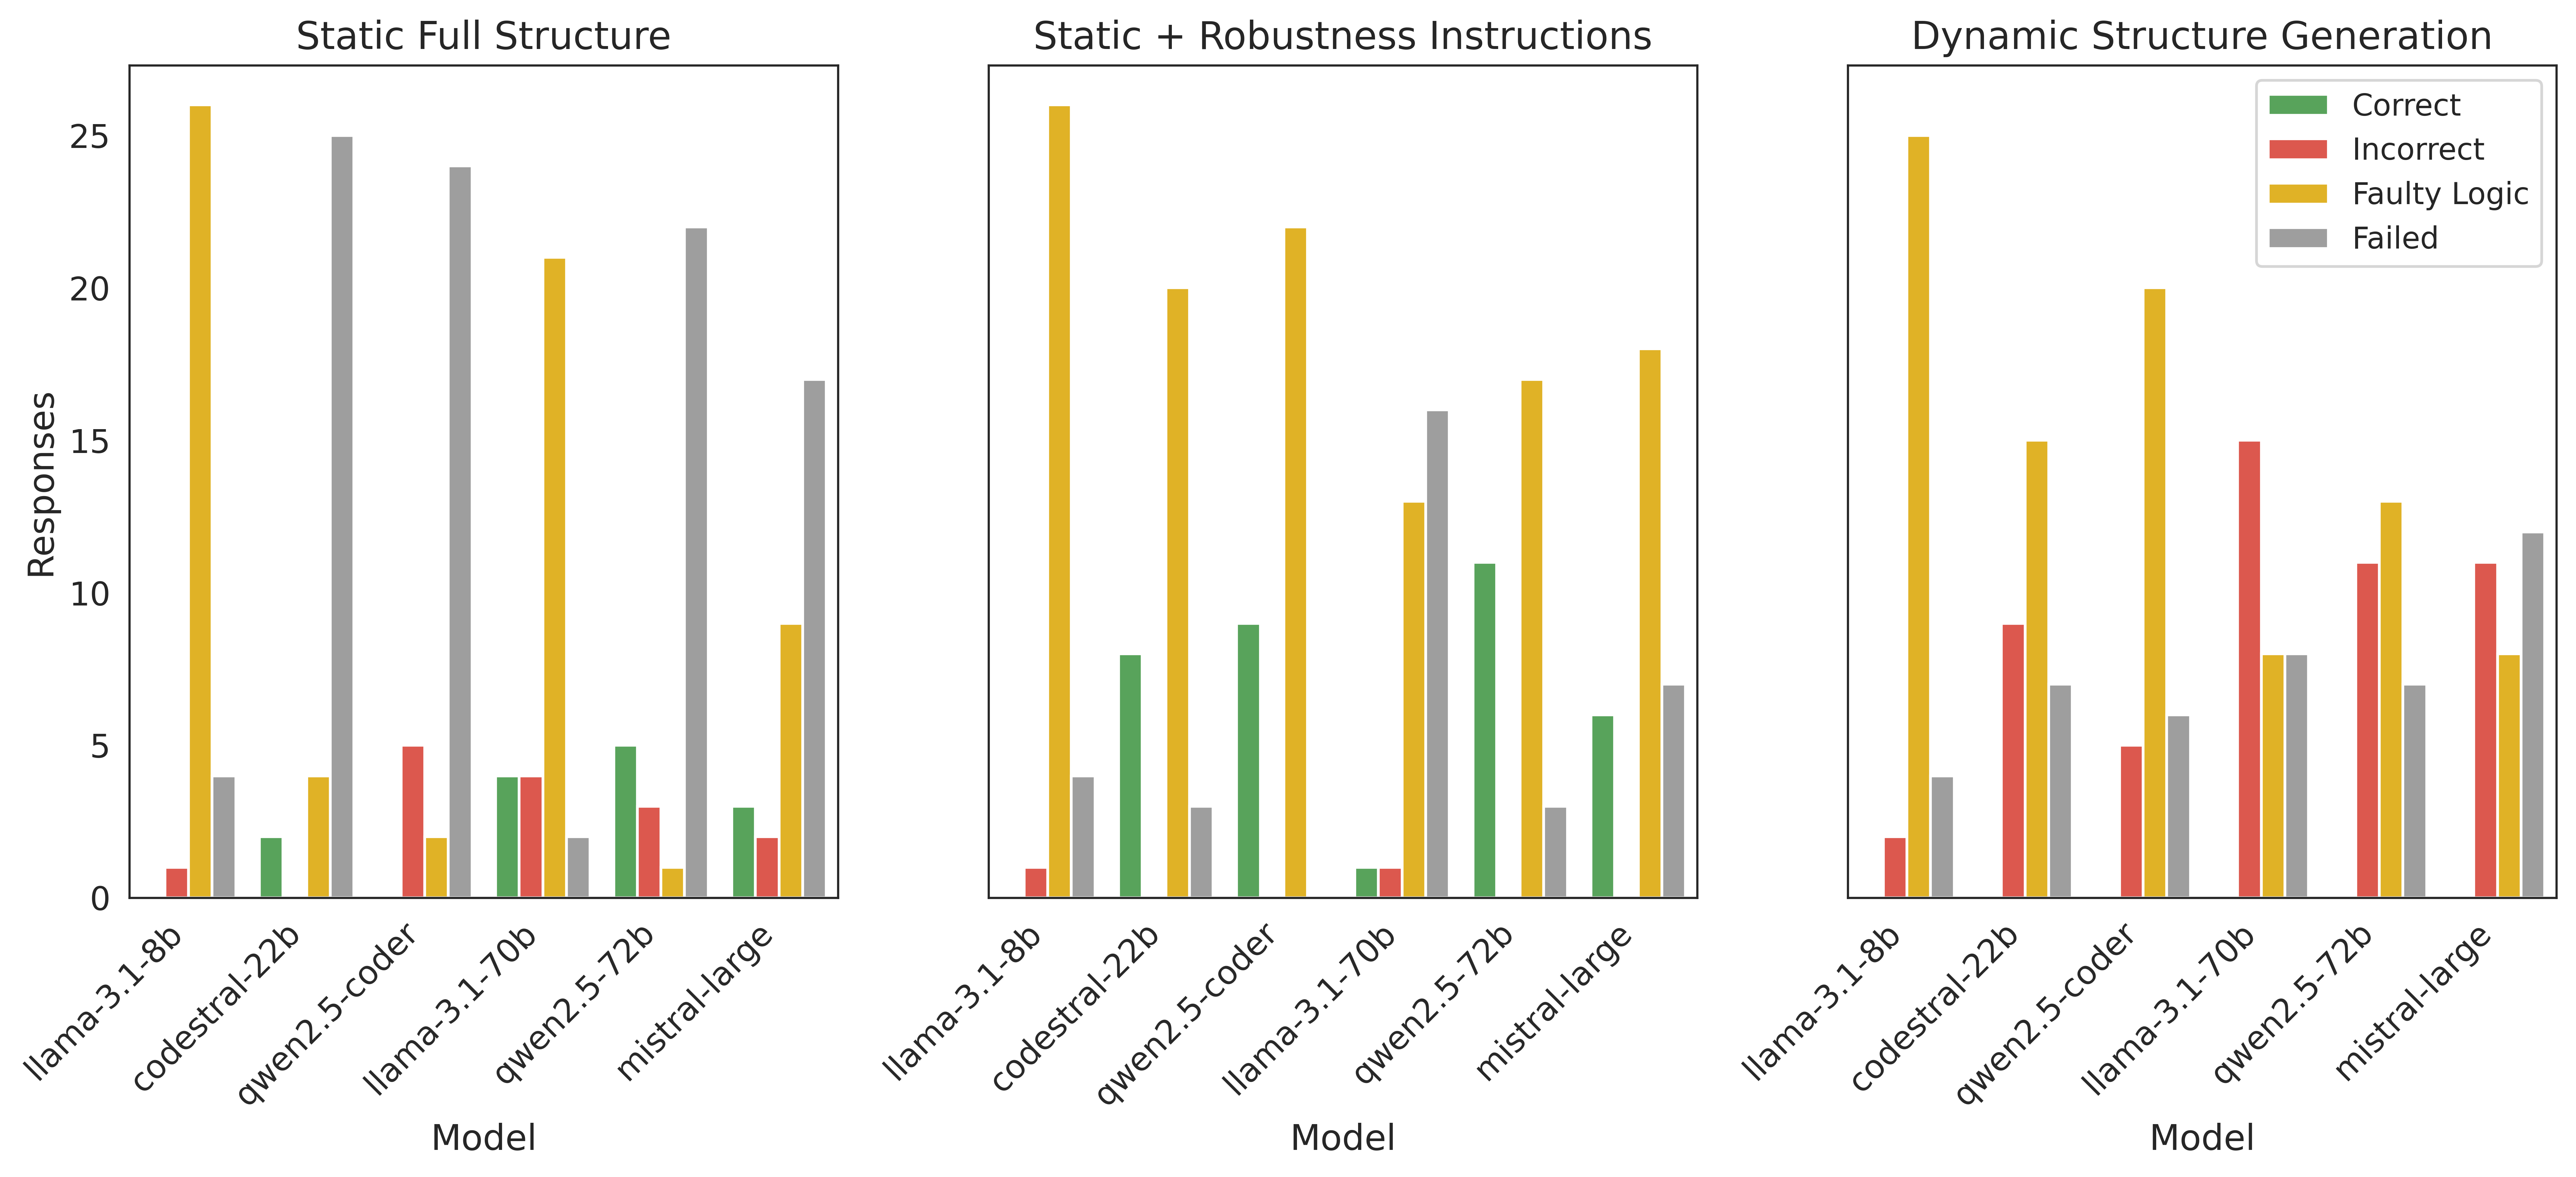
\includegraphics[width=\linewidth]{img/Results/First Experimental Phase/Response Outcome Distribution per Model - No Data.png}
    \caption[Response outcome distribution per model when no relevant data is present]{\textbf{Response outcome distribution per model when no relevant data is present}. Each subplot corresponds to a separate experiment, showing the count of model responses grouped by their evaluation outcome.}
    \label{fig:outcome_distribution_nodata}
\end{figure}

As showcased in Figure~\ref{fig:outcome_distribution_nodata}, when faced with DDPs that lack sufficient information to answer the given question, the second experiment that incorporates robustness instructions performs the best with an accuracy of 18.8\% and a 17.7\% failure rate, which is the lowest among the first-phase experiments. However, 62.4\% of its outputs are still inaccurate due to faulty logic, the highest rate among the experiments. This means that nearly two-thirds of the generated code always produces empty response files, even in datasets that contain sufficient data. In contrast, the dynamic structure generation setup yields the weakest performance, with no correct responses and the highest inaccuracy rate at 28.5\%. In addition, faulty logic is found in 47.8\% of its responses. The static structure experiment ranks in between with accurate responses in only 7.5\% of the instances and has the highest failure rate at 50.5\%, which explains its comparatively lower inaccuracy rate. 

From a model focused perspective (see Figure \ref{fig:outcome_distribution_nodata}), \emph{Llama3.1 8B Instruct} (llama-3.1-8b) performs the worst, producing no correct responses and having the highest share of faulty logic outputs at more than 80\% on all experiments. This explains why it also has one of the lowest failure rates among the models. The most accurate model is \emph{Qwen2.5 72B Instruct} (qwen2.5-72b), achieving 16.1\% accuracy in the first experiment and 35.5\% in the second, the highest among all models in each one. However, it displays high tendencies to produce faulty logic in the second and third experiments. Overall, the remaining models perform similarly poorly, indicating that in this first phase, neither the experimental setups, model size, nor coding-focused training were sufficient to handle missing data scenarios to a desirable extent.

\begin{figure}[ht]
    \centering
    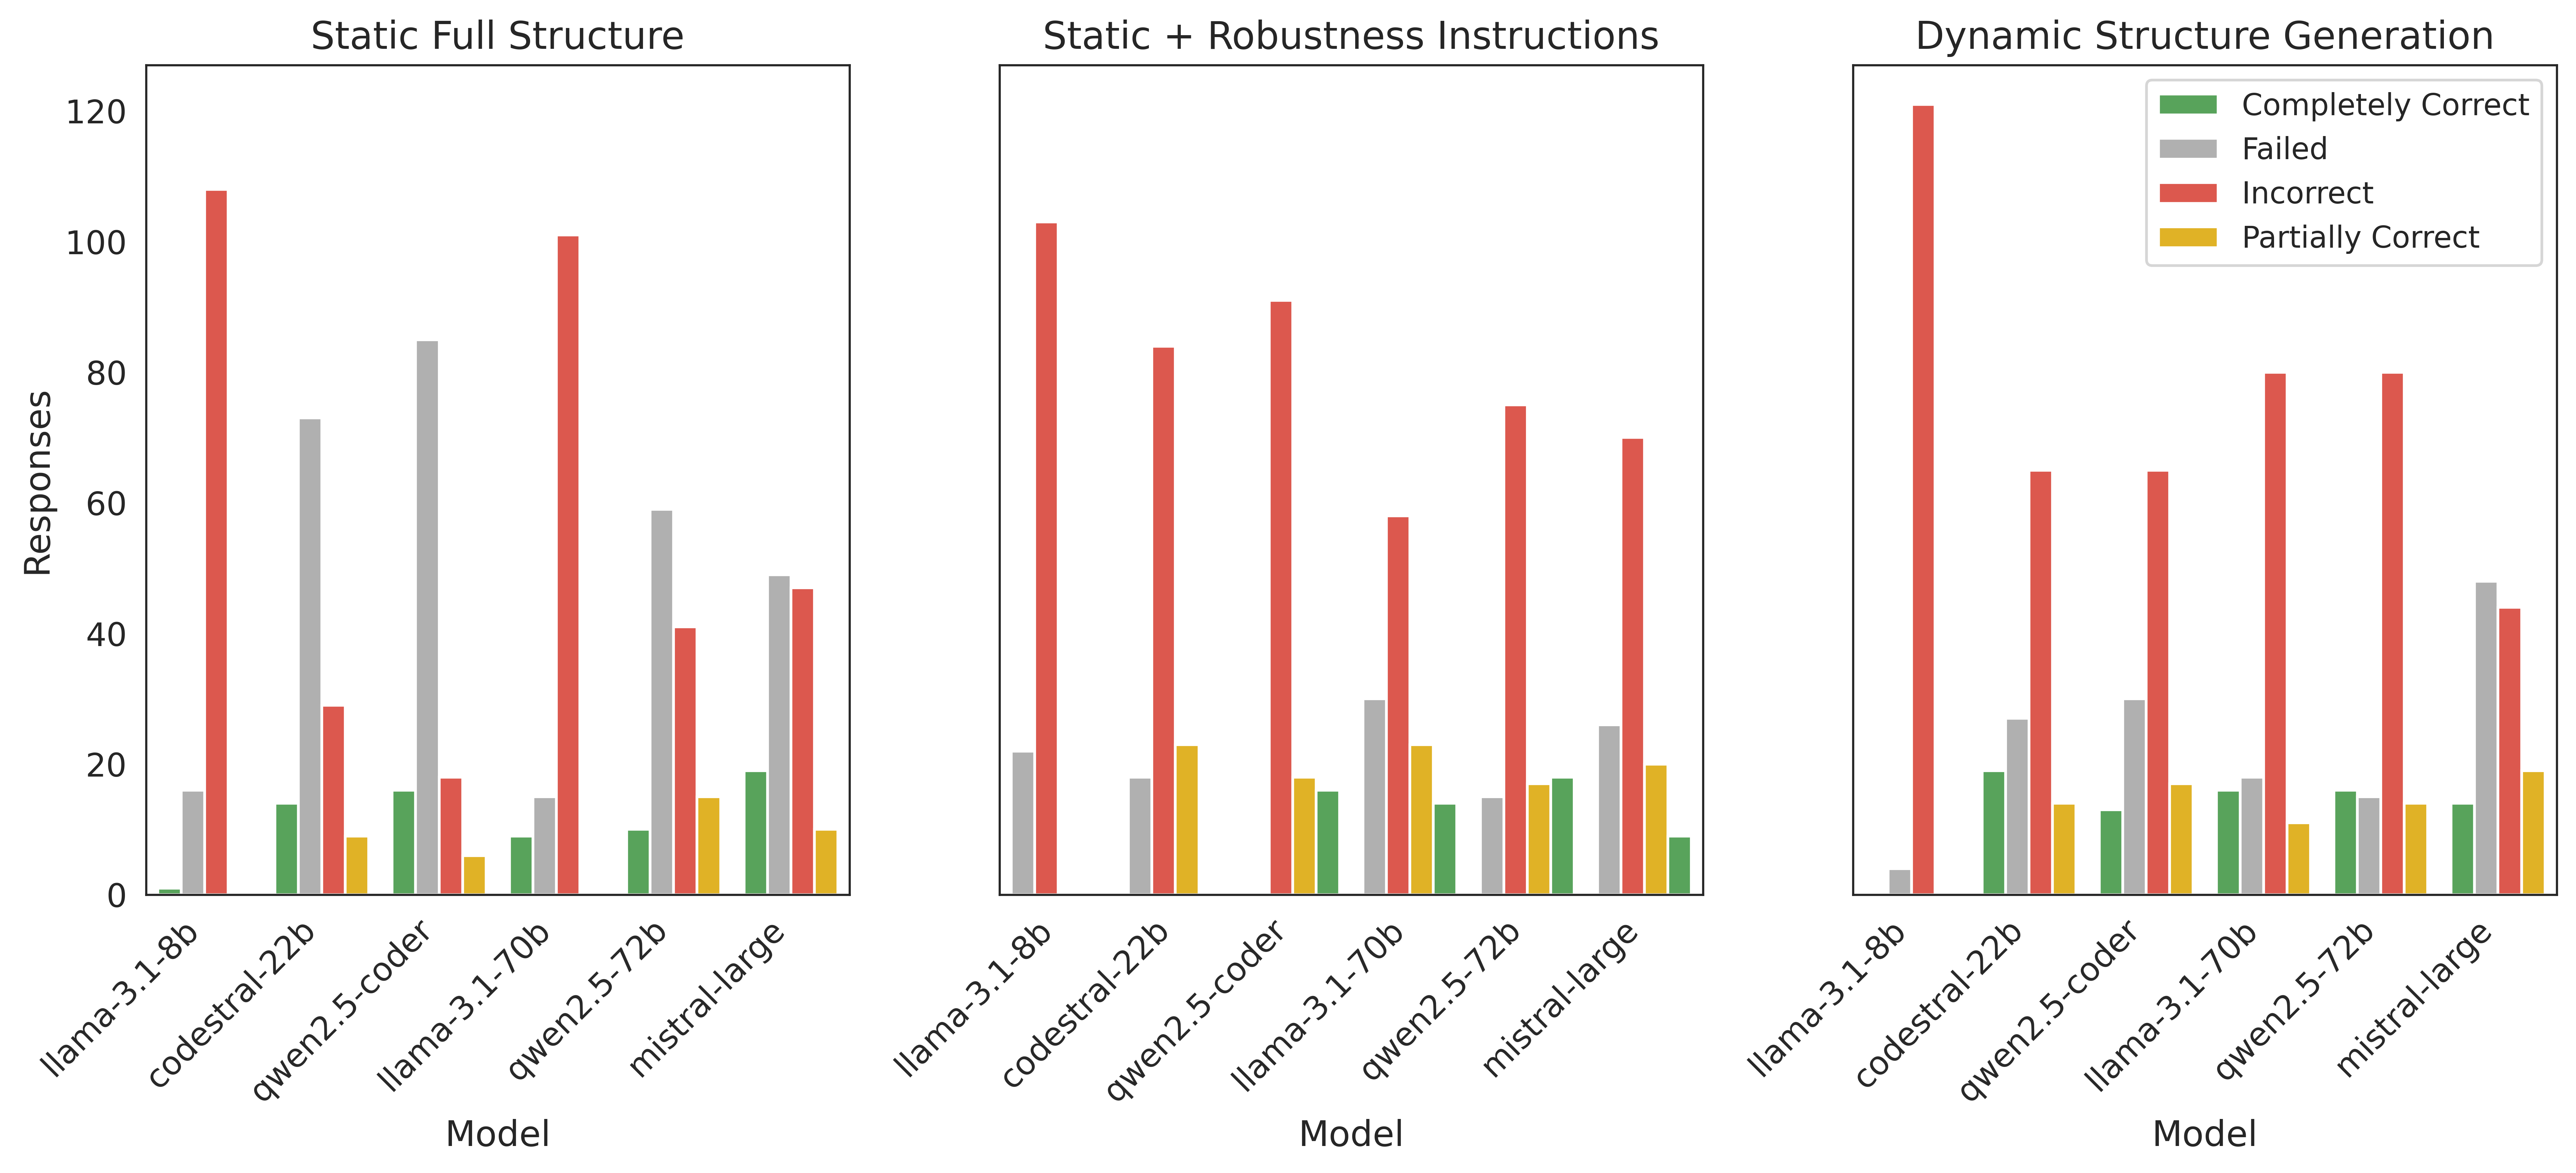
\includegraphics[width=\linewidth]{img/Results/First Experimental Phase/Response Outcome Distribution per Model - With Data.png}
    \caption[Response outcome distribution per model when relevant data is present]{\textbf{Response outcome distribution per model when relevant data is present}. Each subplot corresponds to a separate experiment, showing the count of model responses grouped by their F1 evaluation outcome.}
    \label{fig:outcome_distribution_data}
\end{figure}

When executed on DDPs containing the necessary data, the third experiment achieves the highest proportion of completely correct responses (i.e., responses with an F1 score of 1), at 10.4\%, with a failure rate of 18.9\%. The first experiment follows in accuracy with 9.2\% accurate answers and records the lowest inaccuracy rate, 45.9\%. However, it also exhibits the highest failure rate, 39.6\%, which is expected given the absence of prompt instructions informing the models that some DDPs may lack complete data. The second experiment, which includes robustness instructions, reduces the overall failure rate to 14.8\%, the lowest across all setups, but displays the highest inaccuracy rate, 64.1\%. Although the dynamic structure setup from the third experiment yields the best accuracy, its inaccuracy rate of 60.7\% indicates that relying on models to judge whether the available data is sufficient leads to only modest gains in correctness.

The smallest model in the selection, llama-3.1-8b, achieves some of the lowest failure rates in each experiment, but performs worst in accuracy, with 0.8\% completely correct responses only in the first experiment (see Figure~\ref{fig:outcome_distribution_data}). It has the highest inaccuracy rates, and in the third experiment, this rate goes up to 96.8\%. By contrast, \emph{Codestral 22B Instruct} (codestral-22b) is the most accurate model with a 15.2\% complete accuracy rate in the third experiment. Under the robustness instructions, however, the model doesn't produce any correct responses but instead has the highest rate for partially correct responses at 18.4\%.

For larger models, \emph{Mistral Large Instruct} (mistral-large) achieves the highest rate for completely correct responses at 15.2\% in the first experiment, while qwen2.5-72b leads in the second one at 14.4\%. \emph{Llama3.1 70B Instruct} (llama-3.1-70b) generally performs on par with qwen2.5-72b in terms of complete accuracy, but falls slightly behind in the second experiment.

Overall, all models show a high tendency to produce inaccurate or failing output more than completely or partially accurate ones. These results suggest that different models exhibit distinct accuracy trade-off patterns, with some models avoiding failures but at the cost of accuracy. It can also be highlighted that a larger model size does not necessarily guarantee a better performance, despite the smallest model being essentially the most ineffective for this task. Overall, the RAG-incorporated setup yields very poor performance across the three implemented experiments.

\begin{figure}[ht]
    \centering
    \includegraphics[width=\linewidth]{img/Results/First Experimental Phase/Evaluation of Model Performance Across Experiments.png}
    \caption[Model performance across non-failed experimental instances]{\textbf{Model performance across non-failed experimental instances}. Each subplot represents a distinct experiment, illustrating model performance variations with respect to precision, recall, and F1 score.}
    \label{fig:model_performance_nonfailed}
\end{figure}

\paragraph{Precision, Recall, and F1 Score Performance}\mbox{}\\

\noindent On non-failed experimental instances, the smaller llama-3.1-8b model consistently scores near zero across all metrics, reflecting its limited capability for this task. In contrast, the larger llama-3.1-70b demonstrates improved recall and precision in the second and third experiments but still
trails behind some of the better-performing models. \emph{Qwen2.5 Coder 32B Instruct} (qwen2.5-coder) excels in precision and especially F1 score under the static full structure setup, indicating a moderate ability to generate accurate output. However, its recall is lower than its precision in this setup, suggesting that the model misses some relevant records when responding.

As observed in Figure~\ref{fig:model_performance_nonfailed}, all experiments commonly show average metric values around or below 40\%. Comparing the three experimental settings, the first setup tends to yield higher precision and F1 scores for most models despite having the highest failure rates. The introduction of robustness instructions in the second setup significantly reduces the failure rate. Still, it negatively impacts these metrics, indicating that the high failure rate in the first experiment might be masking the poor model performance observed in the second one. Additionally, for the second and third experiments, most models exhibit higher recall than precision or F1, suggesting that while the models capture most relevant data, they also include many false positives. This behavior lowers the overall balance and hints at the models' tendency to overestimate when answering questions.

\begin{table}[!b]
    \centering
    \renewcommand{\arraystretch}{1.2}
    \setlength{\tabcolsep}{10pt}
    \begin{tabular}{lccc}
        \hline
        \textbf{Model} & 
        \makecell{\textbf{Static Full} \\ \textbf{Structure}} & 
        \makecell{\textbf{Static + Robustness} \\ \textbf{Instructions}} & 
        \makecell{\textbf{Dynamic Structure} \\ \textbf{Generation}} \\
        \hline
        llama-3.1-8b   & \cellcolor{red!15} $0.01 \pm 0.10$ & \cellcolor{red!15} $0.00 \pm 0.00$ & \cellcolor{red!15} $0.00 \pm 0.00$ \\
        codestral-22b   & $0.32 \pm 0.44$ & $0.06 \pm 0.14$ & $0.28 \pm 0.43$ \\
        qwen2.5-coder   & $0.40 \pm 0.49$ & $0.23 \pm 0.39$ & $0.27 \pm 0.42$ \\
        llama-3.1-70b   & $0.08 \pm 0.28$ & $0.33 \pm 0.43$ & $0.20 \pm 0.38$ \\
        qwen2.5-72b     & $0.28 \pm 0.41$ & $0.26 \pm 0.41$ & $0.22 \pm 0.39$ \\
        mistral-large   & $0.36 \pm 0.47$ & $0.23 \pm 0.38$ & $0.34 \pm 0.44$ \\
        \hline
    \end{tabular}
    \caption[Model F1 score performance and consistency]{\textbf{Model F1 score performance and consistency}. This table provides an overview of the mean F1 scores and standard deviations for each model under the three experimental conditions.}
    \label{tab:F1_and_st_deviation}
\end{table}

When analyzing the models' accuracy further in Table~\ref{tab:F1_and_st_deviation}, we observe that, except for llama-3.1-8b, which performs the worst, all the other models across the experiments exhibit a standard deviation higher than their mean F1 score. While some degree of stochasticity is expected from LLMs, considering that this setup involves asking the models the same questions across the selected DDPs, we highlight notable inconsistency and fluctuation in their performance. This indicates that the setup introduces considerable instability, making it risky to entirely rely on these models for this task without further performance improvements.

\paragraph{Model Answering Behavior}\mbox{}\\

\noindent Considering the methodology framework regarding how models generate structured responses (refer to Subsection~\ref{performance_metrics}), alongside completely correct responses, we can distinguish between several partially correct and incorrect answer types across the experiments when investigating non-failed experimental instances (see Figure~\ref{fig:answer_type_classification}). 

\begin{figure}[ht]
    \centering
    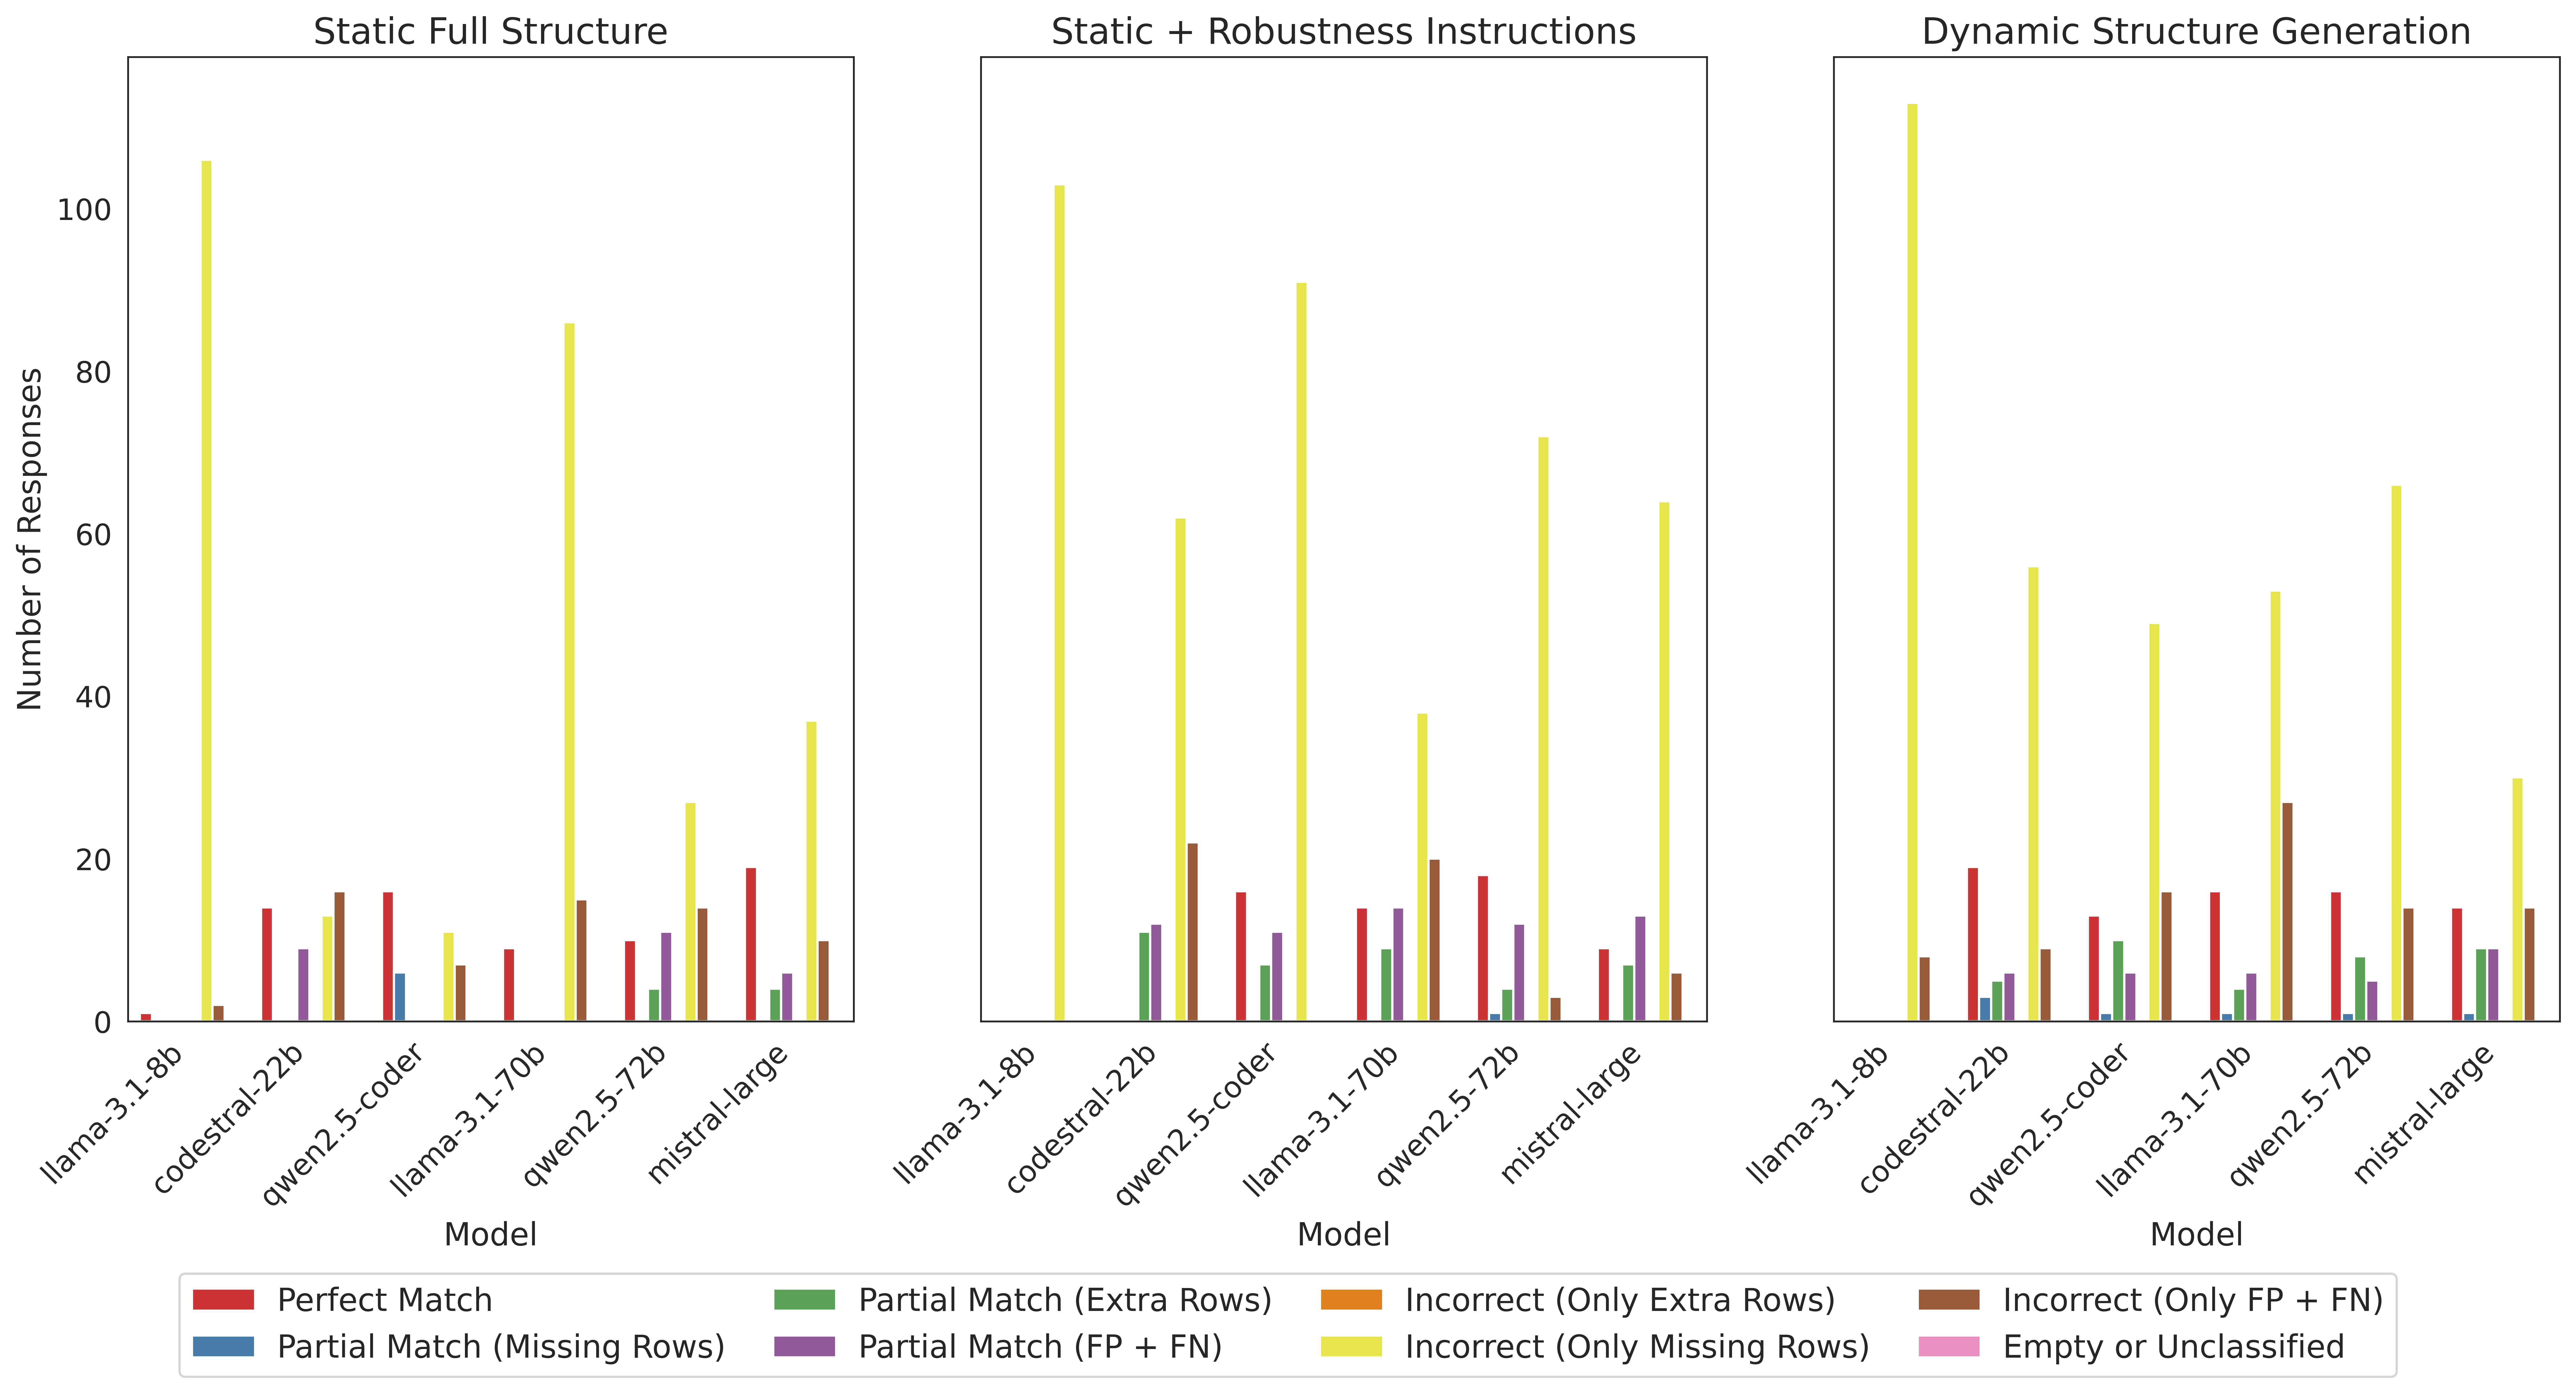
\includegraphics[width=\linewidth]{img/Results/First Experimental Phase/Answer Type Classification per Model Across Experiments.png}
    \caption[Distribution of answer types by model and experimental setup]{\textbf{Distribution of answer types by model and experimental setup}. Each subplot represents a distinct experiment, illustrating the distribution of response types for each model. Responses are categorized into Perfect Matches, Partial Matches (with subtypes for missing or extra rows), and Incorrect outcomes (with subtypes for extra, missing, or both types of inaccurate rows).}
    \label{fig:answer_type_classification}
\end{figure}

Upon examining the models' answering trends, we find that across all experiments, the most common answer type involves only missing rows. In the first and third experiments, at least 14.1\% of responses contain only FP and FN, indicating that the models selected incorrect files to extract data from. The second experiment stands out for producing more partially correct responses than entirely correct ones. Notably, in both the first and second experiments, partial matches that involve FP and FN are the dominant type of partially correct responses. In these cases, the models extract an accurate subset of the data but also include unnecessary records. Under the dynamic structure setup, partially correct answers are more likely to include extra rows when compared to other setups.

From a model-specific perspective, llama-3.1-8b produces empty files in 96.7\% of its responses, with the other models ranging from 50–58\% as well. Only qwen2.5-coder and llama-3.1-70b seem to produce more completely correct than partially correct responses, but only at 17.3\% and 12.5\% respectively. In all other cases, models generate more FP + FN in partially correct outputs, and even more FP + FN in incorrect outputs, reinforcing the observation that the models often focus on the wrong files when mapping questions to the data structure.

\paragraph{Question-wise Model Comparative Analysis}\mbox{}\\

\begin{figure}[!b]
    \centering
    \includegraphics[width=\linewidth]{img/Results/First Experimental Phase/F1 Score Heatmaps (Model × Question).png}
    \caption[F1 score heatmaps by model and question across experiments]{\textbf{F1 score heatmaps by model and question across experiments}. Each heatmap represents a distinct experiment, illustrating the model performance per question. Higher scores (darker shades of red) indicate better model accuracy for that question-experiment pair.}
    \label{fig:f1_score_heatmap}
\end{figure}

\noindent Figure~\ref{fig:f1_score_heatmap} illustrates which questions the models struggle with the least across the three experiments. Notably, questions 2 and 3, as well as the last three questions, are consistently easier to answer, a trend observed in all experiments. This is interesting because the later questions are generally designed to be more complex, involving calculations and operations across multiple files. This suggests that the models' performance is not directly correlated with any of the questions' difficulty.

As discussed earlier, the static structure experiment shows the highest failure rate, but here the codestral-22b and qwen2.5-coder models demonstrate notably high accuracy on some of the questions they answer, albeit only on two questions each. The robustness experiment improves the failure rate and accuracy on some questions compared to the static setup. However, it also lowers accuracy for others. The dynamic structure experiment yields intriguing results. Here, the models are able to answer more questions, but at the cost of overall accuracy. Across most questions, the models achieve moderate performance, while the mid-tier questions (5-8) remain the most challenging.

Contrary to initial expectations, no single model or experiment consistently outperforms others across all questions. Instead, Figure~\ref{fig:f1_score_heatmap} indicates that certain models excel in answering questions related to specific domains within Instagram's data, such as user activity and topic summaries. Questions about account changes or interaction patterns are more challenging for the models, possibly due to them involving time-sensitive data or requiring the synthesis of records over multiple events. While the better performance can be extended to other question domains, the accuracy is likely to drop.

\paragraph{Retries and Their Impact on Performance}\mbox{}\\

\noindent If a model fails to generate executable code on its first attempt, it is allowed up to five retries to overcome the runtime failure and produce valid code. The models in the first experiment's setup require more retries, reflecting the high failure rate of this experiment. In particular, codestral-22b, qwen2.5-coder, and qwen2.5-72b average at least three to four retries. Both the robustness instructions and the dynamic structure generation reduce the average retries needed for successful execution, with the former yielding the lowest retry attempts across all experiments. However, most models exhibit high volatility and inconsistency in the number of attempts required to generate valid code (see Table~\ref{tab:retry_mean_and_st_deviation}). Consequently, establishing a reliable expected retry range for a model or a given experimental setup remains a difficult task.

\begin{table}[h]
    \centering
    \renewcommand{\arraystretch}{1.2}
    \setlength{\tabcolsep}{10pt}
    \begin{tabular}{lccc}
        \hline
        \textbf{Model} & 
        \makecell{\textbf{Static Full} \\ \textbf{Structure}} & 
        \makecell{\textbf{Static + Robustness} \\ \textbf{Instructions}} & 
        \makecell{\textbf{Dynamic Structure} \\ \textbf{Generation}} \\
        \hline
        llama-3.1-8b & $0.94 \pm 2.03$ & $1.22 \pm 2.23$ & $0.54 \pm 1.45$ \\
        codestral-22b & $3.80 \pm 2.89$ & $0.82 \pm 2.05$ & $1.26 \pm 2.44$ \\
        qwen2.5-coder & $4.12 \pm 2.79$ & $0.00 \pm 0.00$ & $1.37 \pm 2.51$ \\
        llama-3.1-70b & $0.99 \pm 1.99$ & $1.74 \pm 2.62$ & $1.17 \pm 2.22$ \\
        qwen2.5-72b & $3.16 \pm 2.96$ & $0.72 \pm 1.93$ & $1.13 \pm 2.15$ \\
        mistral-large & $2.55 \pm 2.93$ & $1.61 \pm 2.51$ & $2.24 \pm 2.90$ \\
        \hline
    \end{tabular}
    \caption[Summary of model retries across experiments]{\textbf{Summary of model retries across experiments}. The average number of execution attempts and the standard deviation for each model across the experimental setups.}
    \label{tab:retry_mean_and_st_deviation}
\end{table}

Analyzing how F1 scores change across these attempts helps in defining a minimum retry threshold, which might potentially reduce the execution or API request scope, or even determine if retries are needed at all in this setup. As shown in Figure~\ref{fig:retries_vs_F1}, most experimental instances are concentrated on the first attempt (no retries), which also contains the largest cluster of high F1 scores, including perfect scores of 1. As the number of attempts increases, experimental instances become increasingly concentrated at an F1 score of 0, with fewer examples in intermediate or high ranges. Notably, some larger models achieve high F1 scores on the second and third attempts. In a unique and separate case, llama-3.1-8b reaches perfect accuracy once on the fourth attempt. By contrast, the fifth attempt yields only inaccurate results, and the final attempt produces only a handful of moderate scores. Since in most cases, the highest accuracies are achieved on the first try, these results suggest retries may not be necessary at all in a RAG-enhanced setup, or could be limited to three attempts to lower computational costs.

\begin{figure}[ht]
    \centering
    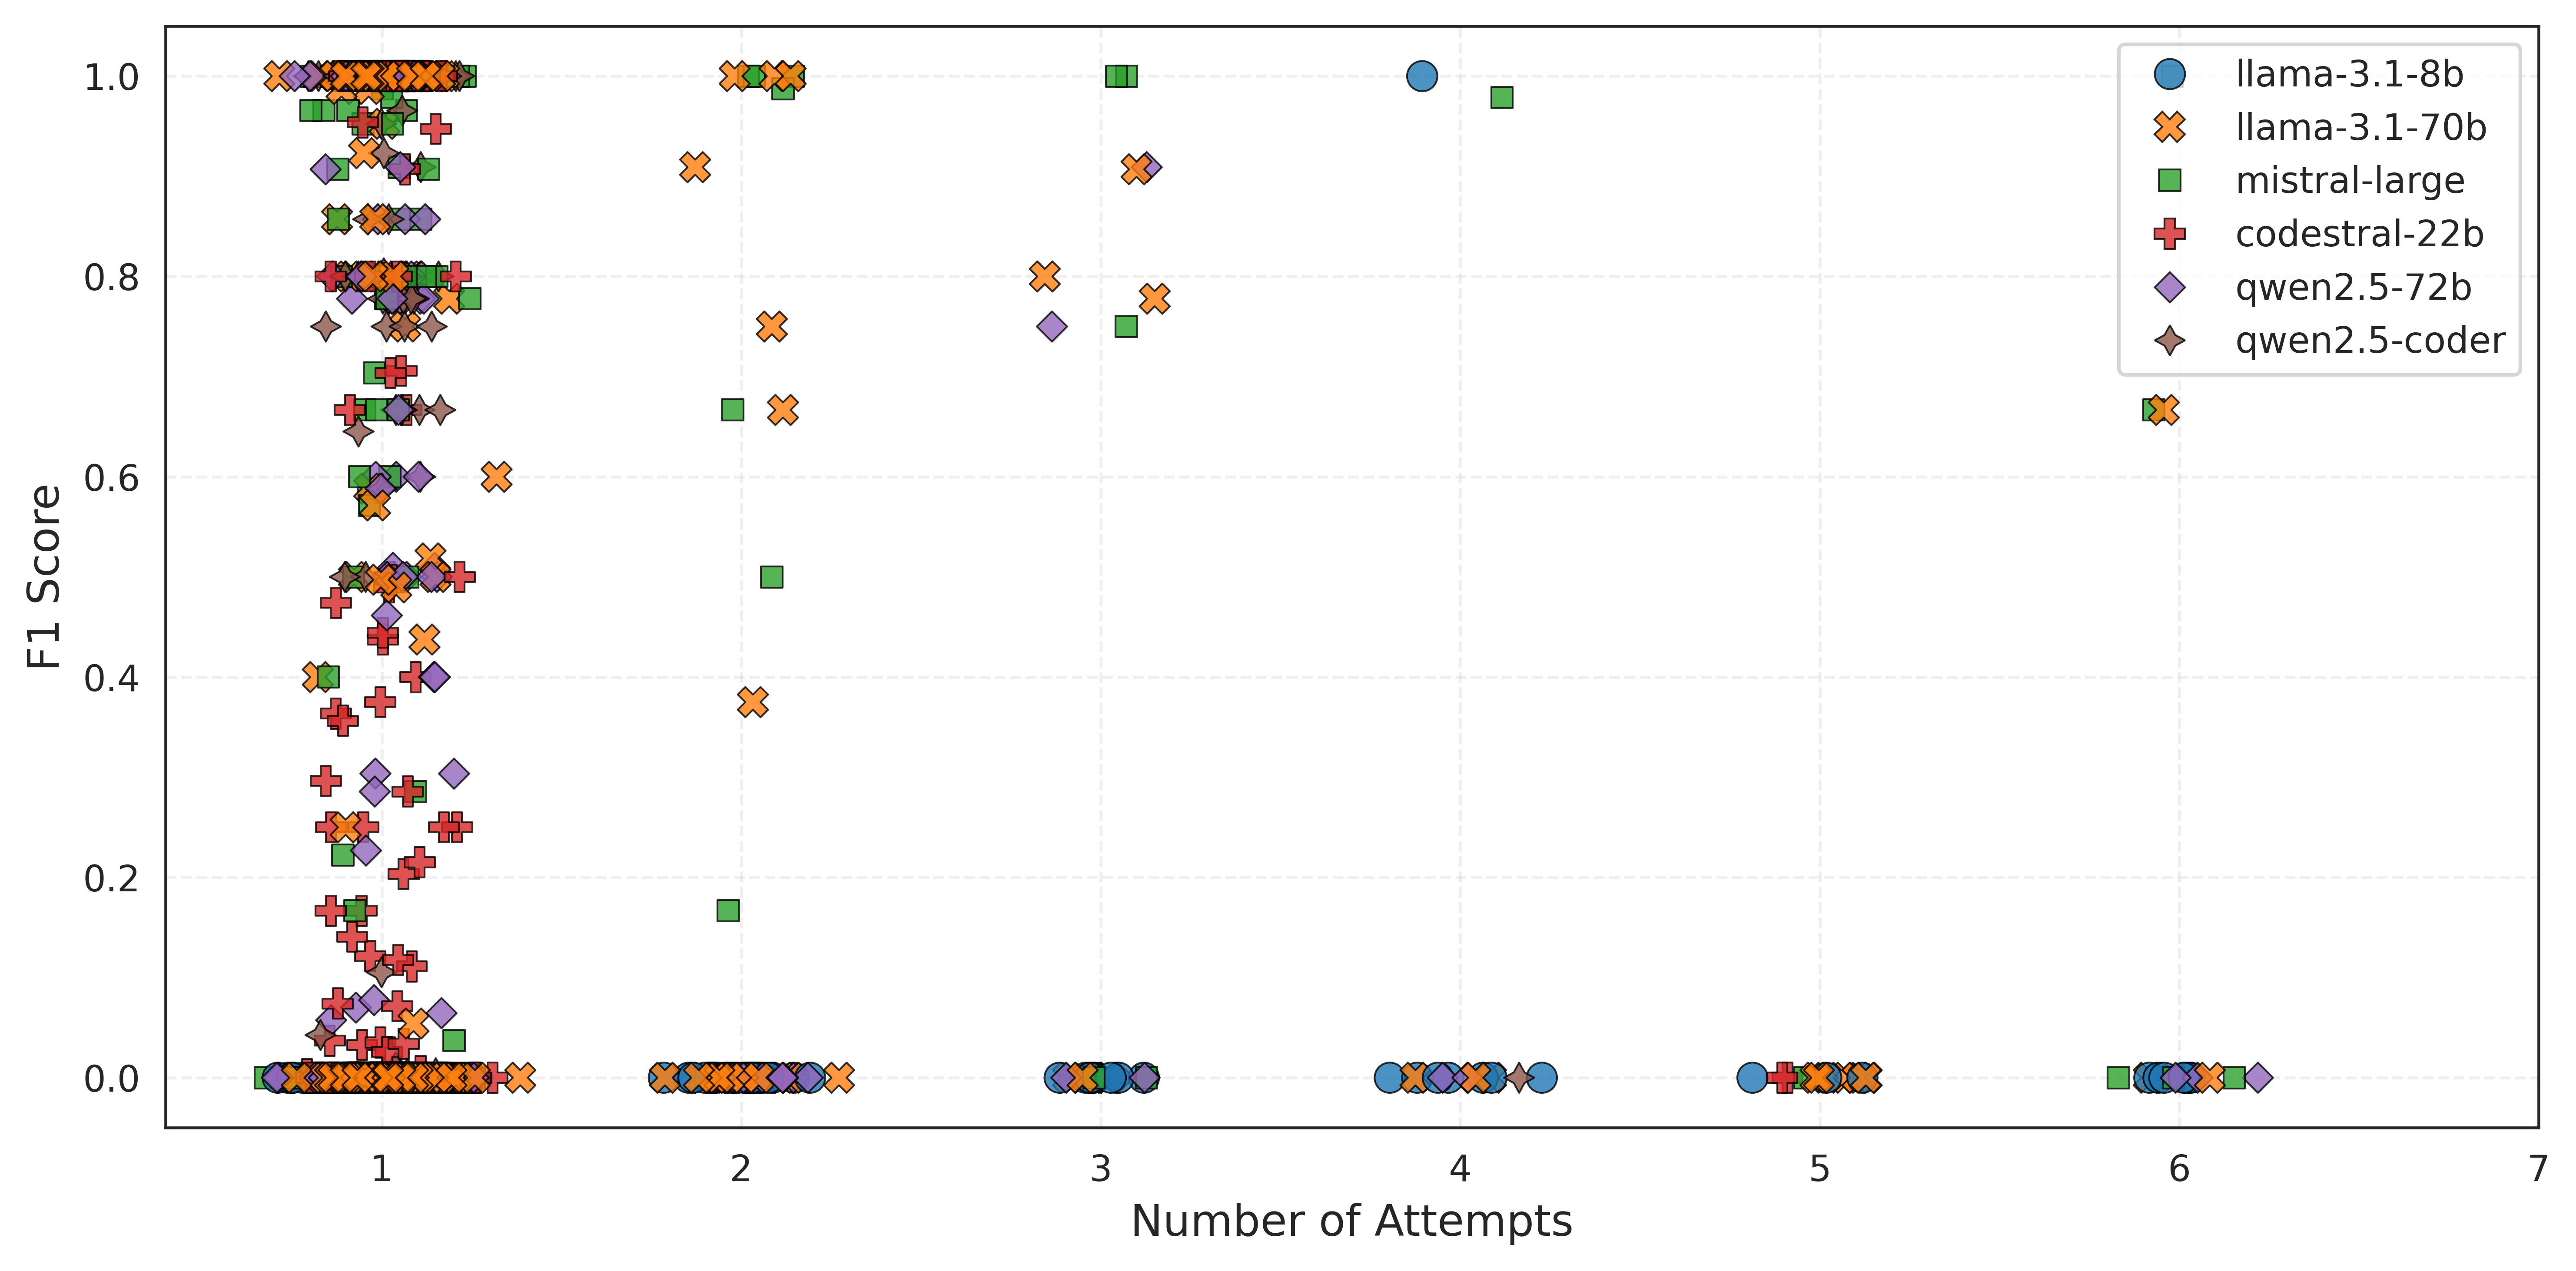
\includegraphics[width=\linewidth]{img/Results/First Experimental Phase/Number of Retries vs F1 Score.png}
    \caption[Number of attempts vs. F1 score across models]{\textbf{Number of attempts vs. F1 score across models}. This scatter plot illustrates the relationship between the number of retries (attempts) and the achieved F1 score for various models evaluated across all experiments. Each point represents an individual experimental instance, with a slight jitter applied to improve visibility. Different colors and markers distinguish the models to facilitate comparison. The x-axis shows the total number of attempts (initial attempt plus retries).}
    \label{fig:retries_vs_F1}
\end{figure}

\subsection{Error Analysis} \label{RAG_error_analysis}

Among the most common runtime errors, due to the nature of the experiment itself, the FileNotFoundError is the most prominent across all models. This is also the error most likely to occur on the very first generation attempt. When examining the generated scripts, models often tend to misphrase or generate incorrect file paths, frequently removing one or two levels of the provided folder hierarchy. If the generated code handles missing files, this can explain the high number of inaccurate responses that contain only FN. 

Other frequent errors, such as KeyError, UnicodeEncodeError, AttributeError, and others, appear to result from invalid script generation and wrongful data processing. All errors shown in Figure~\ref{fig:error_frequency}, along with InvalidTimeStampFormat and IndexError, are considered “persistent” errors. Once these errors occur on the first generation attempt, they typically recur in subsequent retries until the retry limit is reached and the instance ends in failure. In most cases, the models seem unable to mitigate these errors despite multiple retries. For the FileNotFoundError, this is understandable, as the model may be confident in the incorrect file path it generates and does not attempt to fix it. However, the other persistent error types indicate failures in handling data extraction, processing issues, or fundamental flaws in the generated scripts.

\begin{figure}[ht]
    \centering
    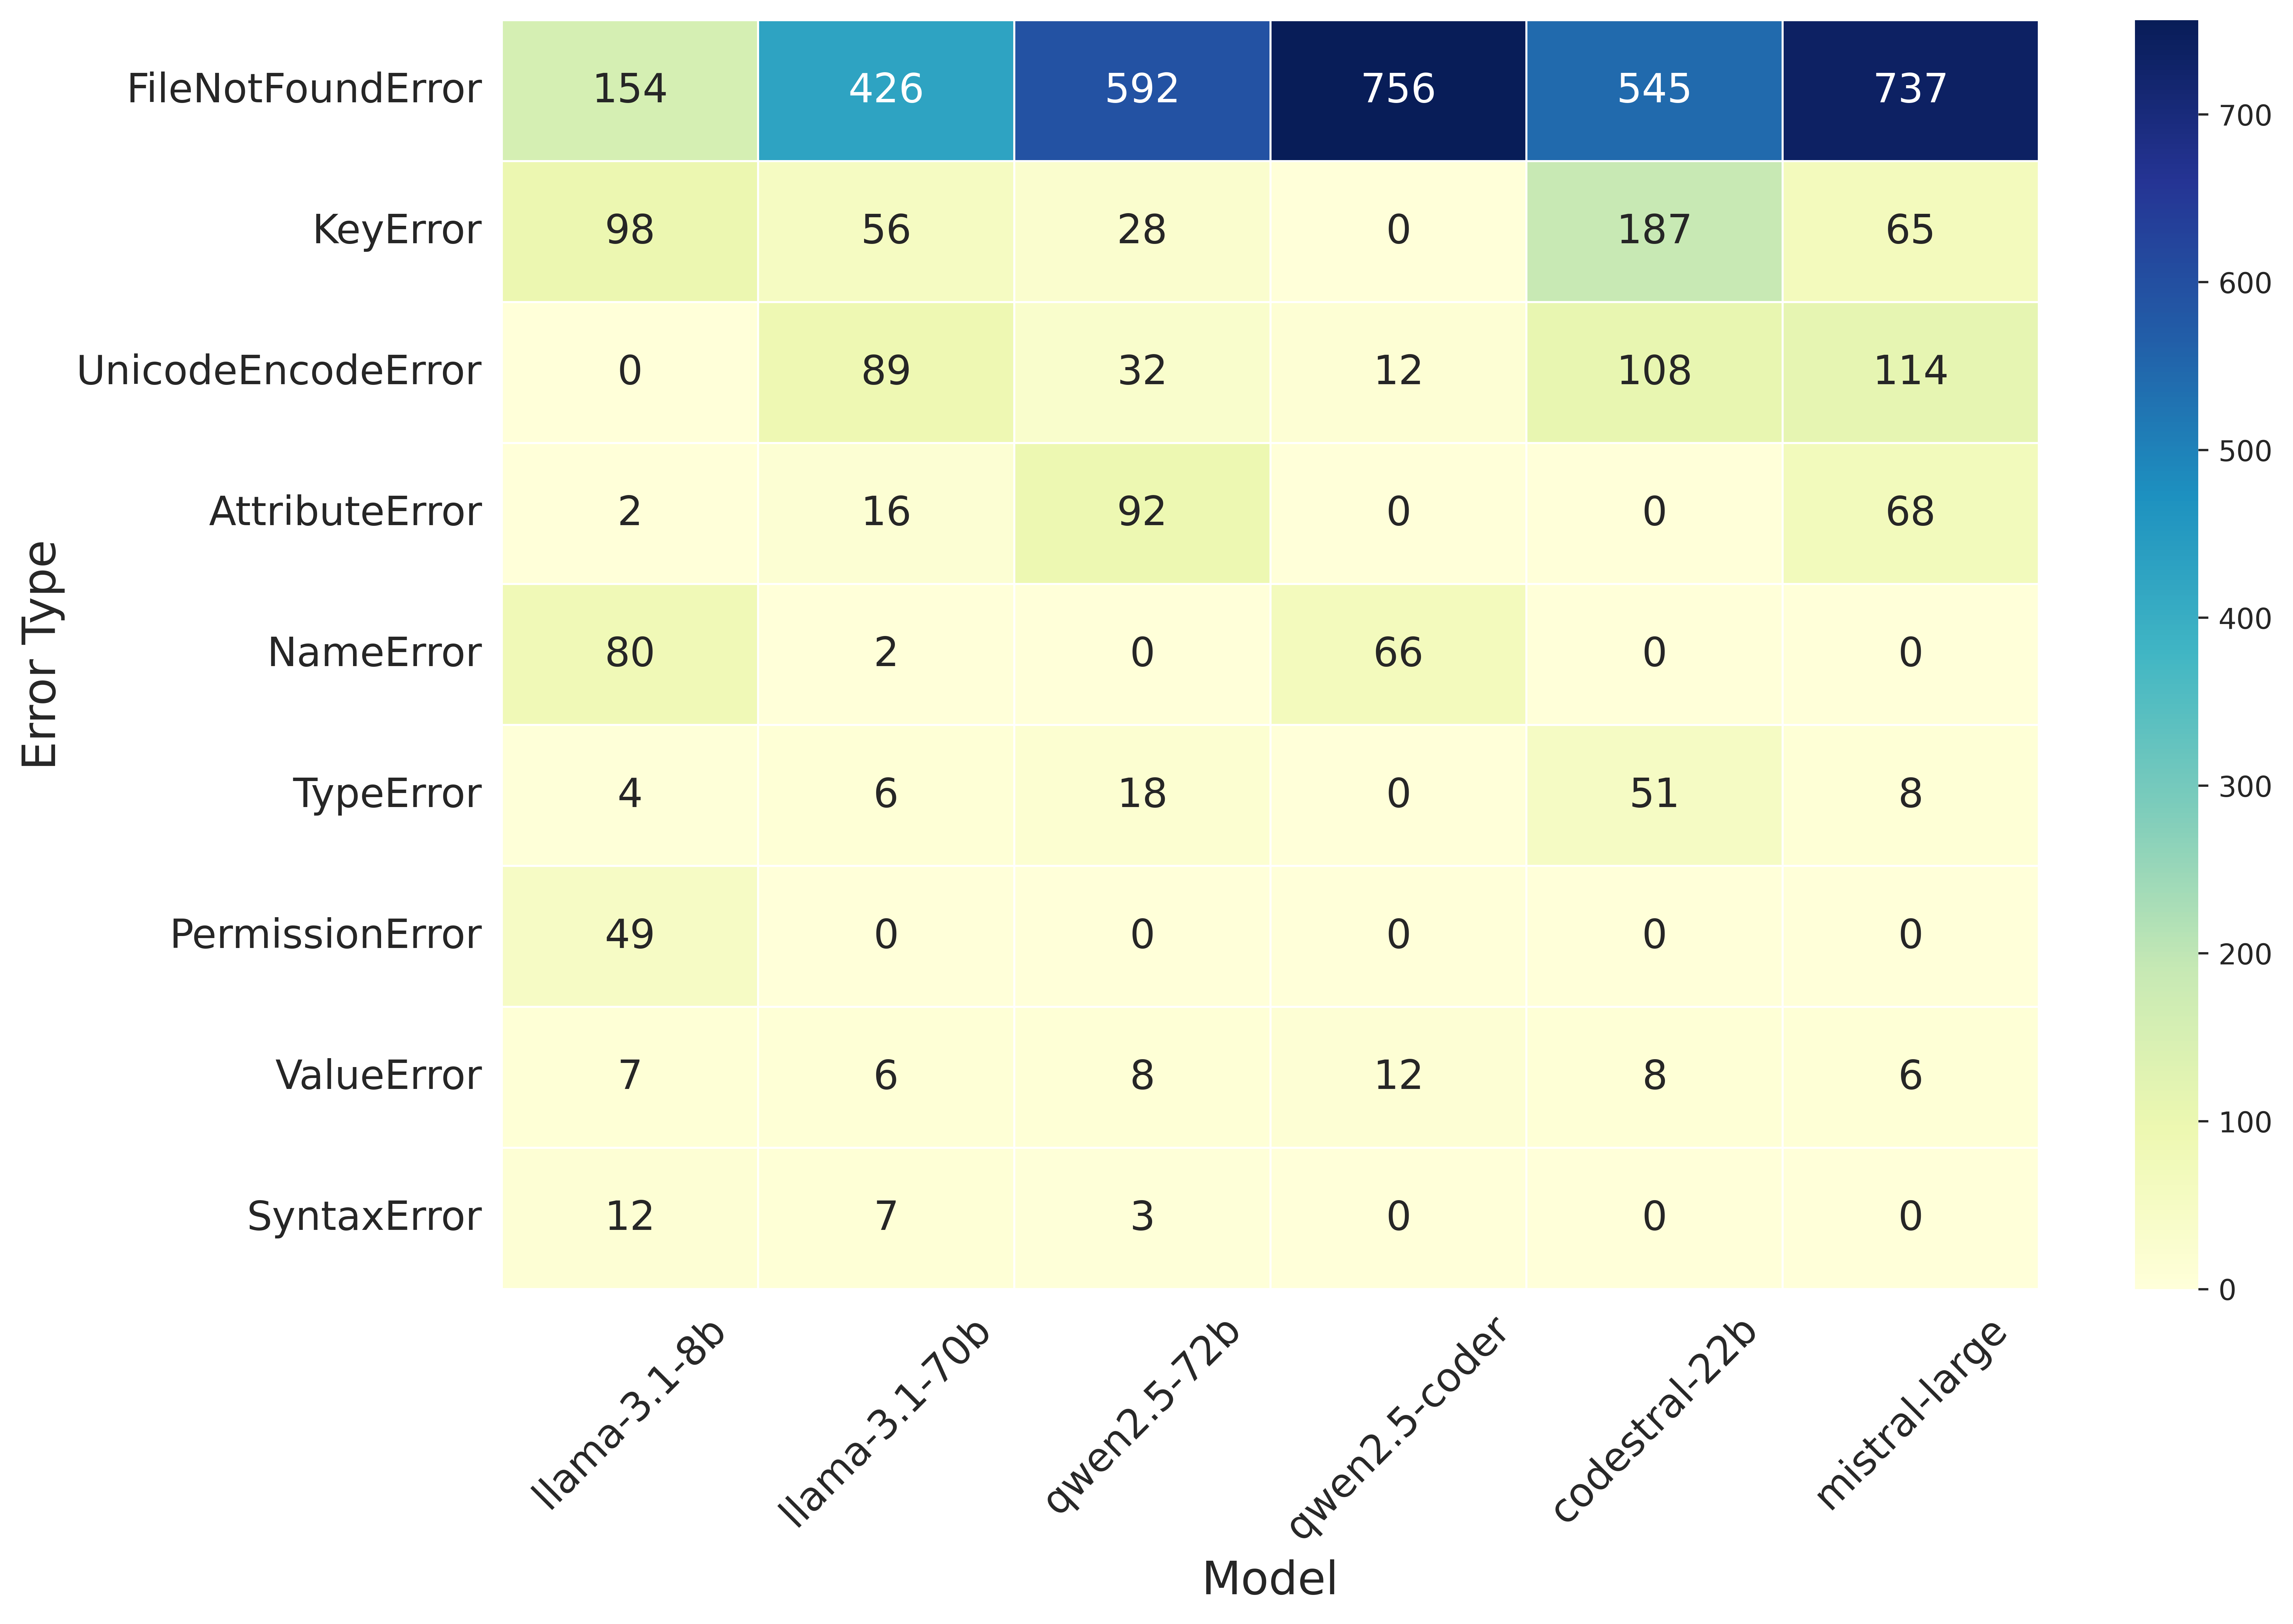
\includegraphics[width=0.80\linewidth]{img/Results/First Experimental Phase/Error Type Frequency per Model.png}
    \caption[Error type frequency per model]{\textbf{Error type frequency per model}. Heatmap showing the frequency of the nine most common error types across all evaluated models, aggregated from all experiments. Each cell represents the number of occurrences for a given error type–model pair, with color intensity indicating frequency. Models are ordered from lowest to highest total error count, and error types are ranked from most to least frequent.}
    \label{fig:error_frequency}
\end{figure}

Among the models, qwen2.5-coder is the one most prone to generating code with FileNotFoundError. Along with codestral-22b, both of which are specifically trained for coding tasks, it ranks among the highest generators of erroneous code in this experimental phase. In contrast, llama-3.1-8b produces the fewest errors, a result of its highly inaccurate but executable code. Meanwhile, the largest model in the selection, mistral-large, is the one most likely to generate errors for this task. An interesting insight from Figure~\ref{fig:error_frequency} is that the models seem to be grouped by their developers based on how likely they are to generate faulty code. Models developed by Meta have the fewest errors, followed by those from Alibaba Cloud. The models most prone to errors are those developed by Mistral.

\begin{figure}[ht]
    \centering
    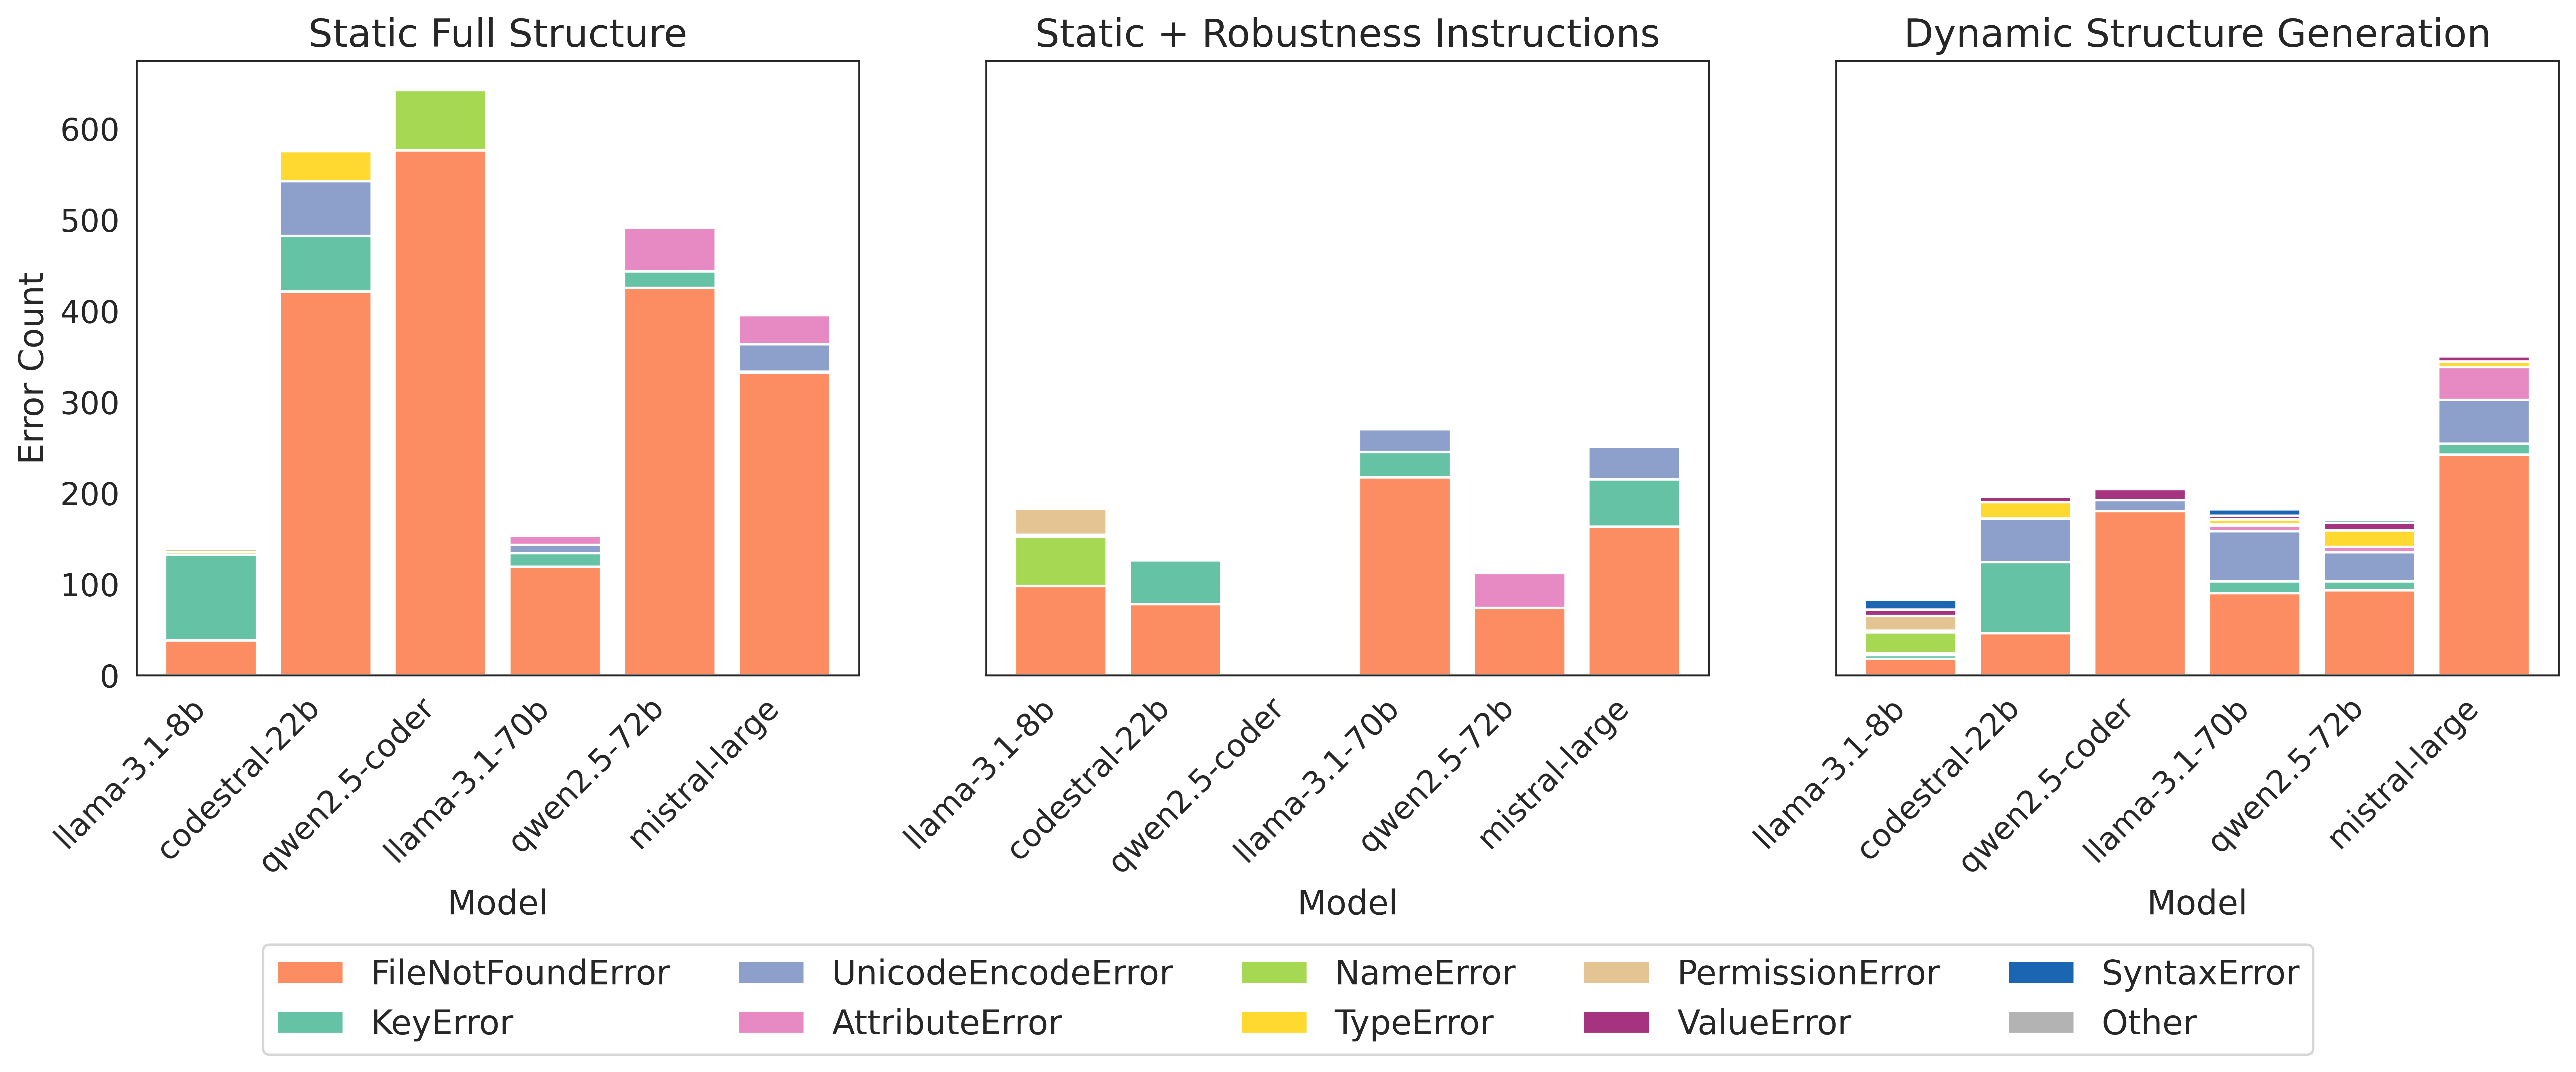
\includegraphics[width=\linewidth]{img/Results/First Experimental Phase/Error Type Distribution per Model.png}
    \caption[Error type distribution]{\textbf{Error type distribution}. The stacked bar charts illustrate the frequency of the nine most common error types encountered for each model, grouped by experiment. Only the top 9 most frequent error types are shown explicitly, while all other less frequent errors are aggregated under “Other”.}
    \label{fig:error_distribution}
\end{figure}

The additional prompt instructions in the second and third experiments significantly reduce the occurrence of FileNotFoundError compared to the first experiment. However, this error remains the most frequent one in this first experimental phase (see Figure~\ref{fig:error_distribution}). The models' tendency to generate incorrect paths appears to persist regardless of the experimental setup or the provided data structure.

Qwen2.5-coder shows impressive improvement under the robustness instructions, producing error-free code in this experiment. A stark contrast to the first experiment, where it is the most error-prone model. However, the dynamic structure generation negatively impacts its performance, leading it to produce erroneous code once again. This new set of errors is not dominated by FileNotFoundError, but instead by KeyError and UnicodeEncodeError. Alongside NameError, these emerge as the next most frequent error types across the experiments, again highlighting the models' faulty processing and extraction techniques. Furthermore, the dynamic generation instructions appear to introduce a greater variety in the types of errors present in the models' outputs.

\begin{figure}[ht]
    \centering
    
\includegraphics[width=\linewidth]{img/Results/First Experimental Phase/Error Trend Over Attempts.png}
    \caption[Error frequency trends over successive attempts]{\textbf{Error frequency trends over successive attempts}. The trend of error counts across multiple attempt numbers for each model, separated by experimental setup.}
    \label{fig:error_trends}
\end{figure}

Figure~\ref{fig:error_trends} illustrates the models' ability to reduce runtime errors through retries. In the static structure experiment, only the Llama models show moderate improvement in eliminating these errors from their generated code. In contrast, qwen2.5-coder struggles the most among the models, failing to mitigate erroneous behavior in its code across all attempts. The remaining models display slight improvements after their first attempt, but any error not resolved by the second attempt tends to persist until failure.

This pattern extends to the second and third experiments as well. In the former, mistral-large, and in the latter, qwen2.5-72B, alongside the Llama models, are the only ones to reduce errors through retries successfully. The other models in their respective setups fail to do so. The presence of persistent error types appears to have significantly hindered these models' attempts to correct their previous coding mistakes. Overall, the Llama models are the most consistent performers across all experiments, demonstrating an aptitude to successfully eliminate errors from their code, whether to a slight or moderate extent.

\subsection{Generated Code Analysis}

The selected code evaluation metrics are primarily employed to compare the successfully executable generated scripts across models and to provide an estimate of their expected performance within the scope of data analysis tasks.

\paragraph{Raw and Halstead Metrics}\mbox{}\\

\noindent Code documentation and explanatory comments may improve understandability, but are not directly linked to better performance. Since providing comments in code is a subjective practice, we examine each model's documentation habits (see Figure~\ref{fig:comment_density_and_halstead}).

\begin{figure}[!b]
    \centering
    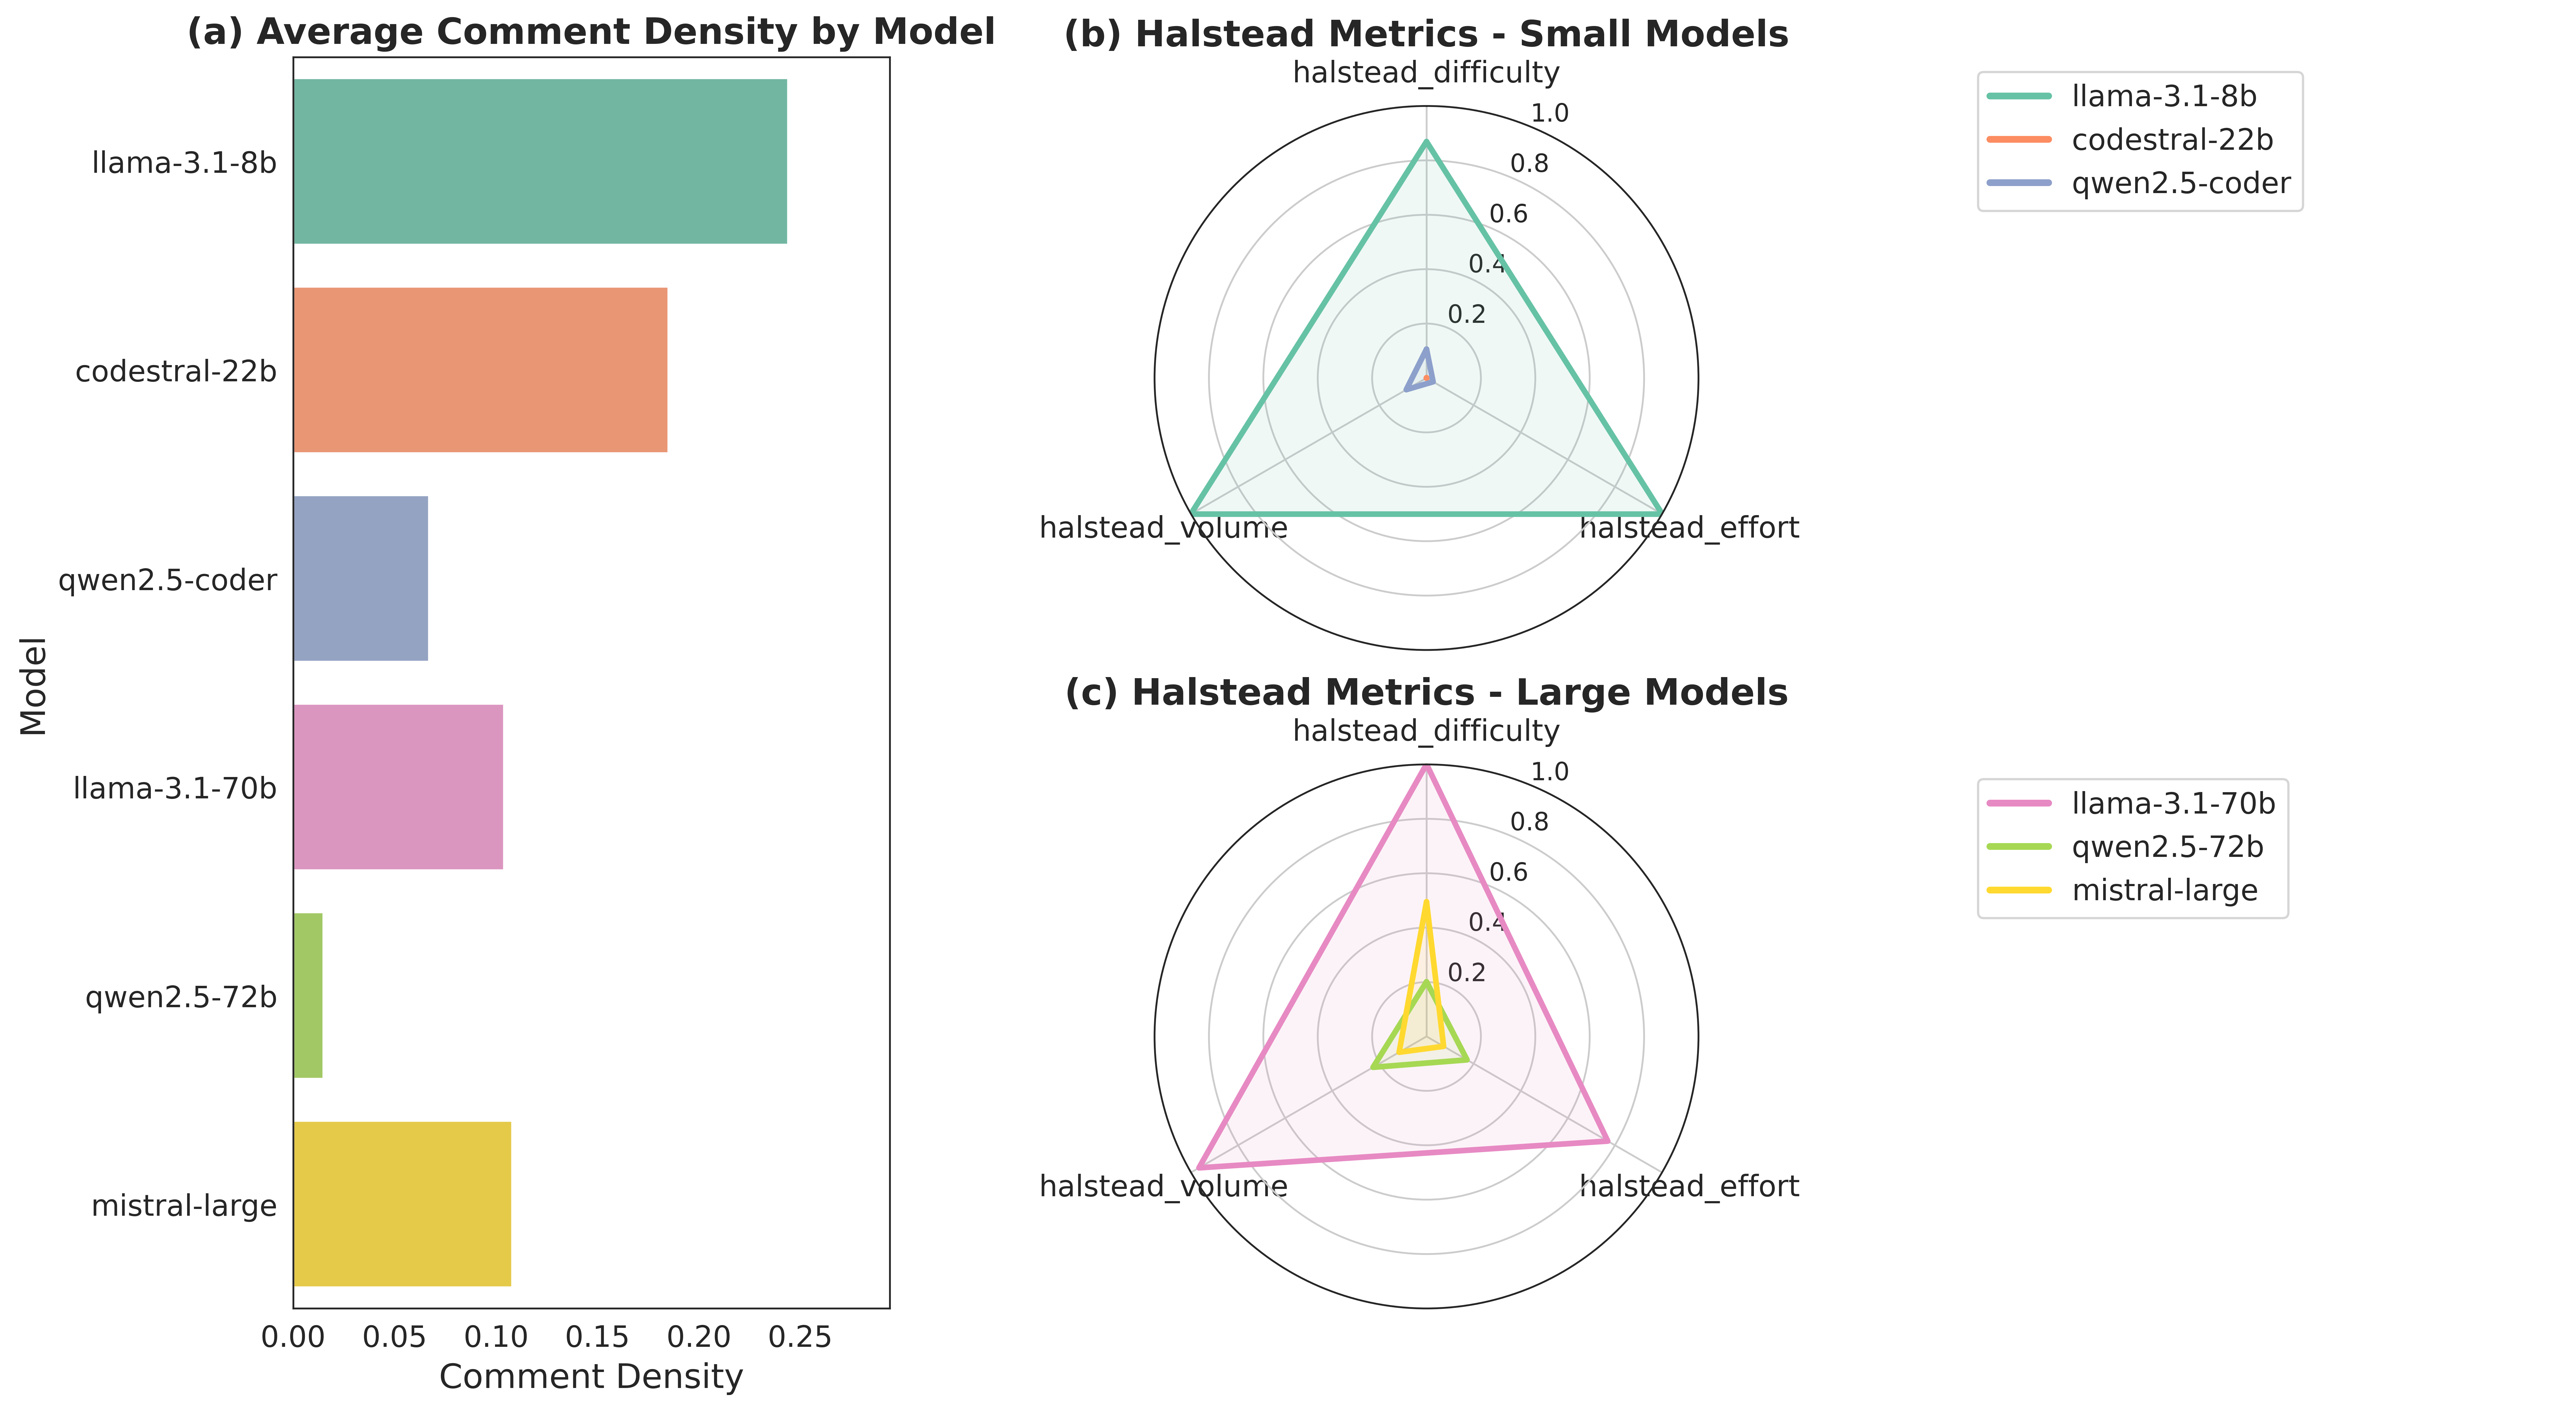
\includegraphics[width=\linewidth]{img/Results/First Experimental Phase/Comment_Density_and_Halstead_Radar.png}
    \caption[Comment density and Halstead metrics across models]{\textbf{Comment density and Halstead metrics across models}. The bar plot (a) shows the average proportion of comments in generated code by each model. The radar charts present normalized Halstead metrics for small (b) and large (c) models, grouped by their size.}
    \label{fig:comment_density_and_halstead}
\end{figure}

The most inaccurate model, llama-3.1-8b, has the highest average comment density, with 24.4\% of its output consisting of comments. This means that this model generates roughly one comment for every four lines of code, a strong tendency to document compared to the other models. The second smallest model, codestral-22b, follows with a density of 18.5\%. At the opposite end, qwen2.5-coder and qwen2.5-72b produce the fewest comments, at about 6.7\% and 1.5\% respectively, with the latter averaging only one comment per around 67 lines of code. These models, developed by Alibaba Cloud, may be optimized for concise, production-style commenting rather than lengthy documentation. Overall, excluding qwen2.5-coder, the larger models tend to produce fewer comments than the smaller ones. 


When examining the Halstead metrics for the small models (see Figure~\ref{fig:comment_density_and_halstead}), llama-3.1-8b records the highest difficulty, effort, and volume values. This suggests that its generated code is structurally more complex, thereby increasing the cognitive load required for understanding and maintenance. This complexity aligns with the model's previously observed tendency toward extensive inline documentation, indicating that both contribute to a more elaborate output style. In contrast, codestral-22b yields the lowest values across all three Halstead dimensions, implying that its generated code is minimalistic and structurally simple compared to the rest. Similarly, qwen2.5-coder also produces relatively low complexity code, reflecting these two models' code specialized training that may favor streamlined solutions over intricate implementations. The larger counterpart, qwen2.5-72b, likewise exhibits comparatively low complexity and effort, which appears consistent with the Qwen models' generally sparse documentation habits.

A similar pattern is observed for the large models, where llama-3.1-70b achieves the highest Halstead metrics in its group. Across both size categories, the Llama models generate the most complex code according to Halstead measures. Models with very low Halstead values, such as codestral-22b and qwen2.5-coder, tend to favor simpler, more direct solutions.

\paragraph{Cyclomatic Complexity}\mbox{}\\

\noindent To further examine the characteristics of the selected models' code generation habits, Figure~\ref{fig:cyc_loc_correlation} presents the relationship between LOC and total cyclomatic complexity across all experiments.

\begin{figure}[ht]
    \centering
    \includegraphics[width=\linewidth]{img/Results/First Experimental Phase/Cyc_LOC_correlation.png}
    \caption[]{\textbf{Relationship between lines of code and cyclomatic complexity}. Scatter plots illustrating the relationship between source code size and total cyclomatic complexity for small and large models across the experiments. Regression lines (dashed) highlight overall trends, while $R^2$ values indicate the proportion of variance in cyclomatic complexity explained by LOC.}
    \label{fig:cyc_loc_correlation}
\end{figure}

The smaller models exhibit a strong positive relationship with coefficients of determination $R^2\approx55$ in both the static and dynamic structure experiments. This suggests that, for smaller models, increases in code length tend to correspond to proportional increases in structural complexity, indicating somewhat predictable scaling of code intricacy. In contrast, larger models generally show weaker correlations between LOC and complexity across experiments, with only the third experiment coming closest at an $R^2$ of 0.40. This lower correlation may reflect that larger models generate more varied code structures whose complexity does not scale as consistently with length.

Between the two model size categories, several outliers with comparatively high cyclomatic complexity relative to code size come from the Llama models. This pattern indicates that these models sometimes produce code that is structurally more complex for the given LOC compared to the other models, which might reflect either more sophisticated logic or potentially unnecessary code complexity. 

\begin{figure}[ht]
    \centering
    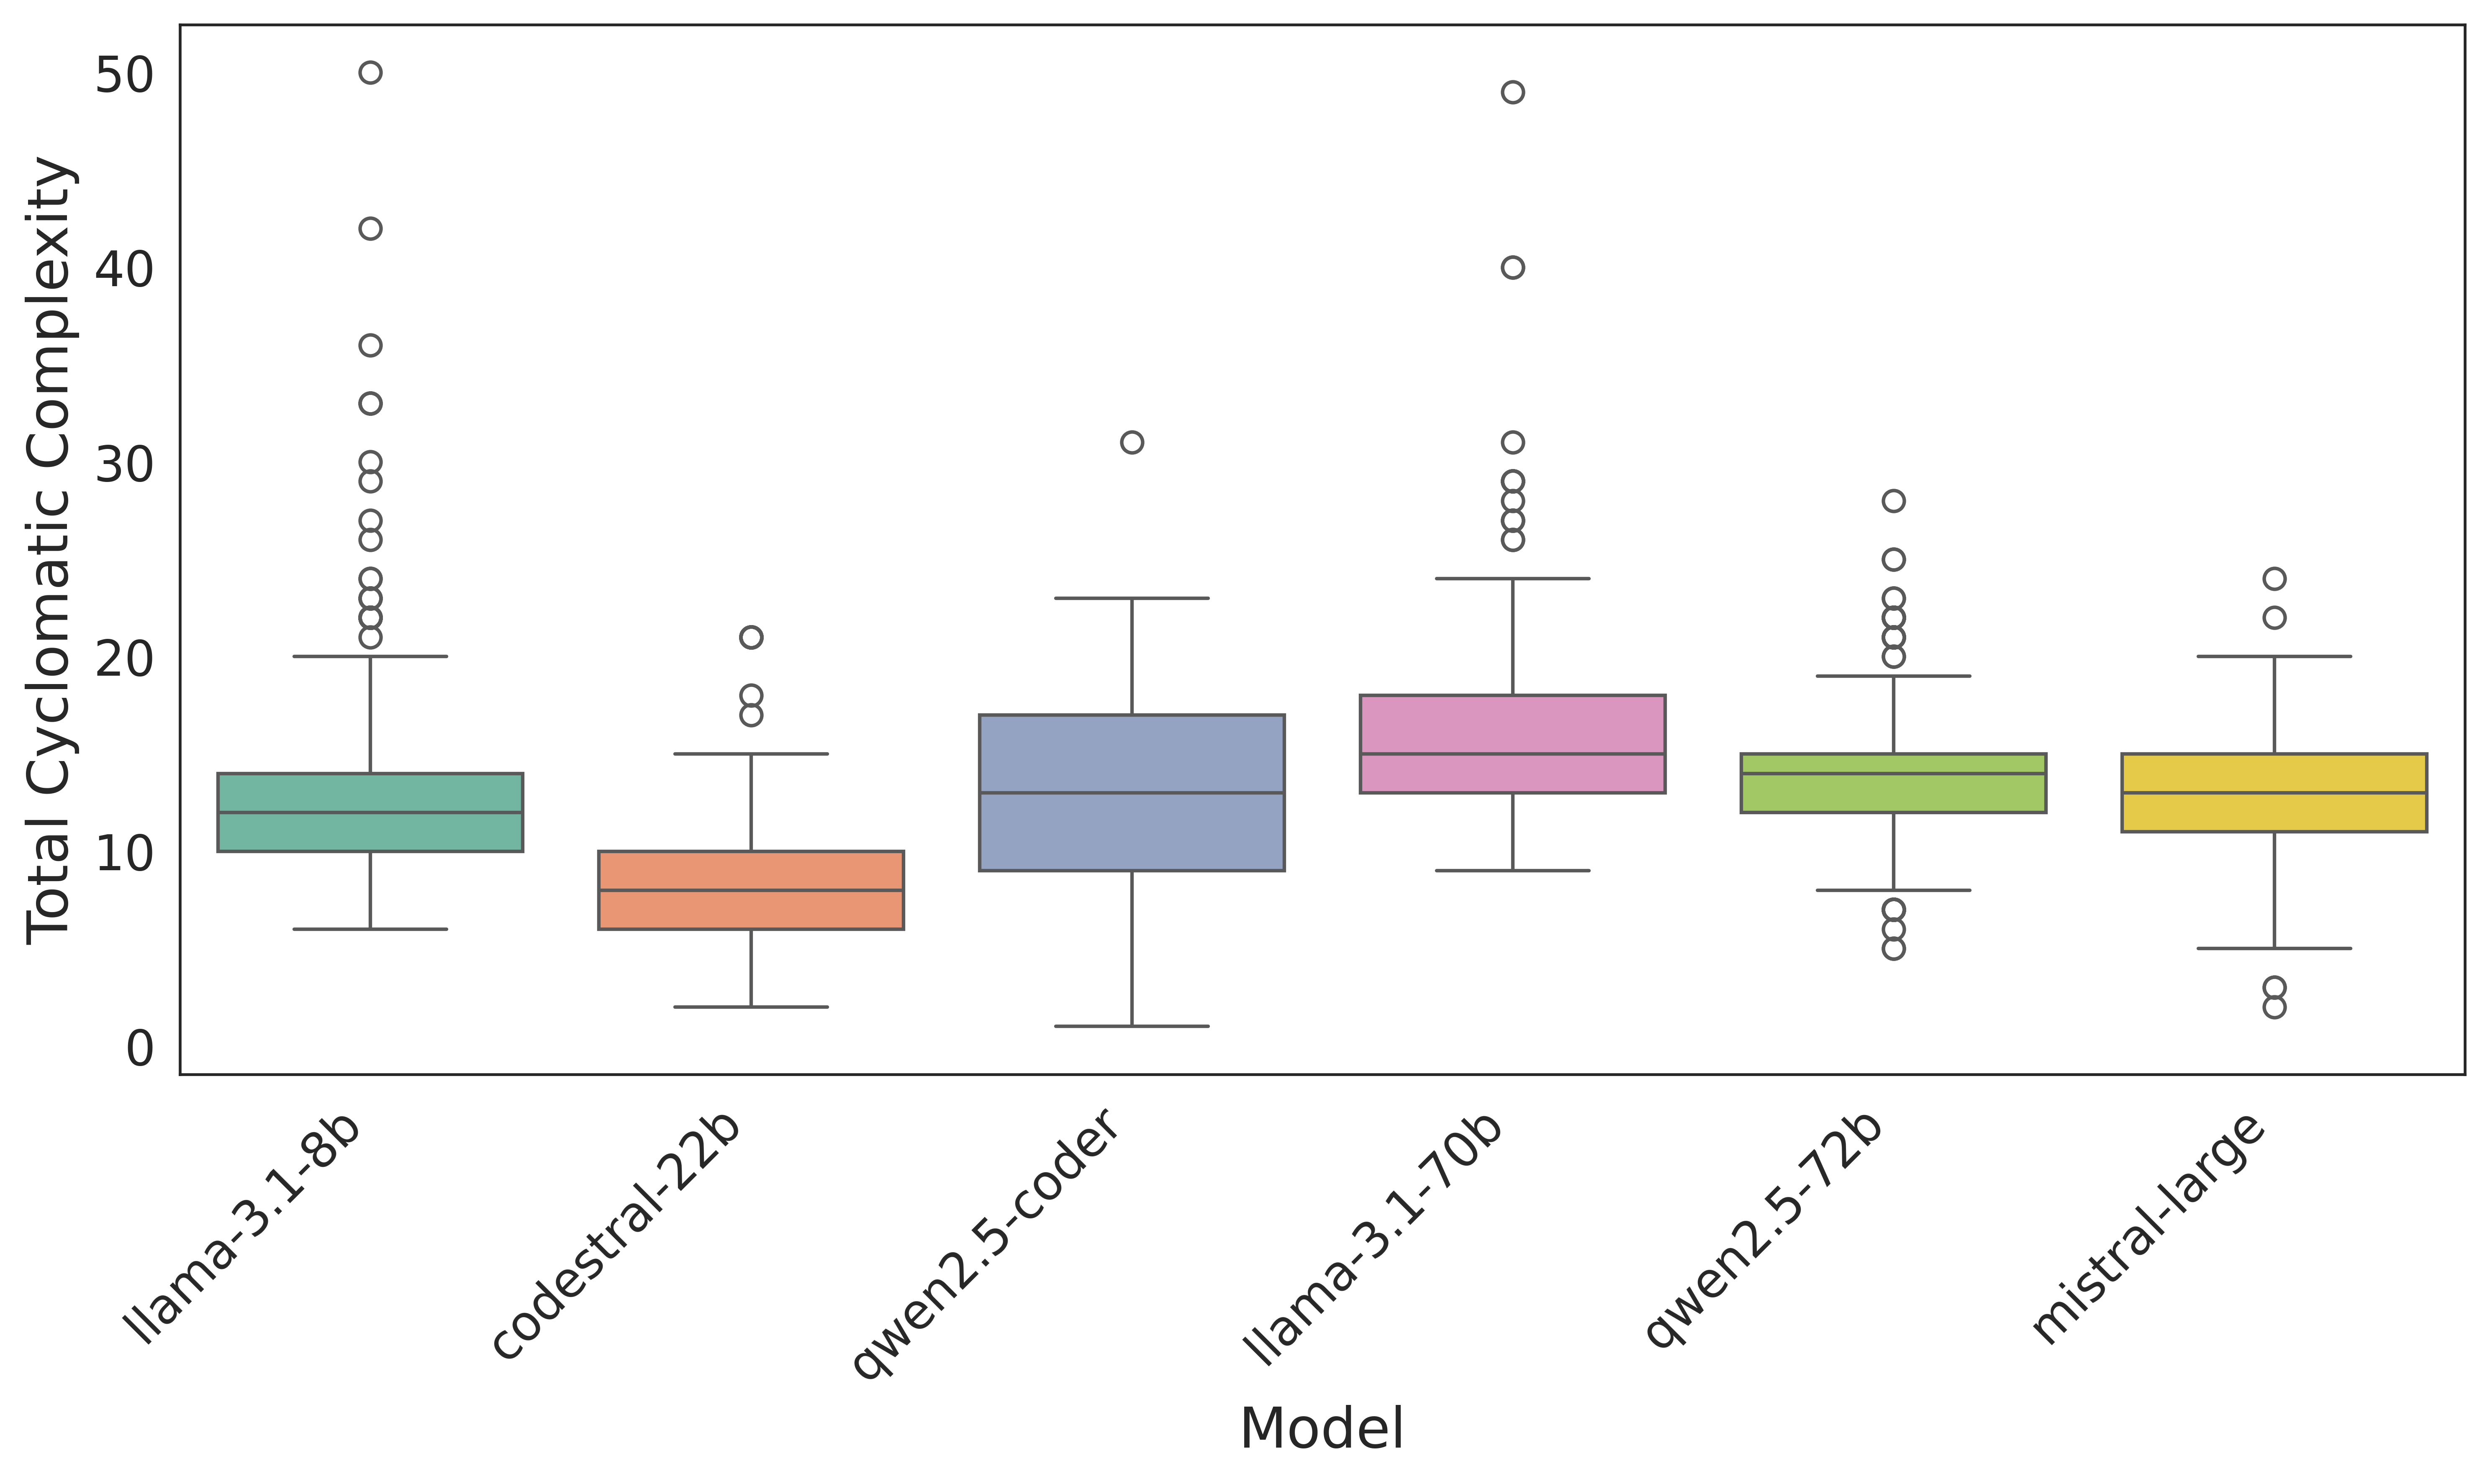
\includegraphics[width=0.65\linewidth]{img/Results/First Experimental Phase/Cyclomatic Complexity Distribution per Model.png}
    \caption[Cyclomatic complexity distribution]{\textbf{Cyclomatic complexity distribution}. Boxplot showing the distribution of total cyclomatic complexity values for each evaluated model, aggregated across all experiments.}
    \label{fig:cyc_complexity}
\end{figure}

These aforementioned Llama outliers are also visible in the overall cyclomatic complexity distribution (see Figure~\ref{fig:cyc_complexity}), with the Llama models producing both the most and the furthest outliers. While they typically generate moderately complex code, they occasionally produce exceptionally intricate solutions. The llama-3.1-70b model, in particular, maintains the highest average complexity, suggesting a consistent tendency toward more complex control flows. In contrast, codestral-22b spans the lowest complexity values. Qwen2.5-coder shows the widest boxplot yet has the fewest outliers and the lowest observed complexity, suggesting that while its code varies more in structural complexity, it generally avoids producing excessively complex scripts. Despite these distinctions, all models typically produce code with cyclomatic complexity values ranging from 1 to 24, suggesting a shared tendency to target moderately complex solutions for the given tasks.

\paragraph{Maintainability Index}\mbox{}\\

\begin{figure}[!b]
    \centering
    
\includegraphics[width=\linewidth]{img/Results/First Experimental Phase/Maintainability Index per Model.png}
    \caption[Maintainability index distribution across experiments]{\textbf{Maintainability index distribution across experiments}. Boxplots showing the distribution of maintainability index scores for each model across the three experimental setups.}
    \label{fig:MI_distribution}
\end{figure}

\noindent Codestral-22b generally achieves the highest maintainability scores, making it a reliable choice for generating maintainable code. Llama-3.1-8b follows behind, showing a clear upward trend in maintainability when robustness instructions and dynamic generation are incorporated, suggesting responsiveness to more detailed or assisting prompts. However, this improvement is accompanied by some inconsistency in output quality. Qwen2.5-coder displays more volatile performance, particularly showing a decline in maintainability with the introduction of robustness instructions but recovering somewhat under the dynamic structures, highlighting its sensitivity to prompting style and structural instructions. Llama-3.1-70b also appears sensitive to prompt and context changes, scoring relatively low in the second and third experiments, which may be linked to its tendency to generate more complex code structures. In comparison, qwen2.5-72b stands out as the lowest and one of the most stable performers in maintainability, maintaining constantly poor scores across all experiments. 

Each model behaves like it has a “comfort zone” or a characteristic maintainability profile, largely unaffected by the changes in experiment conditions (see Figure~\ref{fig:MI_distribution}). This suggests that the models have intrinsic tendencies or biases in the style and complexity of code they generate that remain consistent, regardless of the experimental prompts. This clustering behavior is noteworthy because it suggests that the choice of model likely affects maintainability more than changes in prompt engineering.

\section{Direct Contextual Prompting Experiments}

\subsection{Model Accuracy Analysis}

Injecting the data structure directly into the prompt proves more effective than using RAG in handling missing data (see Figure~\ref{fig:outcome_distribution_nodata_second}). In this setup, the robustness instructions achieve an accuracy of 35.5\%, already surpassing the augmented knowledge approach. However, 40.6\% of its responses include faulty logic. It also shows the second-highest failure rate in this experimental phase at about one in five instances. The dynamic structure generation performs relatively worse, with no correct response instances, the highest faulty logic rate at 47.7\%, and the highest inaccuracy rate at 44.5\%. Because the structure is generated dynamically, the relevant response locations are not included in the structure. The models fail to recognize this and instead focus on other files when extracting data. Nevertheless, this setup records the lowest overall failure rate. Between the two approaches, the robustness instructions appear more effective for handling missing data and directing focus toward the correct responses. Conversely, the optimized prompting experiment has the highest failure rate, with about a third of its instances resulting in failure, but also emerges as the most accurate, achieving a 57.5\% accuracy rate in handling missing data.

\begin{figure}[ht]
    \centering
    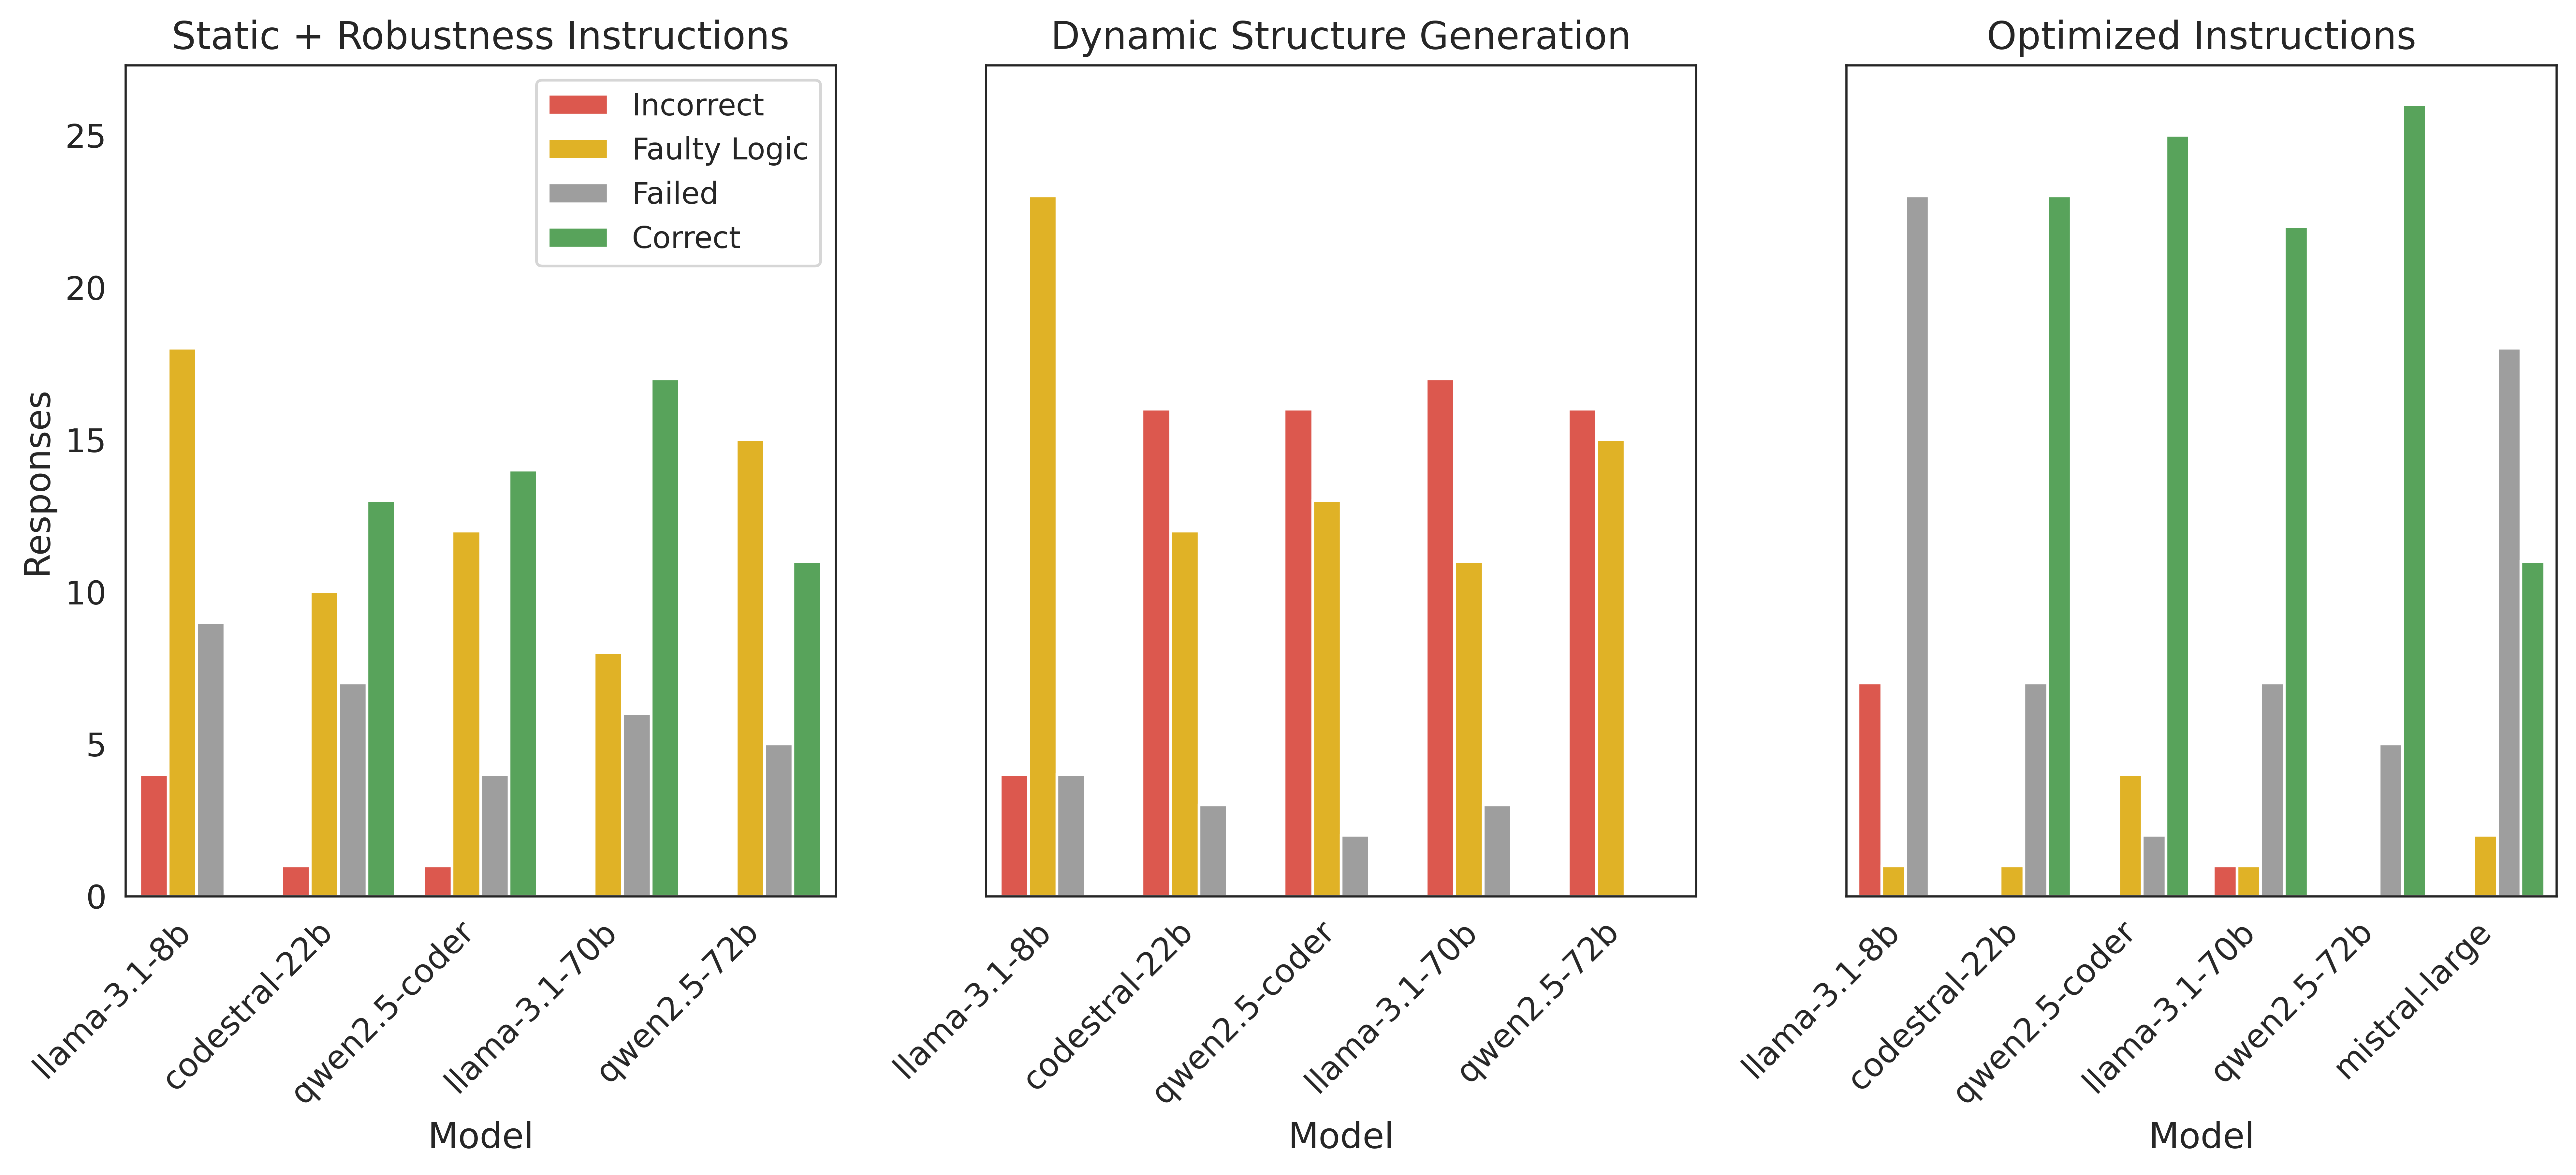
\includegraphics[width=\linewidth]{img/Results/Second Experimental Phase/Response Outcome Distribution per Model - No Data.png}
    \caption[Response outcome distribution per model when no relevant data is present]{\textbf{Response outcome distribution per model when no relevant data is present}. Each subplot corresponds to a separate experiment, showing the count of model responses grouped by their evaluation outcome.}
    \label{fig:outcome_distribution_nodata_second}
\end{figure}

From a model performance perspective, llama-3.1-8b is the weakest, with no correct responses in any of the experiments. This poor performance can be attributed to its high tendency to produce faulty logic. It is only in the third experiment that the model reduces this tendency to 3.2\%, but this is accompanied by a 74.2\% failure rate, the highest across all experiments in this phase. In the first experiment, the remaining models perform generally well in terms of accuracy, but these gains are often offset by moderate failure and inaccuracy rates. The best performers in this experiment are llama-3.1-70b, with 54.8\% of its responses being correct, and qwen2.5-coder, with 45.2\%.

Alongside llama-3.1-8b, mistral-large also records a 58.1\% failure rate in the third experiment, with these two models being the primary contributors to the experiment's overall high failure rate. Excluding them, the remaining models perform very well in terms of accuracy and show relatively low rates of faulty logic and inaccurate responses. The best performers here are qwen2.5-coder with an accuracy of 80.6\%, and qwen2.5-72b at 83.8\%, both also achieving the lowest failure rates in this experiment.

Upon execution on DDPs with the required data, llama-3.1-70b is one of the best performing models in the first two experiments. Under the robustness instructions, it achieves a complete accuracy of 44.8\% and avoids any failures entirely. However, the model still records a 42.4\% inaccuracy rate, which seems to be the defining characteristic of this experimental setup, where most models exhibit substantially higher inaccuracy rates than complete accuracy ones (see Figure~\ref{fig:outcome_distribution_data_second}). In the second experiment, model performance is more balanced, with the majority of the models achieving complete accuracy rates of 30\% or higher. The high inaccuracy trend persists here as well, though there is also a greater tendency for models to produce partially correct responses compared to the first experiment. Additionally, the dynamic structure generation notably reduces the failure rate relative to the first experiment. Despite an overall moderate performance, providing the data structure through the prompt yields better results than through the external knowledge base.

\begin{figure}[ht]
    \centering
    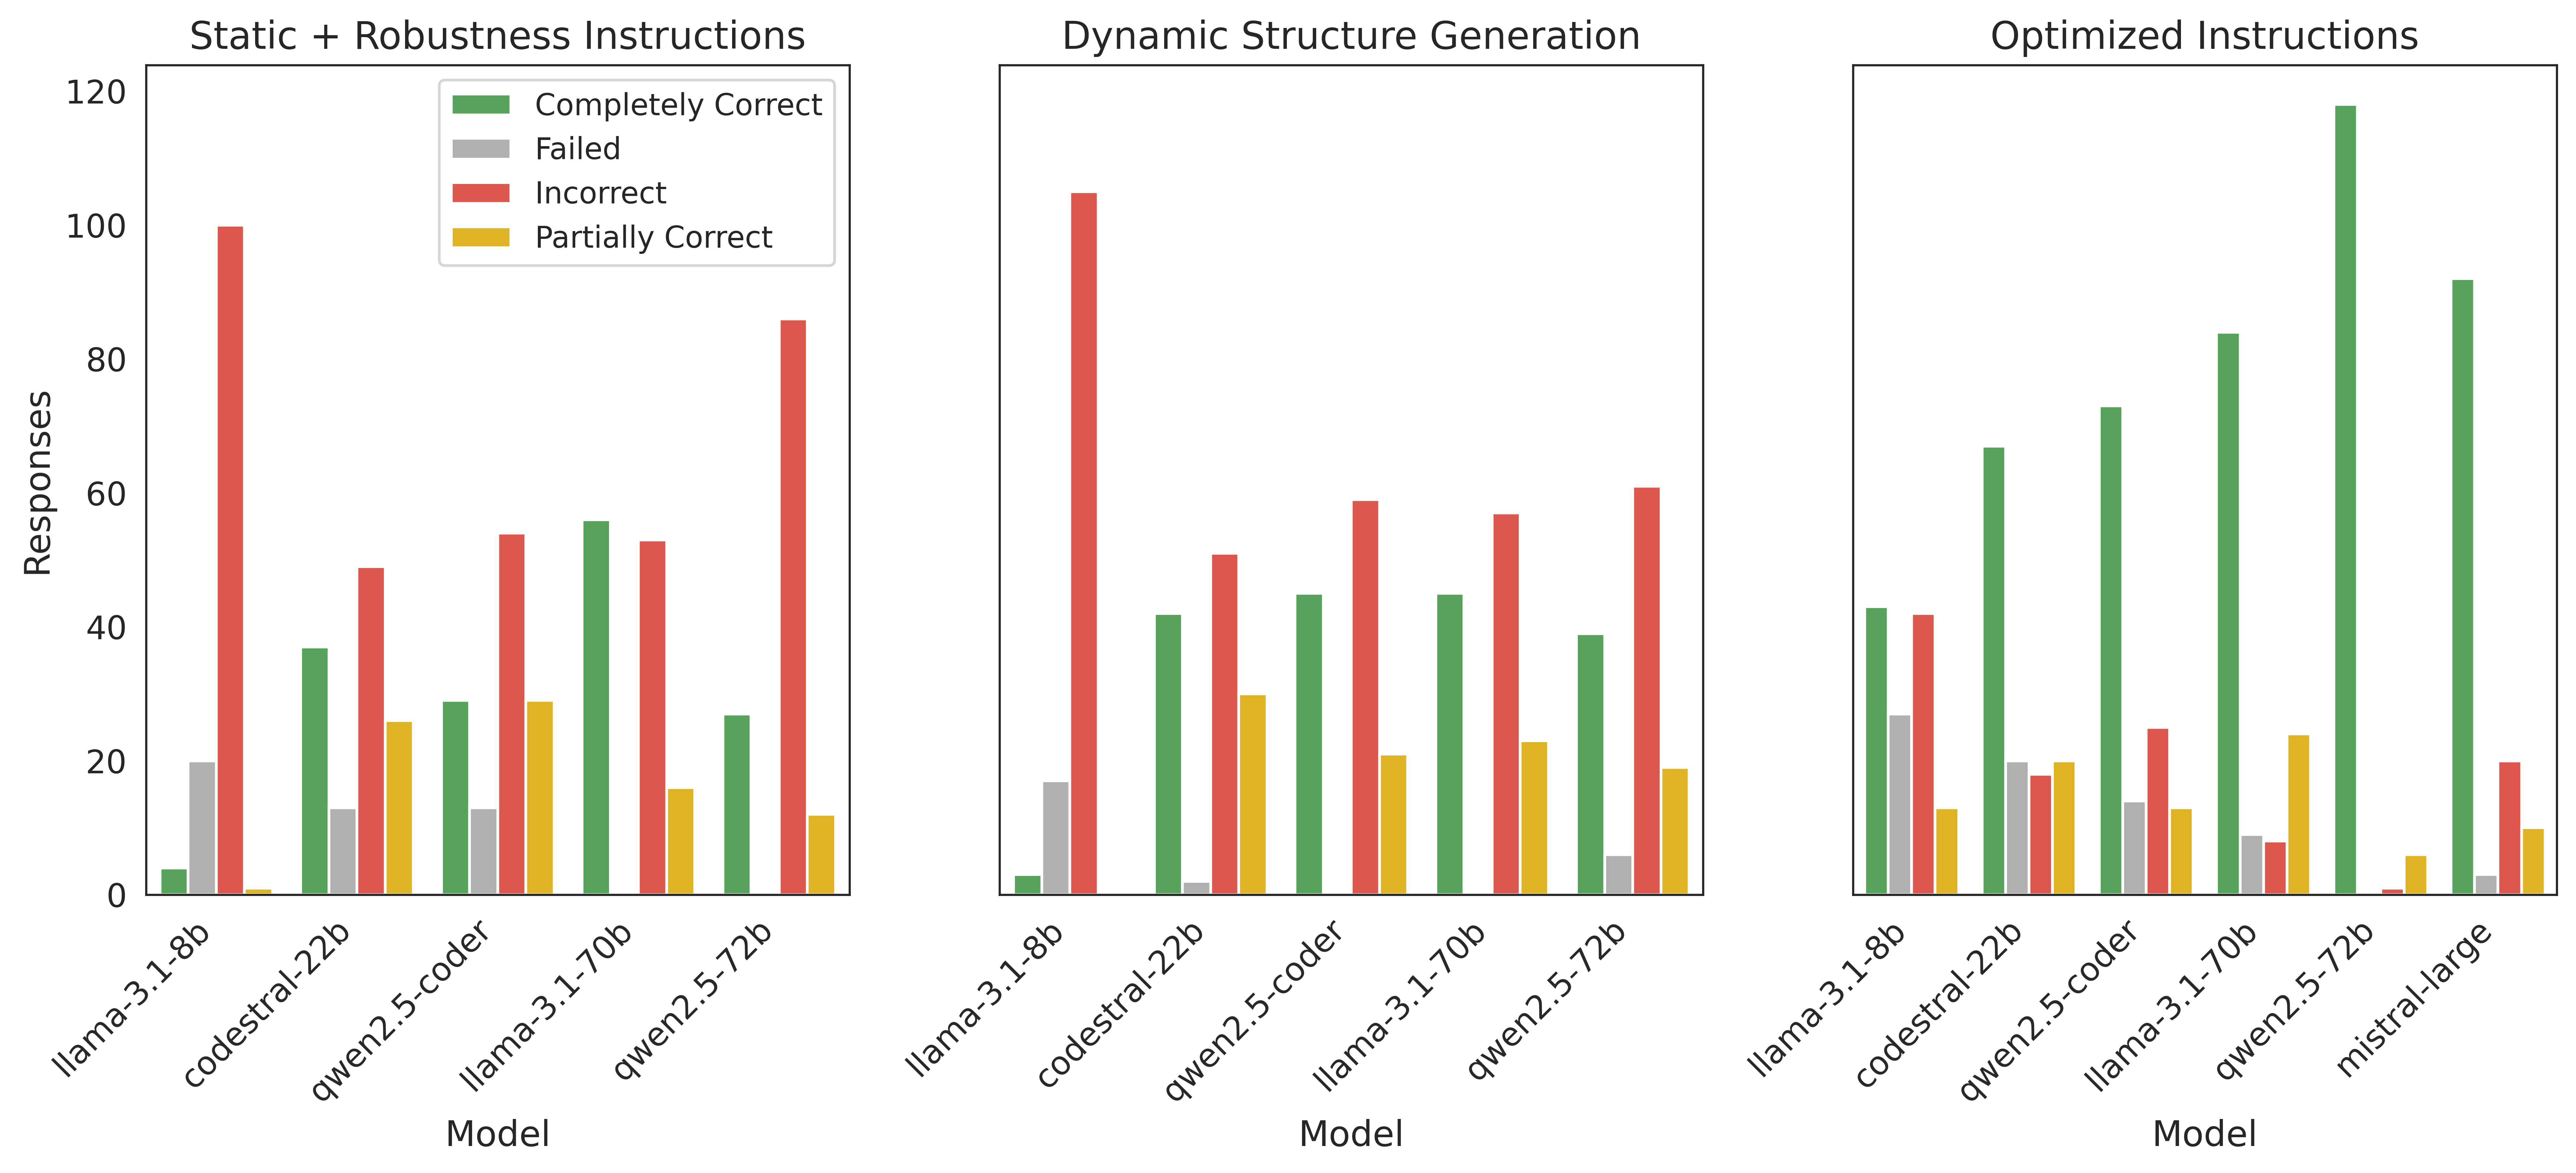
\includegraphics[width=\linewidth]{img/Results/Second Experimental Phase/Response Outcome Distribution per Model - With Data.png}
    \caption[Response outcome distribution per model when relevant data is present]{\textbf{Response outcome distribution per model when relevant data is present}. Each subplot corresponds to a separate experiment, showing the count of model responses grouped by their F1 evaluation outcome.}
    \label{fig:outcome_distribution_data_second}
\end{figure}

Except for llama-3.1-8b, which maintains its overall poor performance, all models achieve their best results in the third experiment. Among the smaller models, qwen2.5-coder stands out with a complete accuracy of 58.4\% and an inaccuracy rate of 20\%. Codestral-22b follows closely, recording a lower inaccuracy rate but a higher rate of partially correct responses and failures. In this setup, the larger models consistently outperform the smaller ones, achieving higher complete accuracy rates, lower partially correct response rates, lower inaccuracy rates, and fewer failures overall. The highest performance observed across all experiments is achieved by qwen2.5-72b, with a complete accuracy of 94.4\%, the lowest inaccuracy rate at 0.8\%, and zero failures. Interestingly, while two models record a 0\% failure rate in the first two experiments, only this model achieves it in the third one. Mistral-large and llama-3.1-70b follow in terms of complete accuracy at 73.6\% and 67.2\%, respectively, but are held back by their higher tendencies to produce partially correct or inaccurate responses. Overall, the Qwen models achieve the highest performance within their respective size categories in successfully extracting information.

\paragraph{Precision, Recall, and F1 Score Performance}\mbox{}\\

\noindent For the second and third experiments, most models display moderate performance, with accuracy metrics generally ranging between 0.40 and 0.57. Similar to the response analysis, in the first experiment, llama-3.1-70b is the best performer. The qwen2.5-72b exhibits relatively poor performance compared to the other models, with the smaller llama-3.1-8b remaining the worst performer. In the second experiment, we again observe a more balanced and similar performance among most models. A consistent trend across both experimental phases is that the models' recall is higher than their precision, suggesting that the tendency to overestimate responses is an inherent model behavior rather than a consequence of the instructions provided.

\begin{figure}[ht]
    \centering
    \includegraphics[width=\linewidth]{img/Results/Second Experimental Phase/Evaluation of Model Performance Across Experiments.png}
    \caption[Model performance across non-failed experimental instances]{\textbf{Model performance across non-failed experimental instances}. Each subplot represents a distinct experiment, illustrating model performance variations with respect to precision, recall, and F1 score.}
    \label{fig:model_performance_nonfailed_second}
\end{figure}

Even with the reduced context size alongside the optimized instructions, llama-3.1-8b fails to surpass the moderate performance exhibited by other models in previous experiments. For the smaller models, although qwen2.5-coder performs better in the response analysis, it is overtaken by codestral-22b in terms of precision, recall, and F1 score. As observed in Figure~\ref{fig:model_performance_nonfailed_second}, qwen2.5-72b achieves near-perfect performance in the third experiment, with scores of 0.99 across all metrics. The larger models generally lead the rankings, with llama-3.1-70b as the second-best performer and mistral-large as the third-best. However, the largest models within each size category are not the top performers, suggesting again that model size is not the determinant for better performance. Across the majority of models, recall remains slightly higher than precision and F1, though the discrepancies are relatively small, resulting in a fairly balanced overall performance.

The models' unreliable and erratic performance, reflected in the relatively high standard deviation values, persists in the first and second experiments (see Table~\ref{tab:F1_and_st_deviation_second}). While the F1 scores are improved and the variance is somewhat reduced in the third experiment, the smaller models and the mistral-large still demonstrate high variation tendencies. The only model we can confidently rely on in terms of high accuracy and consistency is the qwen2.5-72b under the optimized instructions.

\begin{table}[h]
    \centering
    \renewcommand{\arraystretch}{1.2}
    \setlength{\tabcolsep}{10pt}
    \begin{tabular}{lccc}
        \hline
        \textbf{Model} & 
        \makecell{\textbf{Static + Robustness} \\ \textbf{Instructions}} & 
        \makecell{\textbf{Dynamic Structure} \\ \textbf{Generation}} & 
        \makecell{\textbf{Optimized} \\ \textbf{Instructions}} \\
        \hline
        llama-3.1-8b & \cellcolor{red!15} $0.04 \pm 0.19$ & \cellcolor{red!15} $0.03 \pm 0.17$ & \cellcolor{red!15} $0.53 \pm 0.48$ \\
        codestral-22b & $0.47 \pm 0.47$ & $0.49 \pm 0.47$ & $0.76 \pm 0.39$ \\
        qwen2.5-coder & $0.45 \pm 0.46$ & $0.47 \pm 0.48$ & $0.72 \pm 0.43$ \\
        llama-3.1-70b & $0.55 \pm 0.49$ & $0.49 \pm 0.48$ & $0.88 \pm 0.28$ \\
        qwen2.5-72b & $0.29 \pm 0.44$ & $0.44 \pm 0.48$ & \cellcolor{green!20} $0.99 \pm 0.09$ \\
        mistral-large & – & – & $0.83 \pm 0.37$ \\
        \hline
    \end{tabular}
    \caption[Model F1 score performance and consistency]{\textbf{Model F1 score performance and consistency}. This table provides an overview of the mean F1 scores and standard deviations for each model under the three experimental conditions.}
    \label{tab:F1_and_st_deviation_second}
\end{table}

\paragraph{Model Answering Behavior}\mbox{}\\

\noindent When analyzing the distribution of non-failed response types (see Figure~\ref{fig:answer_type_classification_second}), the models in both the first and second experiments exhibit relatively low perfect match rates, at 26.4\% and 29\% respectively. In both cases, more than a third of their responses are empty files. Another common pattern is the extraction of data from incorrect files, which occurs in approximately 21\% of the generated responses. The highest proportion of perfect match answers is achieved by codestral-22b (33.6\%) and llama-3.1-70b (40.4\%), while the remaining models display stronger tendencies toward incorrect outputs that follow the common inaccuracy patterns. Qwen2.5-coder follows closely with 31.2\% perfect matches, but also has the highest rate (18.6\%) of including additional, unnecessary records in its responses.

\begin{figure}[ht]
    \centering
    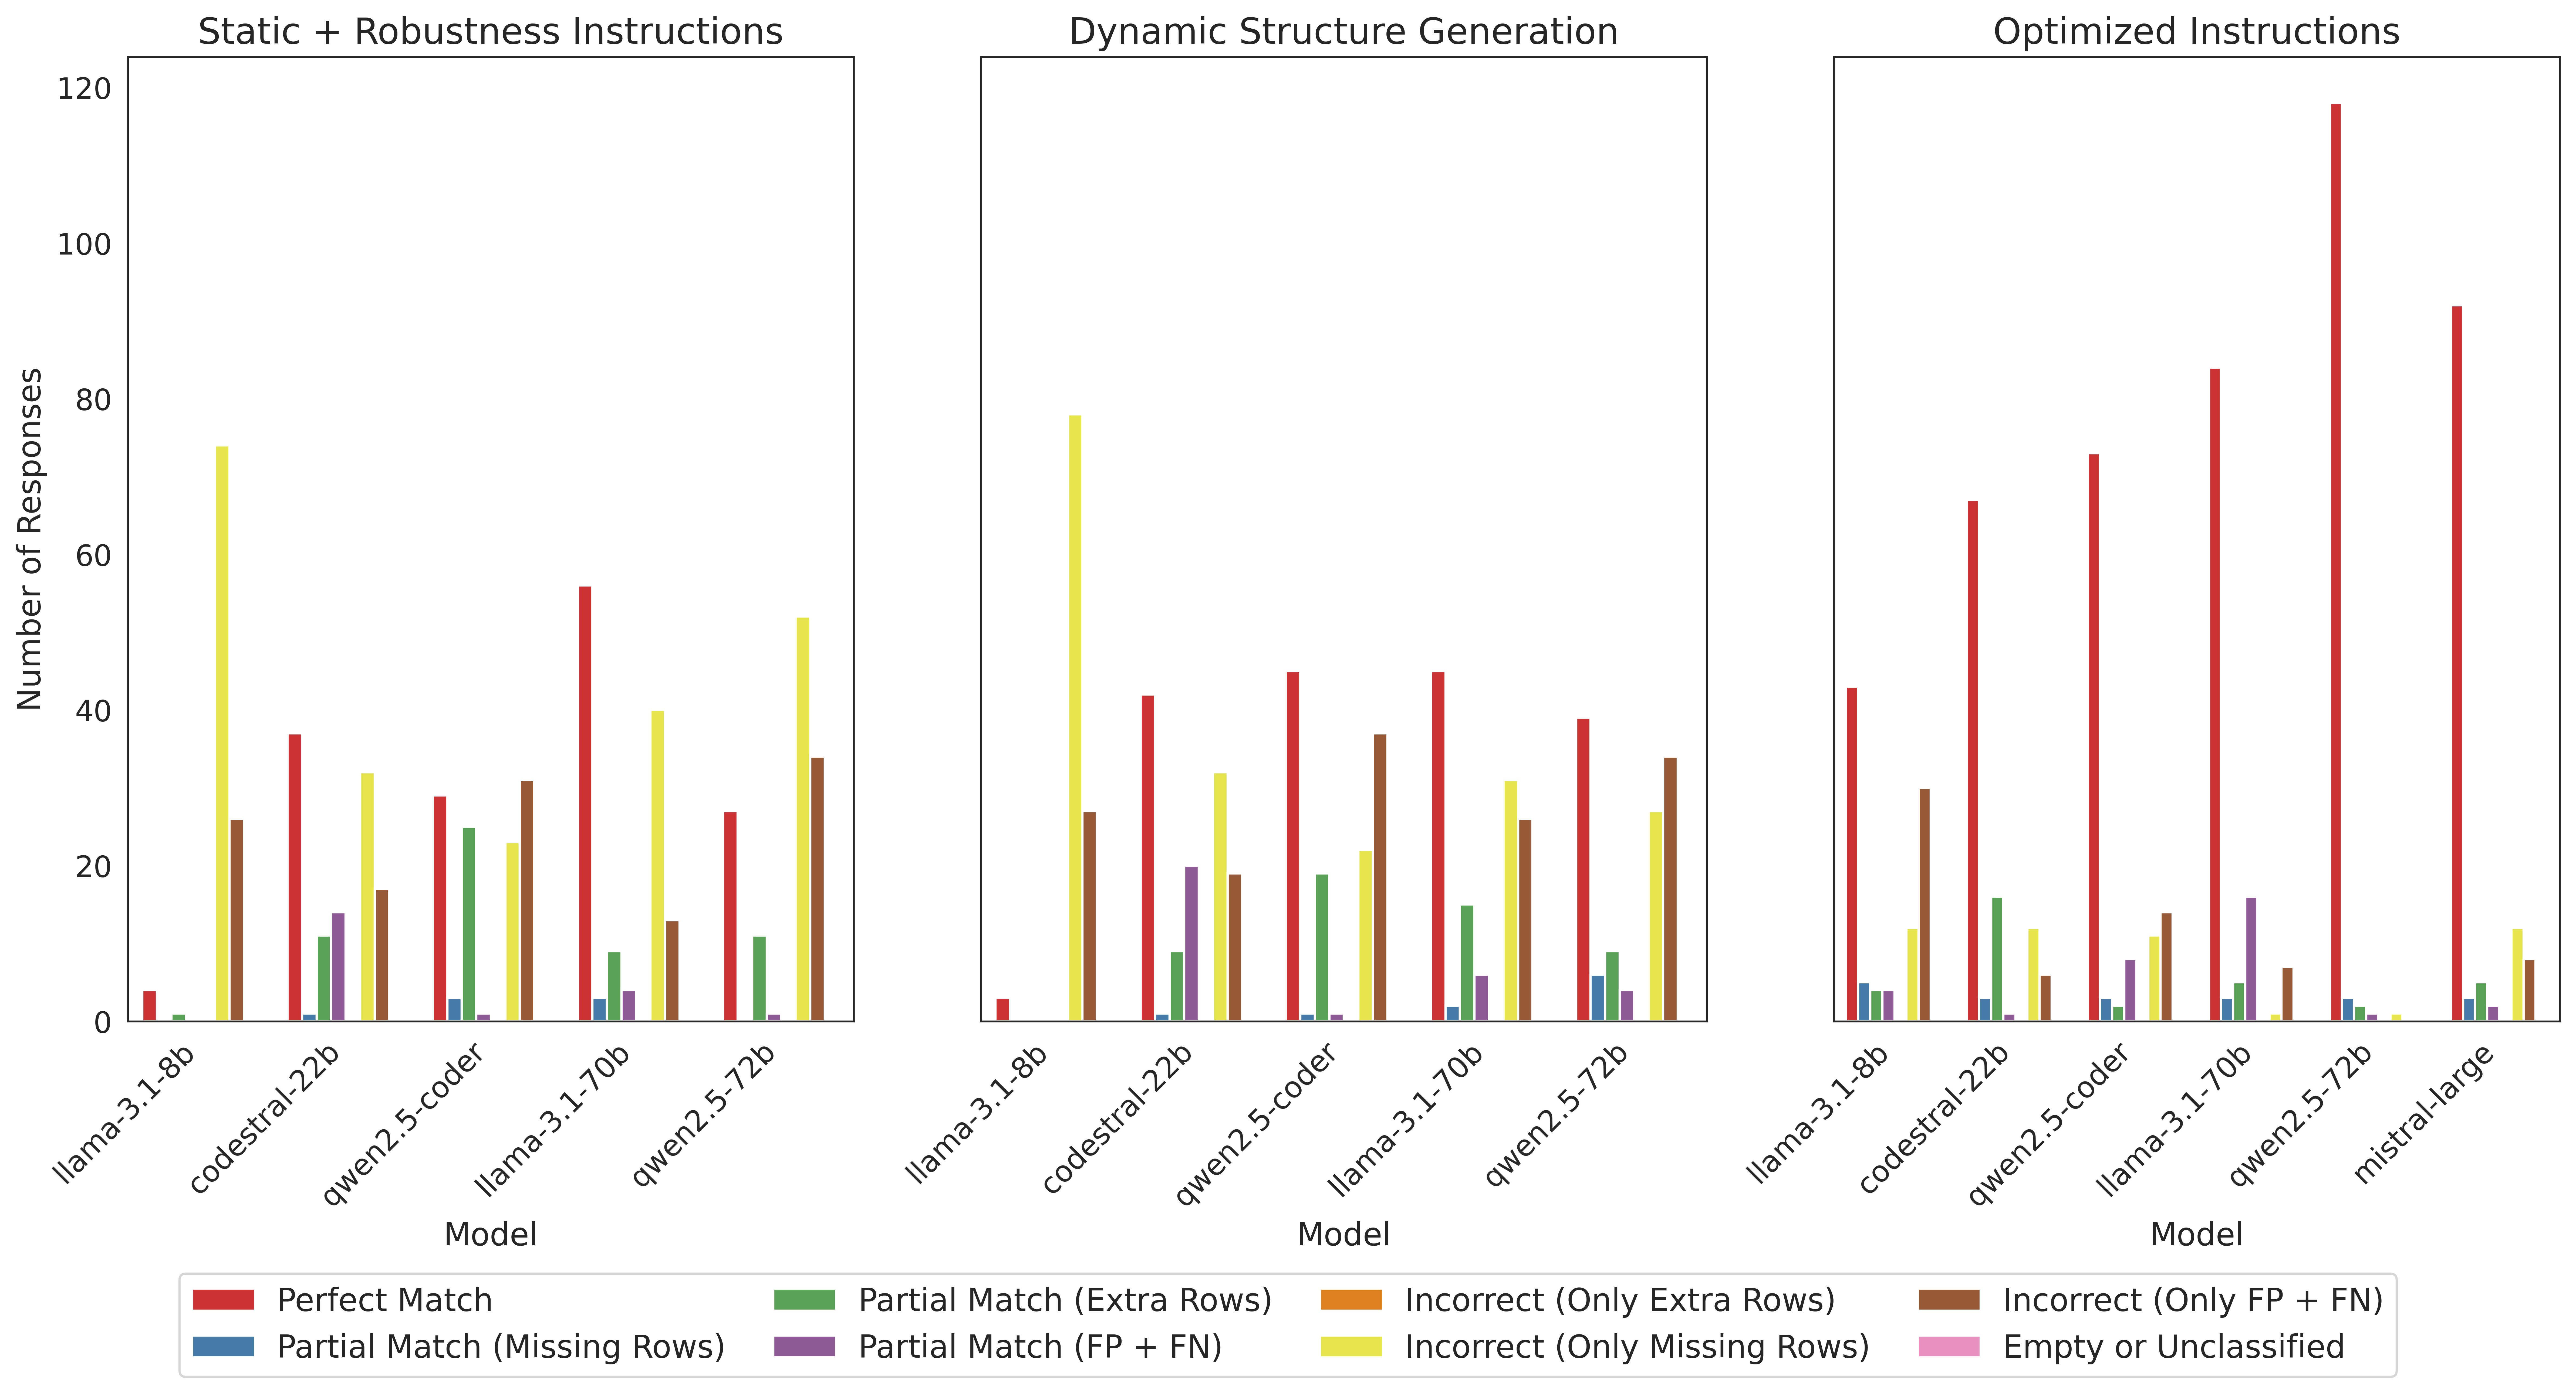
\includegraphics[width=\linewidth]{img/Results/Second Experimental Phase/Answer Type Classification per Model Across Experiments.png}
    \caption[Distribution of answer types by model and experimental setup]{\textbf{Distribution of answer types by model and experimental setup}. Each subplot represents a distinct experiment, illustrating the distribution of response types for each model. Responses are categorized into Perfect Matches, Partial Matches (with subtypes for missing or extra rows), and Incorrect outcomes (with subtypes for extra, missing, or both types of inaccurate rows).}
    \label{fig:answer_type_classification_second}
\end{figure}

The optimized instructions setup achieves the highest perfect match rate at 70.5\%, while maintaining very low rates across other response classes. Under these conditions, codestral-22b overestimates its responses in 15.2\% of cases, whereas qwen2.5-coder tends to focus on incorrect records in 12.6\% of cases. Among the larger models, llama-3.1-70b shows the highest tendency (13.8\%) to partially extract correct data before including additional records in its responses.

Interestingly, despite the optimized instructions explicitly specifying where to focus and what to extract from each file, such deviations still occur across all of the selected models. This suggests that the discrepancies in this experiment stem primarily from faulty data extraction and erroneous processing. Another likely cause is the models misinterpreting the provided instructions in the prompt. Even the best performing model is not free from these types of minor errors, even if at a diminutive rate.

\paragraph{Question-wise Model Comparative Analysis}\mbox{}\\

\noindent Providing the DDP structure via prompts helps in expanding the range of questions the models can successfully answer. As shown in Figure~\ref{fig:f1_score_heatmap_second}, the number of problematic questions has been reduced to only questions 5, 6, 7, and 8, although some models are still able to answer them in certain instances. It appears that in this phase, models struggle with temporal tracking and extracting data from specific files. This suggests that the difficulty the models face is not directly related to how the questions are phrased. Furthermore, the same phenomenon observed previously, where models are able to answer more questions but lose accuracy when switching from robustness instructions to dynamic structure generation, is apparent here as well, particularly emphasized for the early questions.

\begin{figure}[ht]
    \centering
    \includegraphics[width=\linewidth]{img/Results/Second Experimental Phase/F1 Score Heatmaps (Model × Question).png}
    \caption[F1 score heatmaps by model and question across experiments]{\textbf{F1 score heatmaps by model and question across experiments}. Each heatmap represents a distinct experiment, illustrating the model performance per question. Higher scores (darker shades of red) indicate better model accuracy for that question-experiment pair.}
    \label{fig:f1_score_heatmap_second}
\end{figure}

It is important to emphasize that in the third experiment, the optimized instructions address all external weaknesses identified in the previous experiments. These instructions provide context on the paths of relevant files, specify which fields from the JSON objects the models should focus on for particular parts of the response, and provide only the relevant JSON object structures instead of the full DDP scope. This high level of guidance explains the strong performance observed. As such, any model with poor results in this experiment likely represents a particularly weak performance or a candidate for exclusion in future research within the scope of this study. Interestingly, some models still struggle with questions they had previously answered more accurately in earlier experiments. It can also be observed that performance in this experiment generally improves with model size, up to mistral-large, with larger models answering more questions or performing better on specific ones than smaller models. Figure~\ref{fig:f1_score_heatmap_second} also highlights the exceptional accuracy of qwen2.5-72b compared to the rest of the selected models.

\paragraph{Retries and Their Impact on Performance}\mbox{}\\

\noindent Upon examining the models' retries (see Table~\ref{tab:retry_mean_and_st_deviation_second}), it can be observed that across all experiments, the models generally require fewer retries to produce executable code compared to the RAG approach. Most of the models show relatively low averages of retry attempts, with only the codestral-22b and llama-3.1-8b reaching approximately 1 and 2 retries on certain experiments. An interesting observation is that in the final experiment, models generally require more retries than in the previous experiments to generate a valid response. Nevertheless, the high volatility and inconsistency in the number of retries across models persist in this experimental phase as well.

\begin{table}[h]
    \centering
    \renewcommand{\arraystretch}{1.2}
    \setlength{\tabcolsep}{10pt}
    \begin{tabular}{lccc}
        \hline
        \textbf{Model} & 
        \makecell{\textbf{Static + Robustness} \\ \textbf{Instructions}} & 
        \makecell{\textbf{Dynamic Structure} \\ \textbf{Generation}} & 
        \makecell{\textbf{Optimized} \\ \textbf{Instructions}} \\
        \hline
        llama-3.1-8b & $1.29 \pm 2.06$ & $1.53 \pm 2.03$ & $2.40 \pm 2.46$ \\
        codestral-22b & $1.02 \pm 1.77$ & $0.40 \pm 1.01$ & $1.18 \pm 2.03$ \\
        qwen2.5-coder & $0.59 \pm 1.66$ & $0.12 \pm 0.39$ & $0.67 \pm 1.82$ \\
        llama-3.1-70b & $0.22 \pm 0.43$ & $0.31 \pm 0.53$ & $0.58 \pm 1.46$ \\
        qwen2.5-72b & $0.17 \pm 0.40$ & $0.32 \pm 1.18$ & $0.27 \pm 0.58$ \\
        mistral-large & – & – & $0.92 \pm 1.84$ \\
        \hline
    \end{tabular}
    \caption[Summary of model retries across experiments]{\textbf{Summary of model retries across experiments}. The average number of execution attempts and the standard deviation for each model across the experimental setups.}
    \label{tab:retry_mean_and_st_deviation_second}
\end{table}

\begin{figure}[ht]
    \centering
    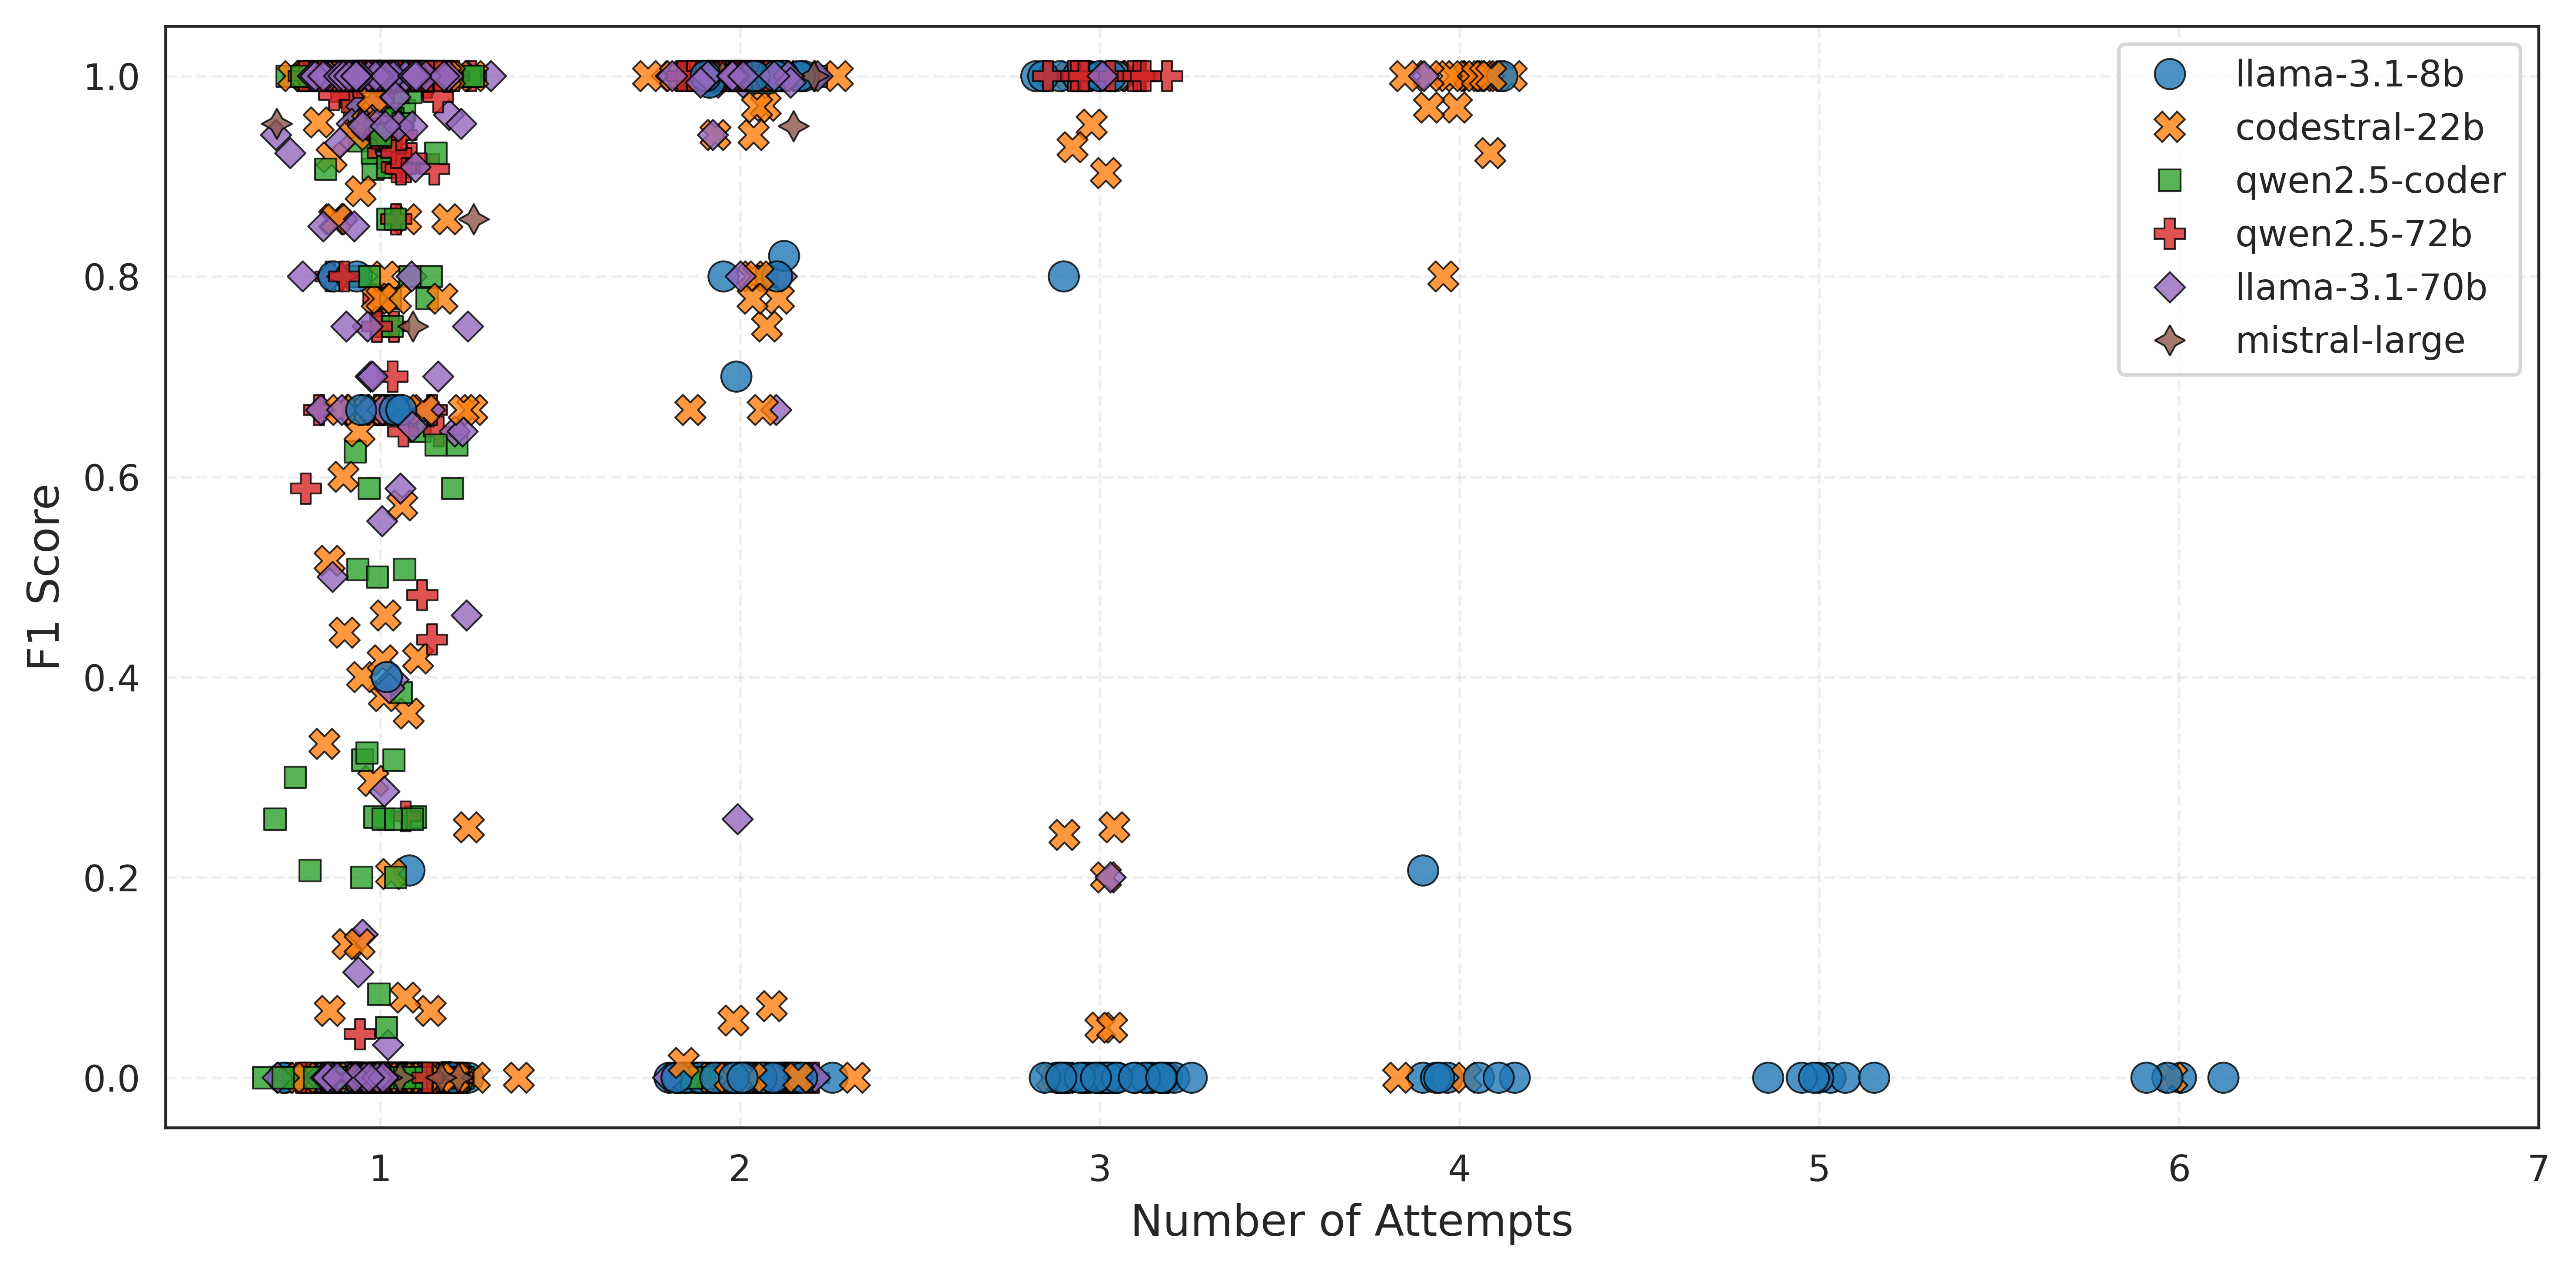
\includegraphics[width=\linewidth]{img/Results/Second Experimental Phase/Number of Retries vs F1 Score.png}
    \caption[Number of attempts vs. F1 score across models]{\textbf{Number of attempts vs. F1 score across models}. This scatter plot illustrates the relationship between the number of retries (attempts) and the achieved F1 score for various models evaluated across all experiments. Each point represents an individual experimental instance, with a slight jitter applied to improve visibility. Different colors and markers distinguish the models to facilitate comparison. The x-axis shows the total number of attempts (initial attempt plus retries).}
    \label{fig:retries_vs_F1_second}
\end{figure}

In a similar fashion to the RAG-enhanced queries, the majority of responses in this phase are concentrated on the very first execution attempt. Here, however, we observe a greater number of highly accurate outputs occurring in some of the subsequent attempts. As shown in Figure~\ref{fig:retries_vs_F1_second}, large clusters of high F1 scores can be seen in the second, third, and fourth attempts. In contrast, the fifth and sixth attempts are primarily associated with scores of 0. Notably, the model most frequently appearing with an F1 score of 0 in these later attempts is the llama-3.1-8b. An interesting observation is that when models require more attempts to generate a valid response, their performance tends to be polarized, producing either very low scores or very high scores. Particularly on the third and fourth attempts, there are no records of models performing moderately, only the two mentioned extremes. In contrast, the widest variety of responses in terms of accuracy is concentrated on the very first attempt. Based on these results, a suggested minimum retry limit would be four attempts, as many models achieve high F1 scores within this range, while the majority of the larger models tend to peak in earlier attempts. These patterns suggest that while additional retries can recover performance for specific models in a prompt-focused setup, others may not benefit meaningfully beyond the first few attempts.

\subsection{Error Analysis}

The frequency of FileNotFoundError occurrences has been significantly reduced in this experimental phase. As shown in Figure~\ref{fig:error_frequency_second}, it remains the most common type of runtime errors overall, but its actual frequency is much lower compared to the RAG experiments. For many models, other issues, such as AttributeError or TypeError, occur more frequently than FileNotFoundError. This shift suggests that faulty path generation is a problem primarily linked to providing the data structure via RAG, rather than a persistent weakness across all prompting approaches.

\begin{figure}[ht]
    \centering
    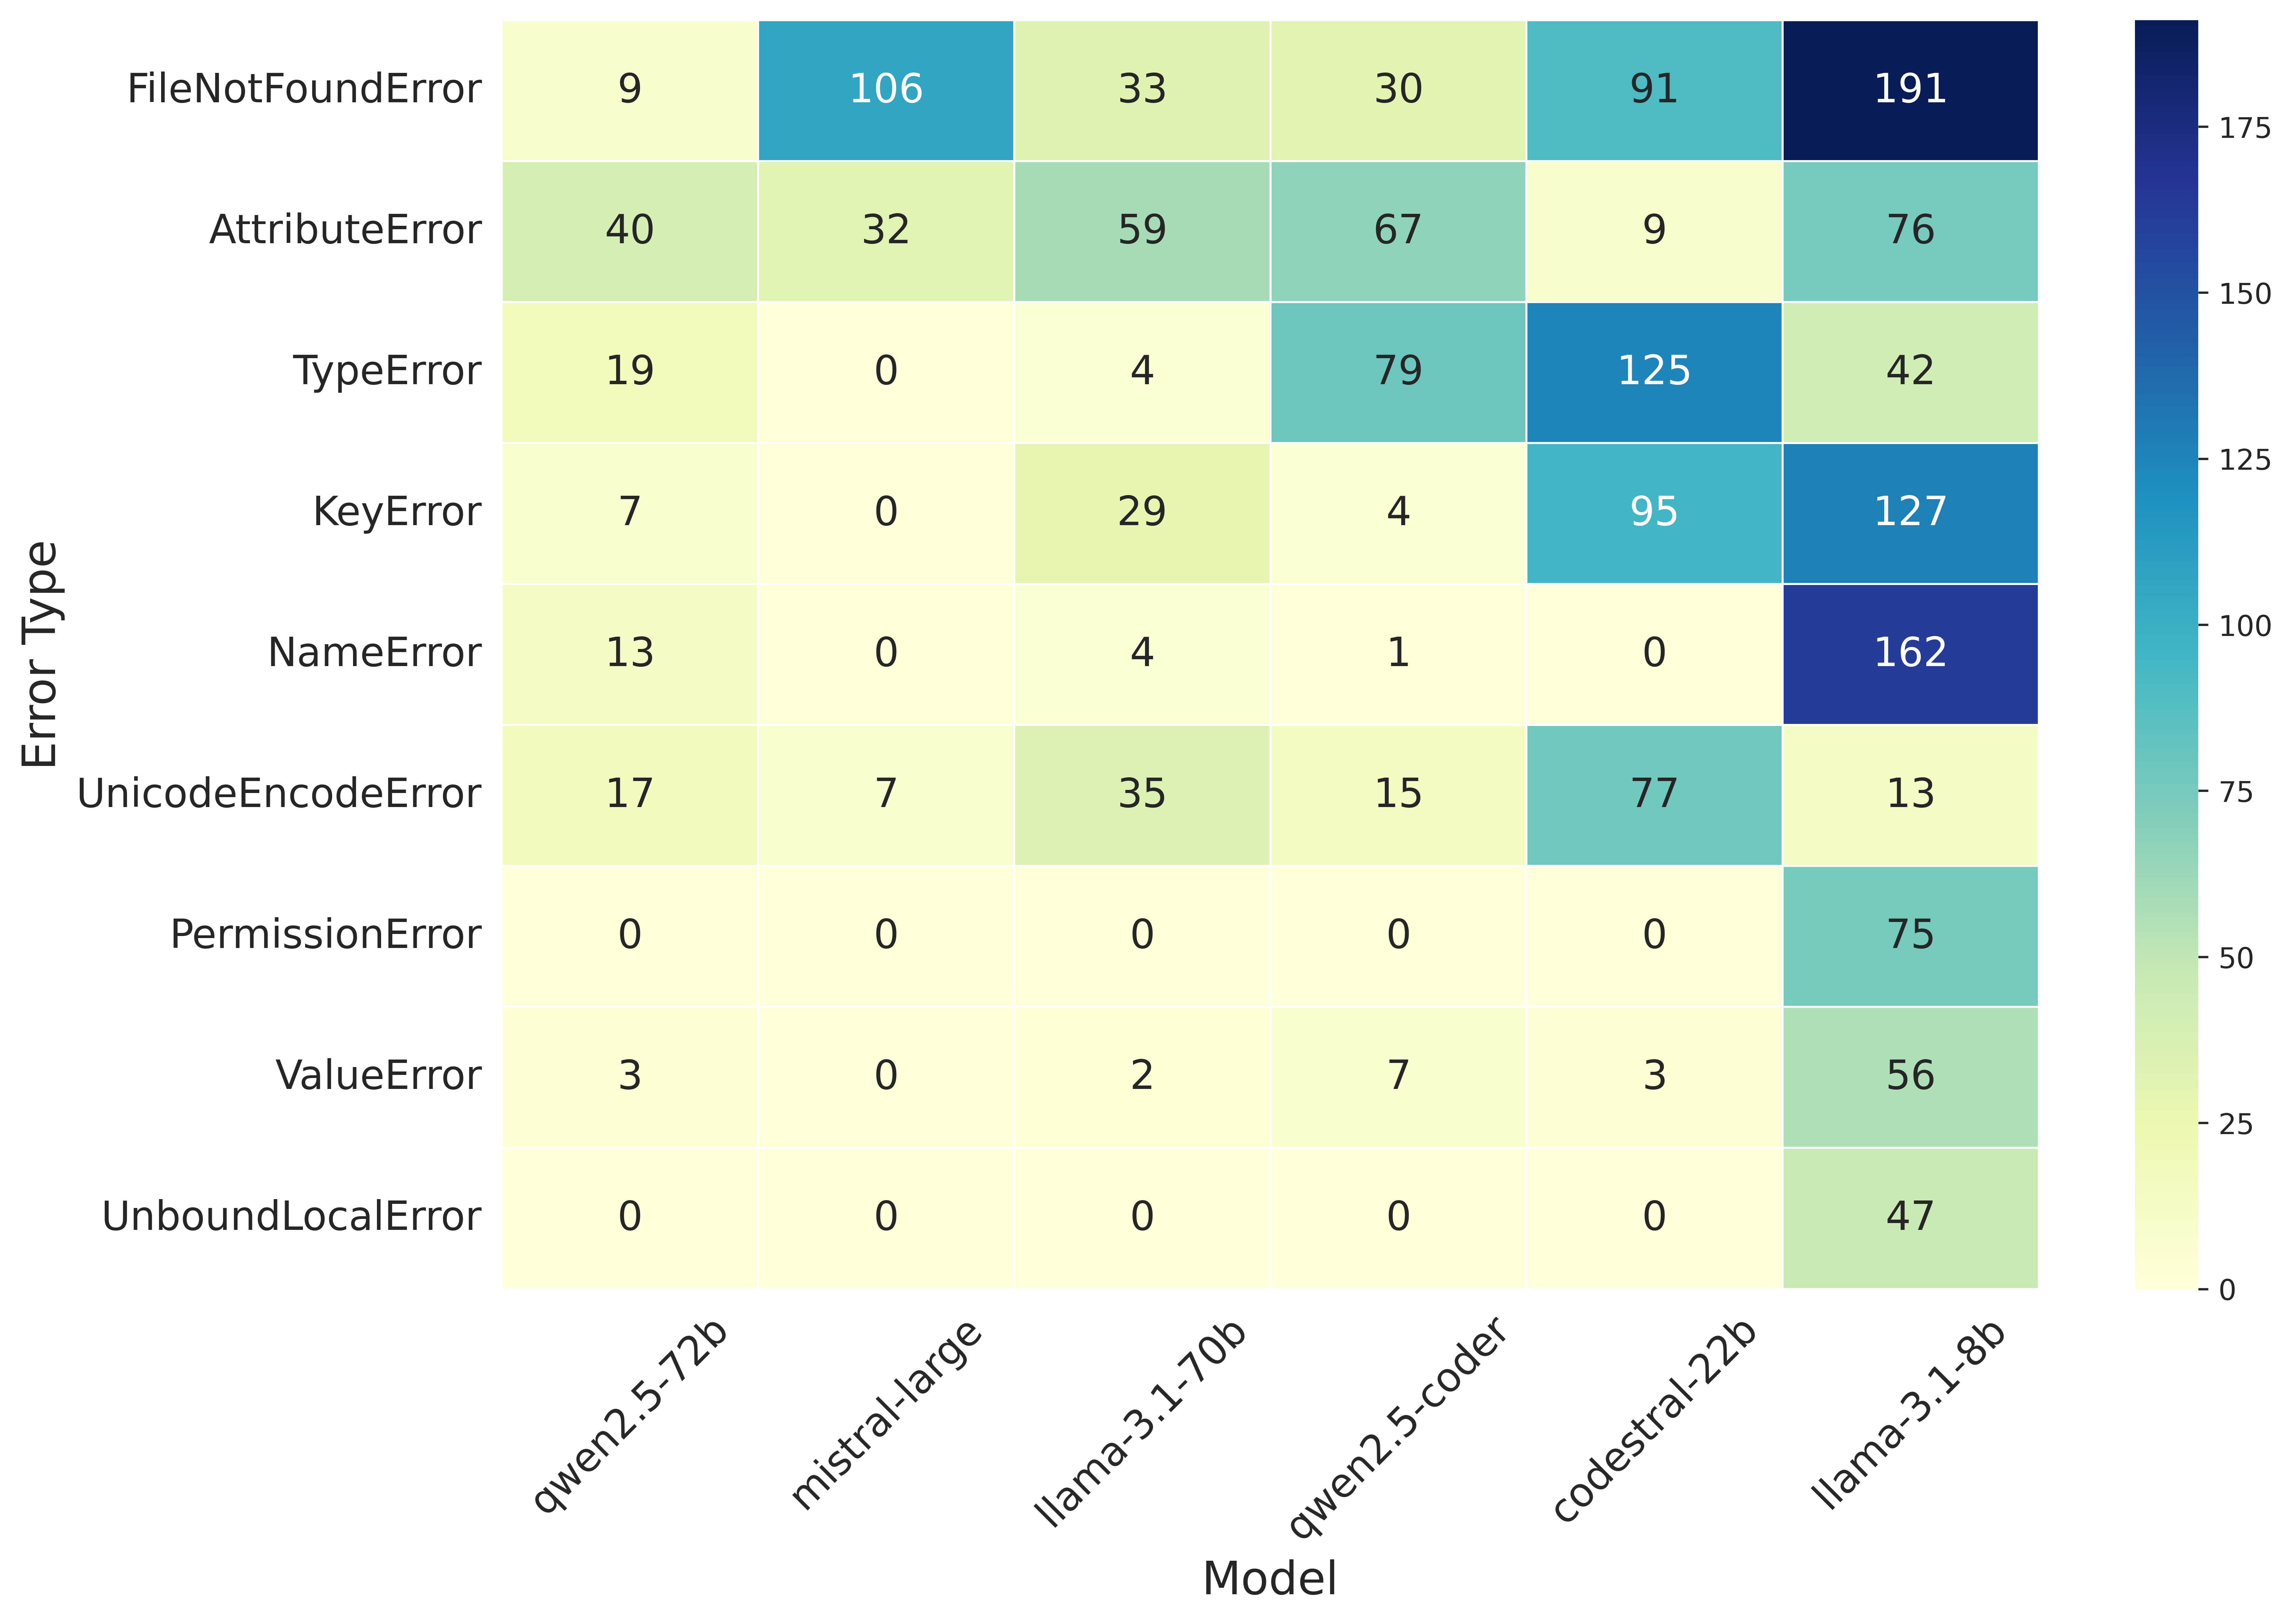
\includegraphics[width=0.80\linewidth]{img/Results/Second Experimental Phase/Error Type Frequency per Model.png}
    \caption[Error type frequency per model]{\textbf{Error type frequency per model}. Heatmap showing the frequency of the nine most common error types across all evaluated models, aggregated from all experiments. Each cell represents the number of occurrences for a given error type–model pair, with color intensity indicating frequency. Models are ordered from lowest to highest total error count, and error types are ranked from most to least frequent.}
    \label{fig:error_frequency_second}
\end{figure}

The persistent error types in this phase largely mirror those encountered in the first phase, as shown in Figure~\ref{fig:error_frequency}, with ParserError and SyntaxError also appearing frequently. However, the gap between the likelihood of experiencing these errors and encountering a FileNotFoundError on the first generation attempt has narrowed considerably. In the first phase, this difference reached up to about 500 instances, whereas in the second phase, it has dropped to just 39. Interestingly, issues related to processing or successfully extracting data from the Instagram DDPs appear slightly more common in this phase compared to the first one.

The smaller models appear more prone to errors, contributing a significant portion of the total runtime issues in this task. In general, the smaller the model size, the higher the likelihood that its generated scripts produces runtime errors. The models that struggle the most with the FileNotFoundError in this phase are mistral-large and llama-3.1-8b. Interestingly, mistral-large's errors are almost exclusively of this type, showing a very low frequency for other error categories. It is worth noting that this model appears only in the optimized instructions experiment, yet it still accounts for a substantial number of errors. This suggests that its overall performance may have been considerably worse had it participated in the other experiments as well. In contrast, other models show difficulties that are concentrated in different error categories. For instance, llama-3.1-70b often fails to extract fields from JSON objects, while qwen2.5-coder struggles with correctly identifying and handling data structures, frequently confusing strings with dictionaries. The qwen2.5-72b model produces the fewest errors overall, but occasionally mistakes lists and strings for dictionaries.

\begin{figure}[ht]
    \centering
    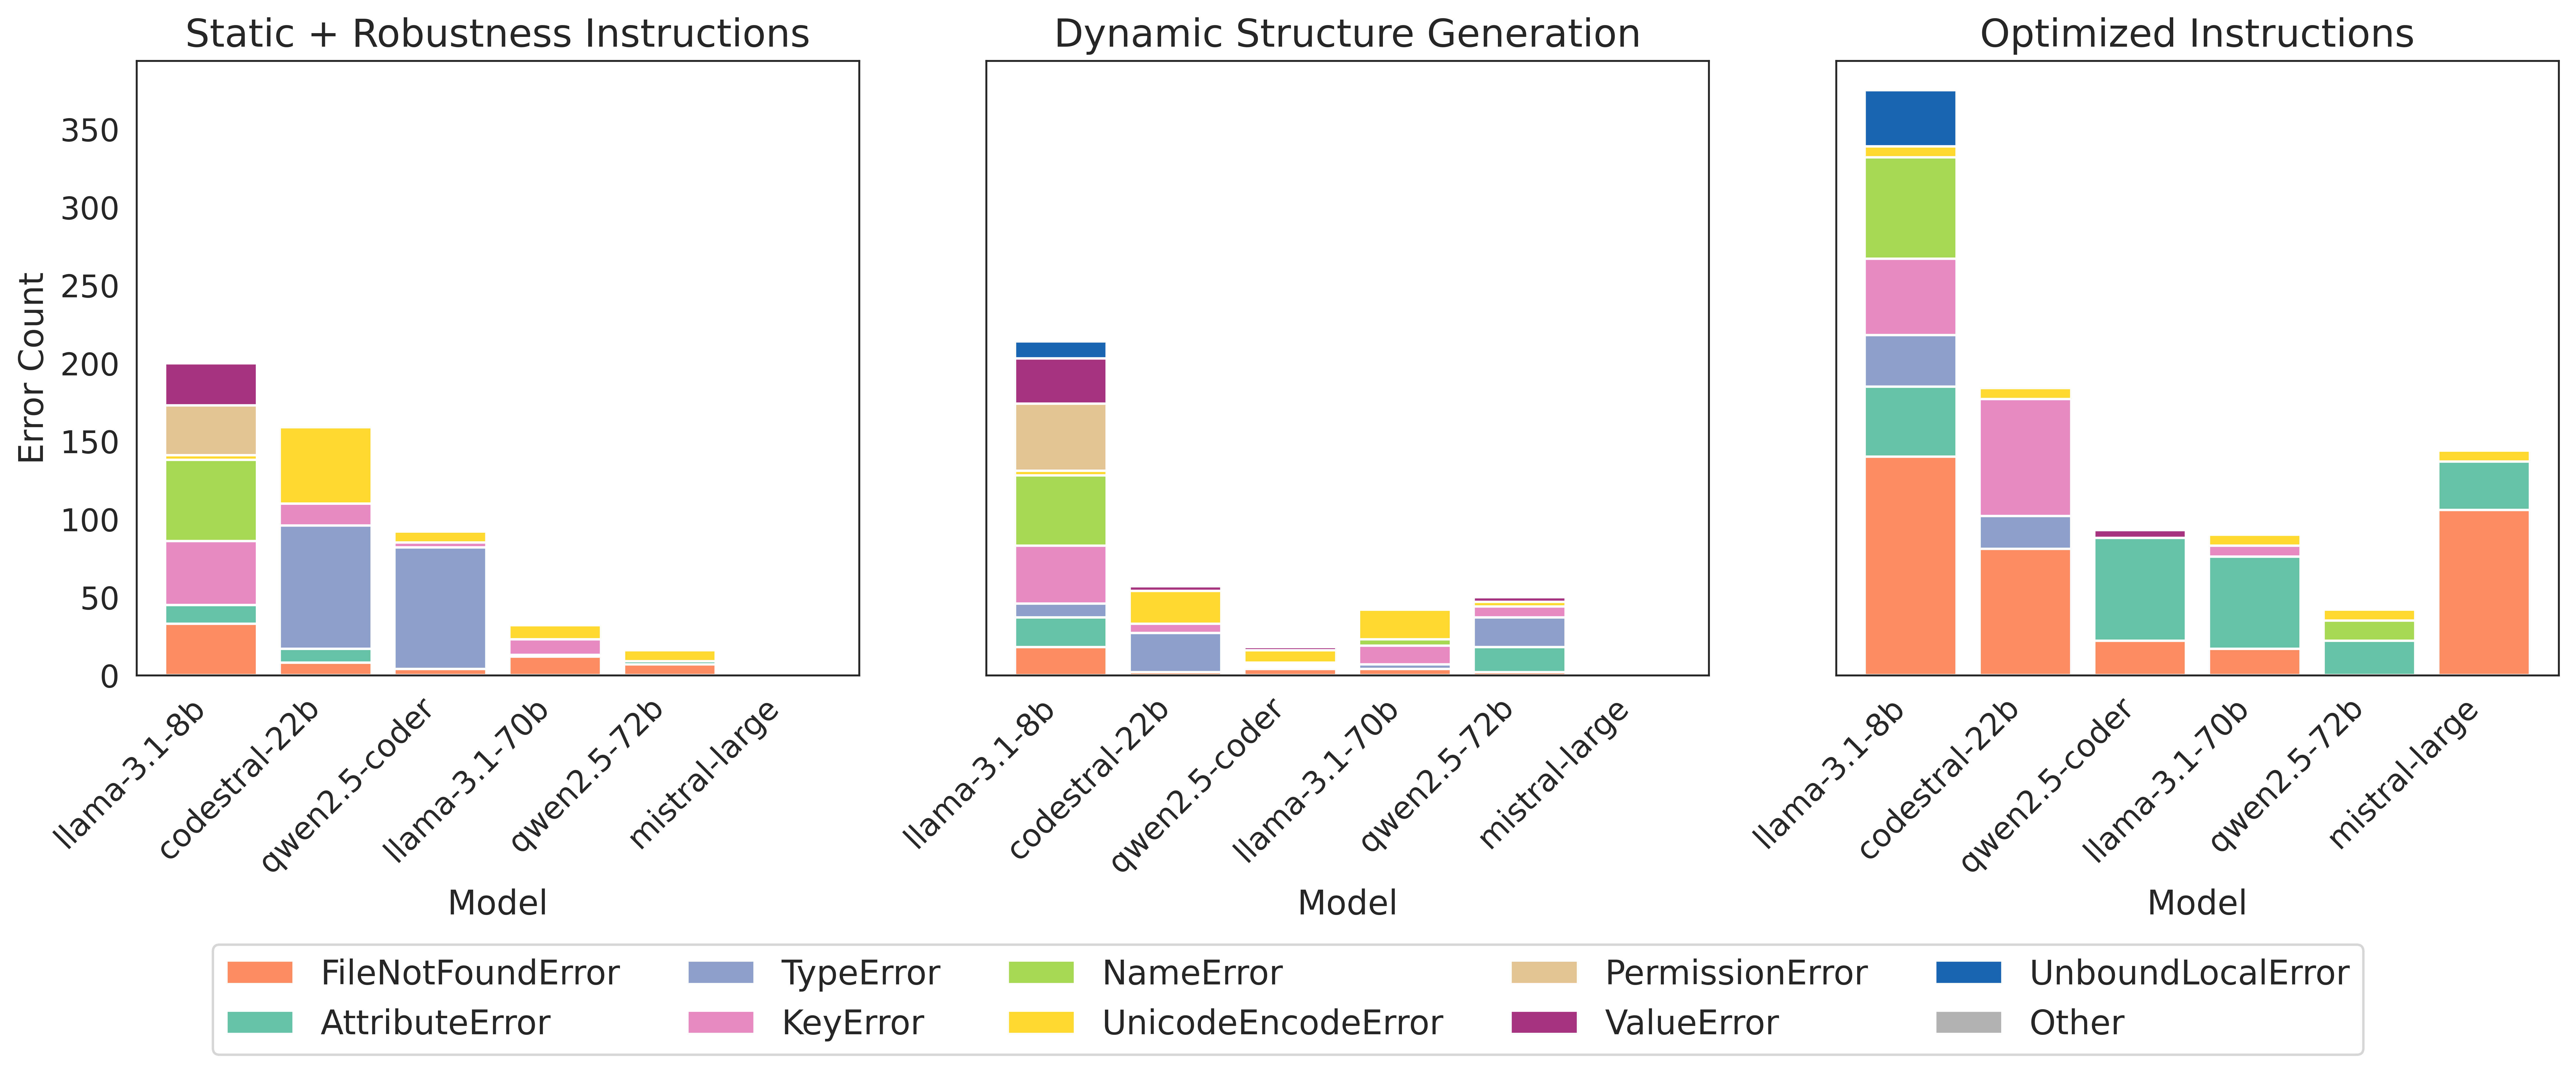
\includegraphics[width=\linewidth]{img/Results/Second Experimental Phase/Error Type Distribution per Model.png}
    \caption[Error type distribution]{\textbf{Error type distribution}. The stacked bar charts illustrate the frequency of the nine most common error types encountered for each model, grouped by experiment. Only the top 9 most frequent error types are shown explicitly, while all other less frequent errors are aggregated under “Other”.}
    \label{fig:error_distribution_second}
\end{figure}

Under the optimized instructions, the models are more likely to produce a FileNotFoundError compared to the robustness instructions and dynamic generation experiment (see Figure~\ref{fig:error_distribution_second}). This is particularly interesting, as the instructions in this experiment explicitly define the relevant file paths. The models most affected by this error in the third experiment are llama-3.1-8b, codestral-22b, and mistral-large. These results somewhat mirror the high failure rate observed for response outcomes on DDPs with missing data (see Figure~\ref{fig:outcome_distribution_nodata_second}), suggesting that these models do not implement sufficient measures to handle missing data. Another frequent error in this experiment is the AttributeError, indicating that the dictionary-related issues identified earlier are primarily focused here as well.

The models in the first two setups appear to be less prone to errors overall compared to the third experiment. During these first two experiments, only llama-3.1-8b occasionally struggles with FileNotFoundError. It is the most error-prone model in this phase, struggling with Python syntax issues and properly initializing or referencing objects. The rest of the models show a large variety in the types of errors produced. For example, in the first experiment, codestral-22b and qwen2.5-coder struggle with misidentifying the type of the processed object and improperly handling the data structures. In the second experiment, it is observed that the distributions of error types among the remaining models are much smaller. Among the aforementioned errors, we also observe a high frequency of UnicodeEncodeError, indicating that the models struggle with handling diverse content in some DDP data, likely special German letters or other symbols like emojis.

\begin{figure}[!b]
    \centering
    
\includegraphics[width=\linewidth]{img/Results/Second Experimental Phase/Error Trend Over Attempts.png}
    \caption[Error frequency trends over successive attempts]{\textbf{Error frequency trends over successive attempts}. The trend of error counts across multiple attempt numbers for each model, separated by experimental setup.}
    \label{fig:error_trends_second}
\end{figure}

Providing the structural context directly in the prompts is also more effective in enabling the models to fix their errors during retries. As shown in Figure~\ref{fig:error_trends_second}, across the experiments, models tend to resolve issues more efficiently within their first three attempts. In the first experiment, llama-3.1-70b and qwen2.5-72b typically correct their errors entirely by the second attempt. While other models also reduce their errors with each attempt, they generally reach a certain threshold where no further improvements occur. For these models, if an error is not resolved by the third or fourth attempt, it is more likely to persist until the response ultimately fails.

In the second experiment, qwen2.5-coder and llama-3.1-70b emerge as the most effective models in eliminating their errors entirely. Under this setup, the models generally demonstrate the highest efficiency in resolving generation issues with each successive attempt, with most achieving very low error rates in later attempts. Notably, even llama-3.1-8b performs considerably better under dynamic generation, showing a substantial error reduction, particularly between the first and third attempts. In this configuration, codestral-22b slightly outperforms qwen2.5-72b in error correction, even if by a very small margin. In the final experiment, however, qwen2.5-72b once again manages to resolve all its errors by the third attempt. In this setup, most models demonstrate high efficiency in fixing runtime errors by the third attempt, but then reach a stalemate. Beyond this point, they are generally unable to make substantial improvements to their generated code, with error rates either remaining stable or decreasing only marginally.

\subsection{Generated Code Analysis}

\paragraph{Raw and Halstead Metrics}\mbox{}\\

\begin{figure}[!b]
    \centering
    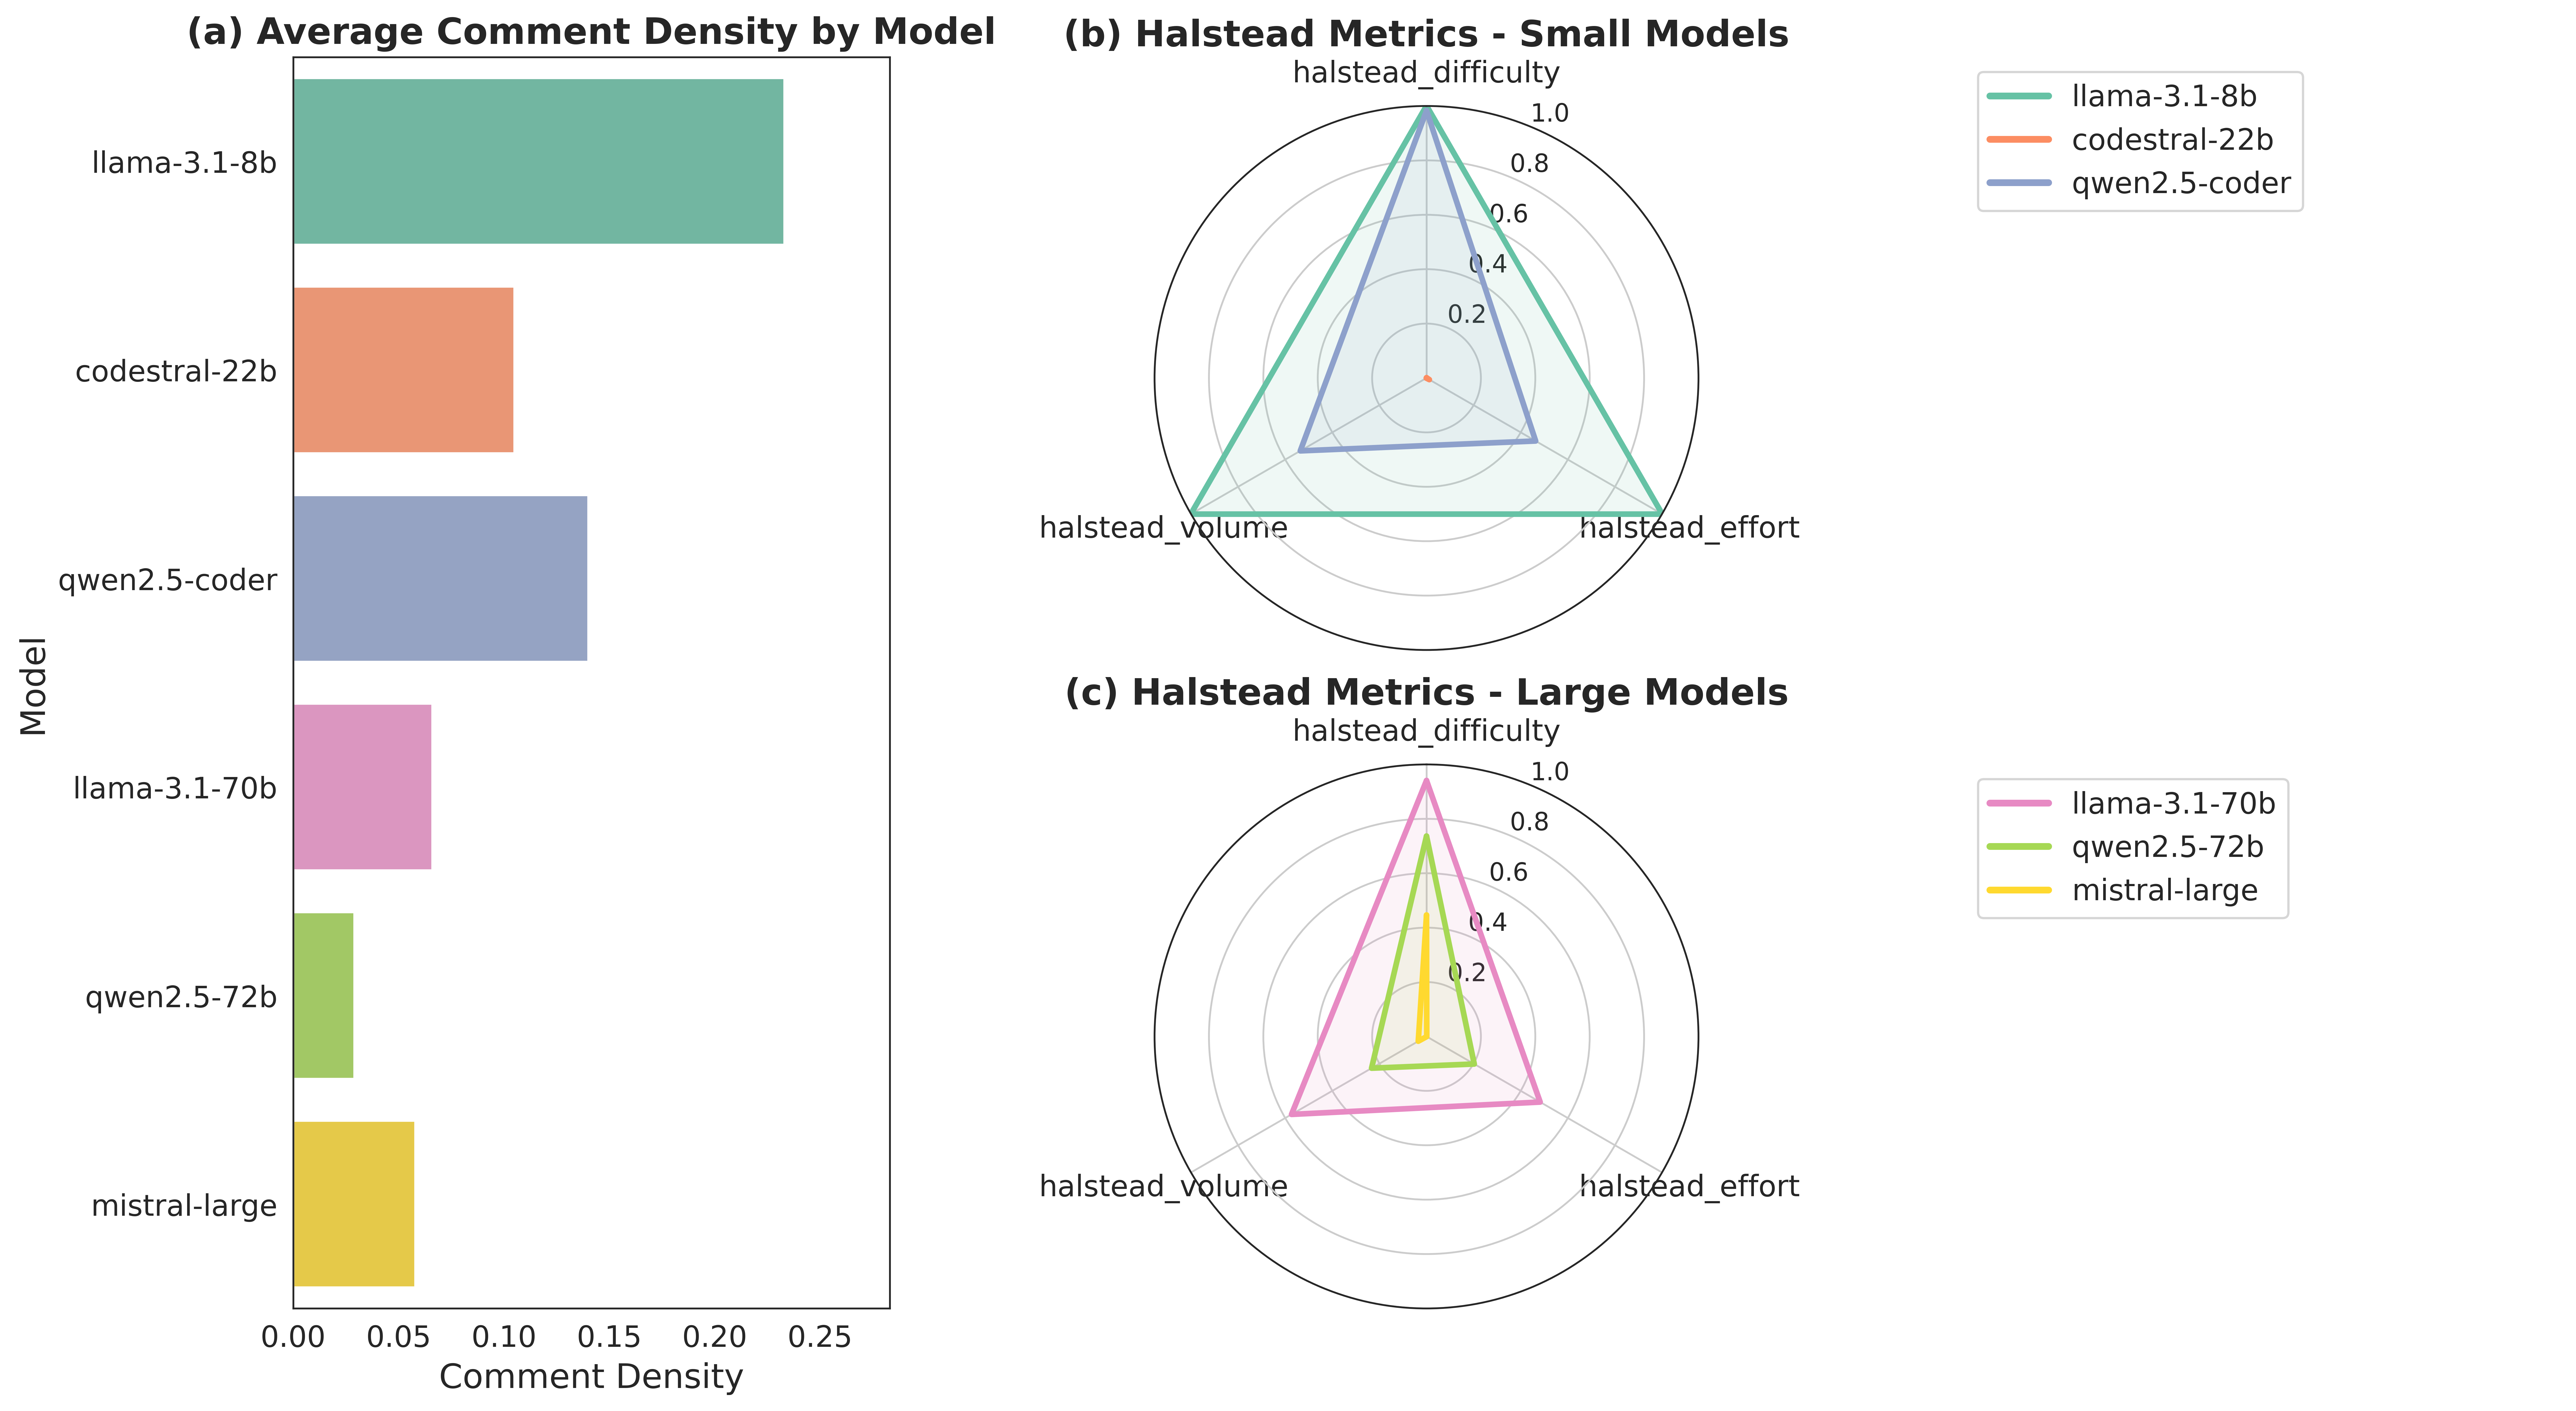
\includegraphics[width=\linewidth]{img/Results/Second Experimental Phase/Comment_Density_and_Halstead_Radar.png}
    \caption[Comment density and Halstead metrics across models]{\textbf{Comment density and Halstead metrics across models}. The bar plot (a) shows the average proportion of comments in generated code by each model. The radar charts present normalized Halstead metrics for small (b) and large (c) models, grouped by their size.}
    \label{fig:comment_density_and_halstead_second}
\end{figure}

\noindent In this experimental phase, the smaller models tend to include more comments in their code than the larger models (see Figure~\ref{fig:comment_density_and_halstead_second}). Llama-3.1-8b remains the model most likely to explain script lines, with 23.3\% of its generated code consisting of comments. A notable drop is seen with codestral-22b, which writes roughly one comment line for every ten lines of code, slightly less than qwen2.5-coder, which has a comment density of 14\%. An even sharper decrease occurs among the larger models, where the most accurate model, qwen2.5-72b, has a comment density of only about 3\%. This low density suggests that it may be documenting only key functions very briefly or that it prioritizes functionality over documentation.

In terms of Halstead metrics, codestral-22b retains its position as the model with the lowest overall values, producing very short code with a minimal number of operators and operands. In contrast, llama-3.1-8b has the highest difficulty, effort, and volume, suggesting either highly repetitive patterns or high complexity features in its solution. Under this prompt-based setup, qwen2.5-coder also produces code of notable difficulty, paired with moderate effort and volume, indicating a tendency toward compact but complex solutions. 

Among the larger models, we observe a bias toward difficulty as the dominant metric (see Figure~\ref{fig:comment_density_and_halstead_second}). Here, llama-3.1-70b emerges as the most complex, closely resembling qwen2.5-coder's generative habits. Excluding difficulty, mistral-large closely aligns with codestral-22b in both effort and volume, producing minimalistic code. Meanwhile, qwen2.5-72b combines very low effort and volume with relatively high difficulty, indicating a tendency for short code that may be technically demanding to follow. For both this model and mistral-large, the low volume likely contributes to their low documentation density, as there is simply less code to annotate.

\paragraph{Cyclomatic Complexity}\mbox{}\\

\begin{figure}[ht]
    \centering
    \includegraphics[width=\linewidth]{img/Results/Second Experimental Phase/Cyc_LOC_correlation.png}
    \caption[]{\textbf{Relationship between lines of code and cyclomatic complexity}. Scatter plots illustrating the relationship between source code size and total cyclomatic complexity for small and large models across the experiments. Regression lines (dashed) highlight overall trends, while $R^2$ values indicate the proportion of variance in cyclomatic complexity explained by LOC.}
    \label{fig:cyc_loc_correlation_second}
\end{figure}

\noindent The smaller models show moderate to high coefficients of determination in this experimental phase as well. As seen in Figure~\ref{fig:cyc_loc_correlation_second}, only llama-3.1-8b produces notable outliers across the first two experiments, reaching its peak cyclomatic complexity in the second experiment. Interestingly, this behavior is absent in the third experiment, suggesting that the optimized instructions guided the model toward more consistent structural patterns.

In this prompt-based setup, during the first two experiments, we observe a relatively strong correlation ($R^2=0.54$) for the smaller models under the robustness instructions and for the larger models in the dynamic structure generation setup. In the first experimental phase (see Figure~\ref{fig:cyc_loc_correlation}), the only case where larger models come close to a strong correlation also occurs in the dynamic generation setup. The absence of mistral-large in this configuration may have reduced structural variety and thus strengthened the observed relationship. Regardless, in both of these cases, longer code tends to come with proportionally higher cyclomatic complexity, suggesting a consistent scaling pattern between size and logical branching.

Surprisingly, the strongest relationship appears in the optimized instructions experiment for the smaller models, reaching an $R^2$ value of 0.60. This indicates that, under these instructions, the models often generate code that is structurally similar in terms of size and branching logic. This effect, however, is not observed among the larger models.

\begin{figure}[ht]
    \centering
    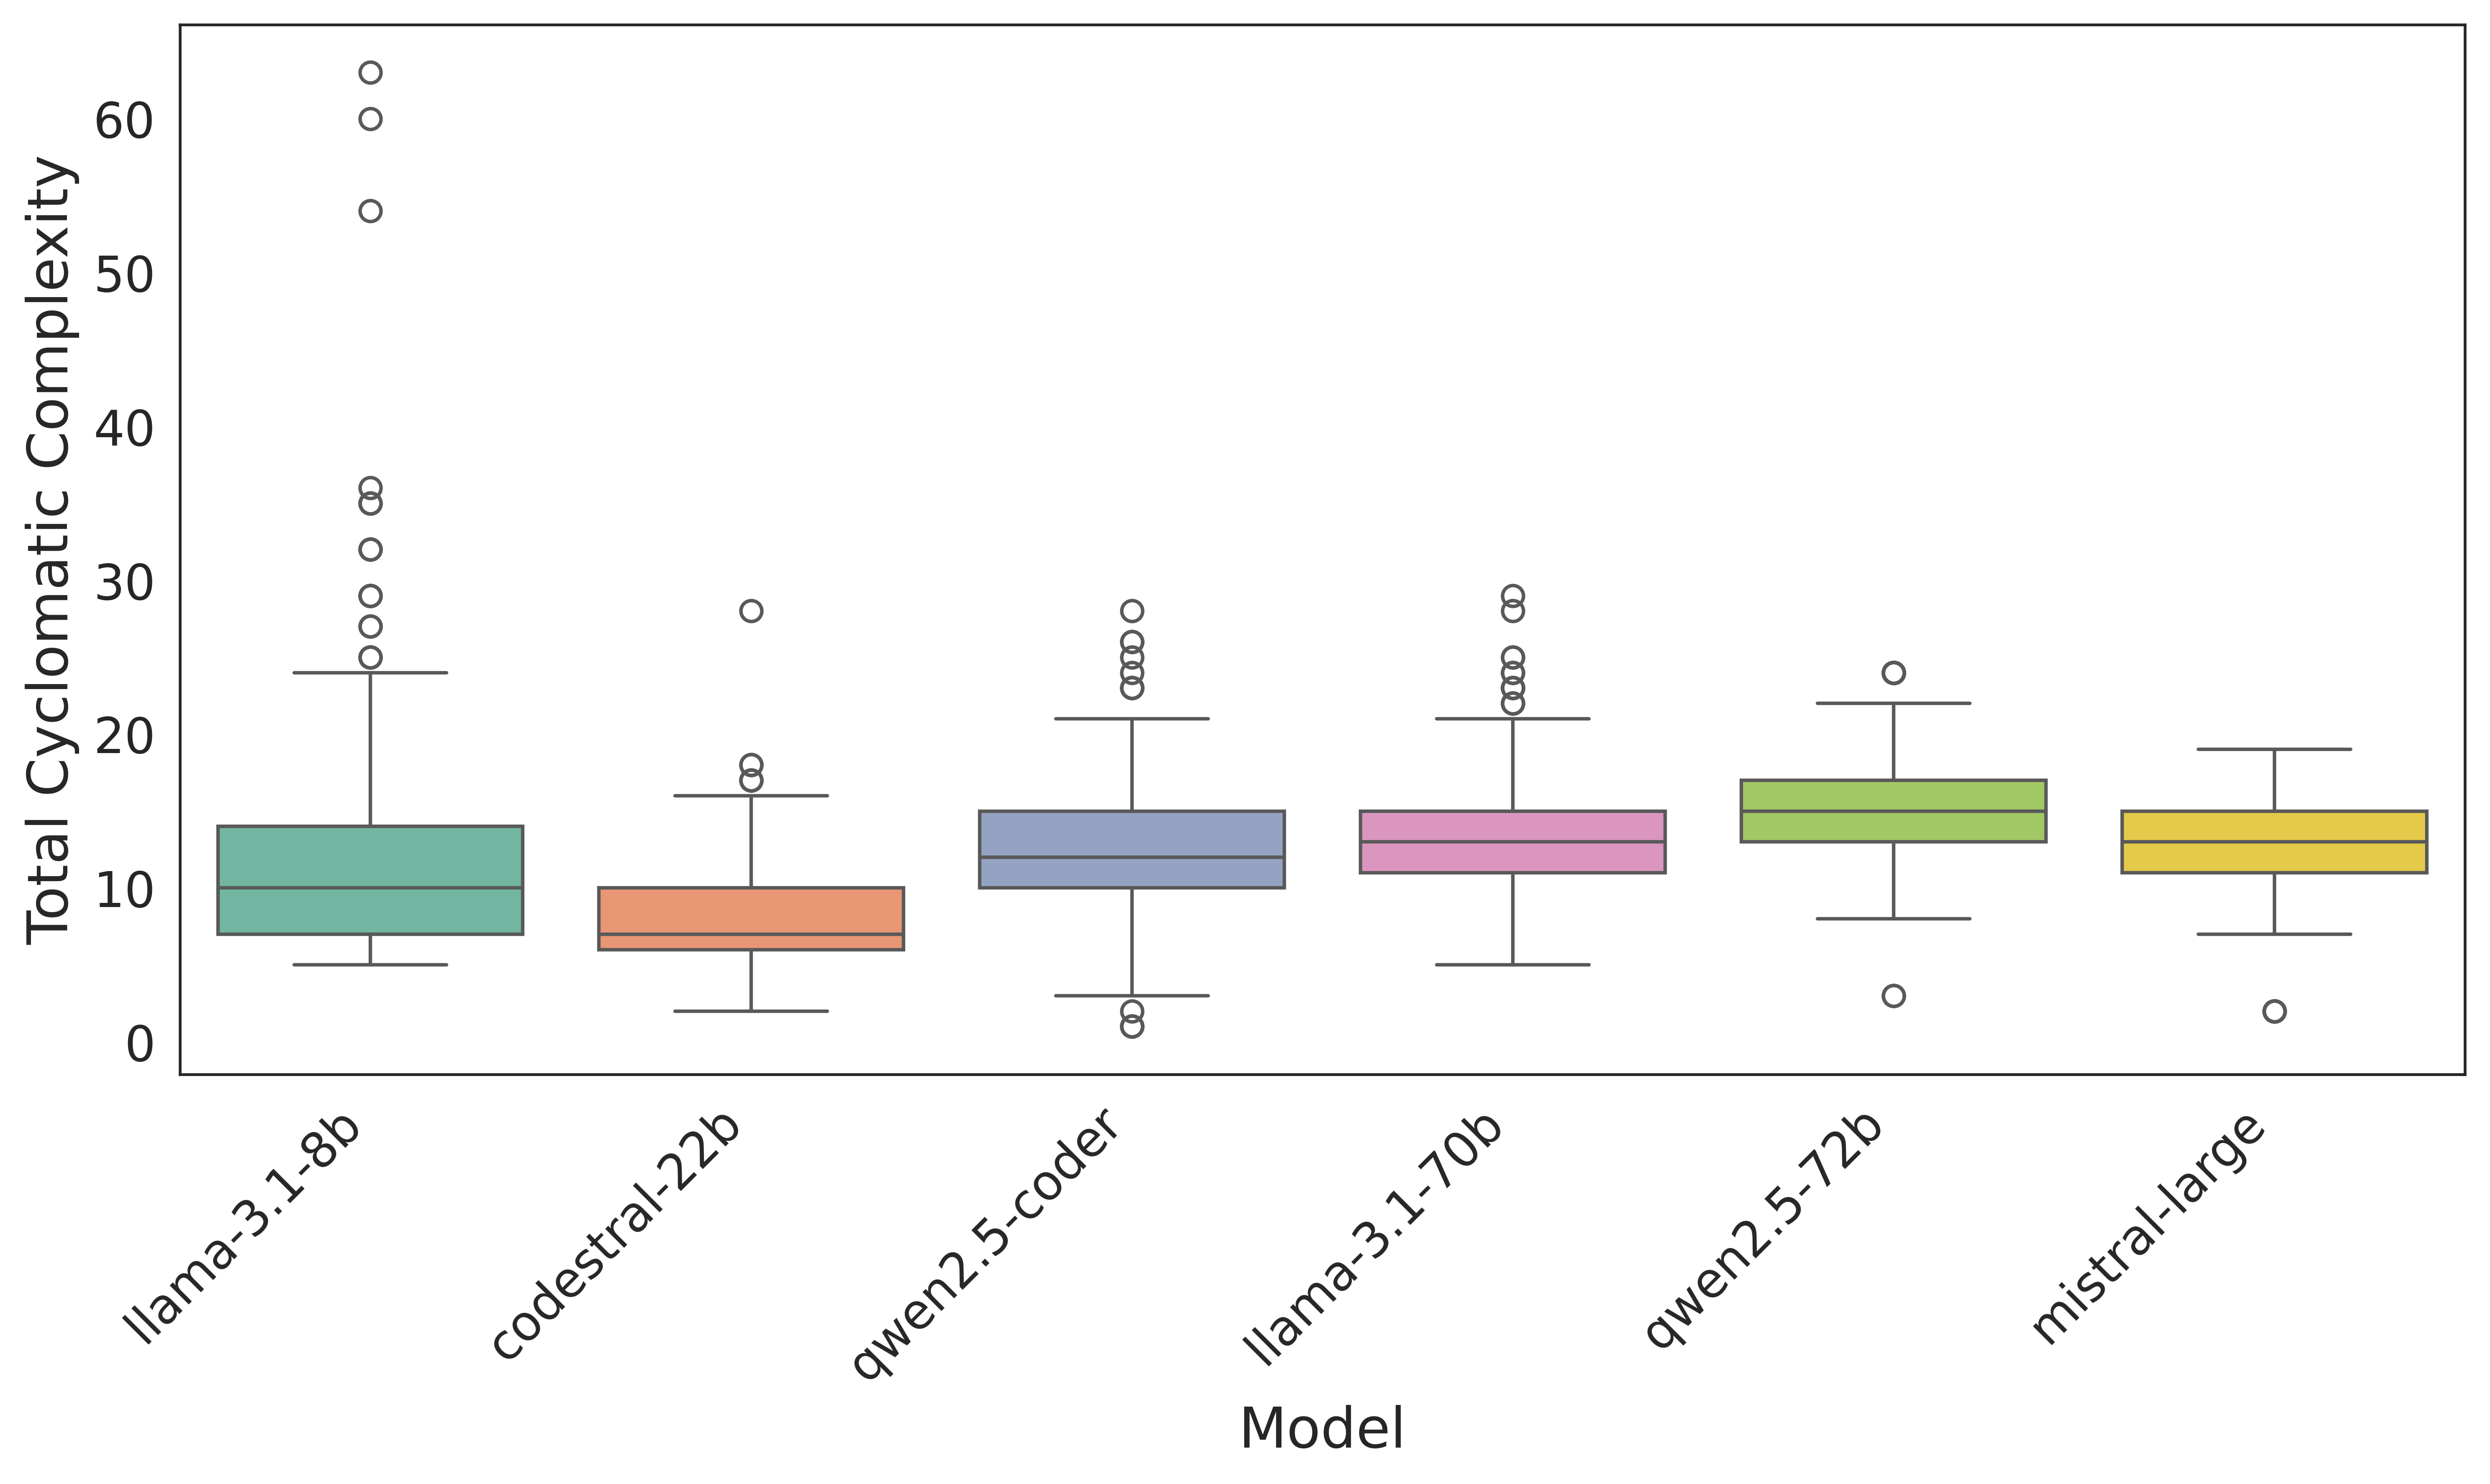
\includegraphics[width=0.65\linewidth]{img/Results/Second Experimental Phase/Cyclomatic Complexity Distribution per Model.png}
    \caption[Cyclomatic complexity distribution]{\textbf{Cyclomatic complexity distribution}. Boxplot showing the distribution of total cyclomatic complexity values for each evaluated model, aggregated across all experiments.}
    \label{fig:cyc_complexity_second}
\end{figure}

Again, the outliers in llama-3.1-8b's generated code are particularly highlighted in Figure~\ref{fig:cyc_complexity_second}, emphasizing this model's unpredictability. In this phase, most models exhibit a more balanced distribution of cyclomatic complexity. Aside from llama-3.1-8b, most models' box plots are relatively compact, indicating limited variability in the complexity of their outputs. Codestral-22b has the lowest mean, consistently producing simpler code with fewer decision points. In contrast, qwen2.5-72b shows the highest mean complexity, combined with relatively low variability, indicating that its outputs regularly contain more branching logic. Larger models generally generate code with higher average complexity than smaller models, which may contribute to their overall better performance and significantly higher accuracy.

\paragraph{Maintainability Index}\mbox{}\\

\noindent From an individual model perspective, in the first two experiments, llama-3.1-8b consistently achieves high maintainability scores, suggesting that its outputs are generally easier to interpret, an interesting contrast to its relatively high and erratic cyclomatic complexity values. Codestral-22b, which is typically in the mid range in terms of maintainability, experiences a substantial boost under the optimized instructions setup, reaching the highest values and mean across the entire experimental phase. The remaining models display stable, moderate performance, with larger models tending to score lower than the smaller ones. Notably, qwen2.5-72b records the lowest maintainability index values in every experiment. This trend may indicate that higher-accuracy code can be more difficult to maintain and understand, potentially due to reduced readability.

The prolific behavior observed in the first phase (see Figure~\ref{fig:MI_distribution}) appears to persist in this one as well (see Figure~\ref{fig:MI_distribution_second}). However, the profiles here show subtle differences and do not mirror the first phase's perfectly. This observation suggests that, although these models exhibit inherent tendencies and biases in code generation that are not greatly altered by the general prompt instructions, their behavior is notably influenced by how the structural context is provided to them.

\begin{figure}[h]
    \centering
    
\includegraphics[width=\linewidth]{img/Results/Second Experimental Phase/Maintainability Index per Model.png}
    \caption[Maintainability index distribution across experiments]{\textbf{Maintainability index distribution across experiments}. Boxplots showing the distribution of maintainability index scores for each model across the three experimental setups.}
    \label{fig:MI_distribution_second}
\end{figure}

\chapter{Discussion} \label{chap:discussion}

In this chapter, we present the overall results of our experiments and interpret the main findings. The full set of these results, along with the associated code, can be accessed in our public repository\footnote{\url{https://github.com/miger-shkrepa/adaptive-donated-data-analysis}}. We also provide alternative perspectives on these results and examine underlying factors that may have influenced the performance of the selected models. Finally, we discuss the limitations encountered in this study, which lay the groundwork for potential directions in future research.

\section{Interpretation of Results}

Below, we interpret the experimental results presented in Chapter~\ref{chap:results} and use them to answer the research questions outlined in Section~\ref{research_objective}.

\subsection{RAG-Based Querying Performance}

Our experimental results indicate that the current performance of RAG for analyzing DDPs requires significant enhancements before it can be considered for deployment. The experiments overall yield inferior results, to the extent that no setup involving RAG is advisable under the current state. By analyzing the most likely error types and the models' unsuccessful attempts to address them (see Subsection~\ref{RAG_error_analysis}), faulty path generation is highlighted as the primary contributor to this setup's weaknesses. In most experimental instances, the generated code attempts to access files through non-existent or incorrect paths, often due to the model removing some levels of the folder hierarchy when constructing them. We speculate that this behavior might be a direct result of the retrieval-related imperfections discussed in Section~\ref{rag_weaknesses}, particularly those linked to long-distance information dependencies (refer to Table~\ref{tab:rag_error_types_adapted}). This error occurs when large spans of text separate question-related and answer-related information and is a common issue when embedding longer documents~\cite{Chen_Lin_Han_Sun_2024}. Given the size and complexity of the Instagram data structure, this would explain the path segmentation. Some folders in this structure contain several JSON files, and many of these files in turn store multiple JSON objects that they keep track of. As the hierarchy deepens, the distance between an answer-relevant JSON object and its parent directories grows longer, raising the likelihood that one or more folders in the hierarchy are dropped during model reasoning, leading to systematic segmentation errors.

\subsection{Direct Contextual Prompting Performance}

The first two experiments of the prompt-based experimental phase mirror the last two experiments of the RAG-based phase, differing only in how the DDP structure is provided. This makes them a strong basis for comparing the two approaches and answering \textbf{RQ3}. Overall, providing the complete structure directly in the prompt proves more efficient and accurate than relying on an external knowledge base. In these experiments, models consistently achieve higher accuracy. They capture and use information more effectively as they are able to answer a wider range of the designed data queries. In addition, the models in this setup are less prone to runtime errors and more successful in correcting coding mistakes through retries. Taken together, these results address \textbf{RQ3} and make the choice clear: a direct prompt-based approach yields superior outcomes compared to an RAG incorporation.

However, caution is warranted. The full scope of a DDP may exceed some models' context windows for prompt injection, as demonstrated by the exclusion of mistral-large due to this limitation. Moreover, despite the relative improvement over RAG, neither approach achieves results that could be considered satisfactory. Each suffers from trade-offs and shortcomings that would prevent practical deployment without further enhancements to the underlying models or the consideration of other LLMs.

These shortcomings motivate the design of the final experiment, in which optimized instructions are introduced to guide the models more effectively. As such, to address \textbf{RQ4}, when provided with detailed structural information and explicit indications of which data to target, the models achieve their best performance. The overall results answer \textbf{RQ1} and \textbf{RQ2}, demonstrating that while models operating under a basic setting often misinterpret the DDP structure and yield low to moderate performance, additional guidance can substantially improve outcomes, in some cases approaching near-perfect results. Nevertheless, this does not imply that the models are free from data processing or extraction errors, nor from issues of faulty code generation. In practice, retries are often required to correct such errors, or further improvements to the models themselves may be necessary.

\subsection{Can Adaptive Code Generation Truly Eliminate Manual Intervention?}

It is important to note that even the final experiment reveals important limitations in this study. The primary focus of this research is to explore the feasibility of adaptive code generation. Specifically, whether researchers can reduce the need for manually updating data donation tools as DDP structures evolve by leveraging LLMs. While some models under the optimized instructions achieve near-perfect results, this success is contingent on multiple, highly detailed instructions. Consequently, if the data structure were to change, these instructions would also need to be revised. In this sense, the process comes full circle as the effort to improve performance and eliminate errors reintroduces the need for manual intervention. This observation highlights both the potential and the current limitations of LLMs in the domain of analyzing donated data. They can provide significant support in automating and streamlining the process. However, their ability to independently interpret complex structures and accurately map queries to the relevant parts of the DDP structure remains insufficient, at least for the models evaluated in this study.

\section{In Defense of the LLMs}

The optimized instructions are designed to address three key areas of weakness observed in the models. The first set of instructions involves providing the explicit path to the files relevant to a given query. However, even with these paths, the LLMs often struggle to interpret them correctly (see Figure~\ref{fig:answer_type_classification_second}). 

Hallucination is a common issue in LLMs, and the deep and intricate structure of the Instagram DDP appears to amplify it. Concept confusion (see Table~\ref{tab:rag_error_types_adapted}) is especially likely to occur. For example, when asked to identify the topics of interest Instagram records for a user, the correct answer resides in the file \emph{recommended\_topics.json}, with the keyword topic serving as the connection. Some models, however, incorrectly look in \emph{locations\_of\_interest.json}, latching onto the shared keyword “interest”. Similar naming conventions are used throughout the dataset, enhancing the confusion. To mitigate this, the final experiment restricts the input to only the relevant JSON object structures.

However, these two instructions alone are not enough for a consistently strong performance, as the models still generate inaccurate responses. Upon closer examination, the over-complexity of the Instagram DDP also becomes apparent within the content of the JSON files themselves. For instance, the JSON object recorded in \emph{recommend\_topics.json} is structured as:
\begin{lstlisting}[language=Python]
"topics_your_topics": [
    {
        "media_map_data": {},
        "string_map_data": {
            "Name": {
                "href": "str",
                "timestamp": "int",
                "value": "str"
            }
        },
        "title": "str"
    }]
\end{lstlisting}
The design of this structure introduces object-level ambiguity, as the models have to choose whether to extract the response data from the \emph{Name.value} field or the \emph{title} property. In this example, both properties appear to contain the correct answer data, but only one is the right choice. Similar ambiguities can be observed across other object structures in the Instagram dataset.

Thus, the poor performance cannot be attributed solely to the LLMs but also to the inherent complexity of the Instagram DDP structure. When conducting this research, the Instagram-issued DDP was recognized as an ideal candidate for this feasibility evaluation due to its scale and intricate design. However, these complexity qualities may have hindered the models' performance. 

\section{Limitations}

The evaluation framework of this thesis relies on sensitive data derived from individual Instagram DDPs. Such datasets are not easily found as standardized public benchmarks, so the packages used in this study are collected directly from various individuals. This process raises ethical concerns, as not all individuals may feel comfortable sharing their personal data. Even when they do, this does not imply consent to sharing all aspects of it. To respect these concerns and in accordance with GDPR, the datasets used in this study, along with the generated ground truth CSV files, will not be published or made available for external review.

It is important to note that the ground truths used in this study are not manually established but generated with the assistance of larger LLMs. After a collaborative analysis of the structure with LLMs, examining their reasoning, and how they mapped each data query to particular JSON objects, we adopt these outputs as the ground truths. However, this does not guarantee that the resulting CSVs represent the definitive ground truths for every question. Instead, they reflect the most plausible interpretations for some of them. Another limitation concerns the nature of the evaluation questions. Due to the experimental design, the asked questions are restricted to quantitative queries. As such, the evaluation captures measurable information but does not extend to qualitative insights or interpretations of the data.

Employing LLMs involves considerable computational costs and resource constraints. In this study, the models are accessed through API services, which introduce limitations of their own. For a single experiment, between 780 and 936 API requests are required at a minimum, not including error fixing retries (up to five per request), meaning the actual number could be substantially higher. As a result, API rate limits can be exceeded multiple times, causing delays until further access is allowed. Moreover, depending on the service and model, response times may vary significantly. Popular models are often slower, and in some cases, almost inaccessible. For example, during the course of this study, the llama-3.1-70b model repeatedly timed out due to long response times, which required switching to an alternative API service.

Finally, this study evaluates DDPs issued by a single data controller. While this decision provides a controlled environment for experimentation, it also limits the diversity of the datasets. As a result, the findings are inherently biased toward the structure and characteristics of Instagram's DDPs. As previously discussed, these characteristics introduce challenges that negatively impact model capabilities as well. Since different data controllers issue DDPs with varying levels of complexity, scale, and interpretability, the performance results observed here may not generalize across other platforms.

\section{Future Research}

The previously discussed limitations provide the groundwork for several possible directions in future research. First, a more diverse set of DDPs from different data controllers, with varying levels of depth and complexity, can be explored. This would allow for an assessment of model performance on datasets that may be less complex than the one explored in this thesis. Another approach would be to investigate the difficulty threshold at which models begin to struggle. By gradually moving from simpler structures toward increasingly complex ones, a more nuanced understanding of how structural difficulty affects accuracy could be offered.

Another direction would be to explore a broader range of LLMs. While this study includes models of varying sizes and from different developers, future work could incorporate models specifically fine-tuned for data analysis or task-focused code generation. Researchers might also experiment with training custom models tailored to the DDP structure that they are focusing their research on. 

The RAG process could be extended by incorporating additional supporting documents. For instance, guidelines on how to approach the task, coding best practices, or other domain-relevant resources could be passed alongside the data structure. Such additions might enhance the models' reasoning process and reduce common sources of error, ultimately improving RAG performance.

\chapter{Conclusion} \label{chap:conclusion}

After conducting a thorough experimental framework, this thesis provides insights into the expectations and feasibility of employing LLMs for adaptive code generation. Although RAG has revolutionized model responses by integrating external knowledge to reduce hallucinations and improve accuracy, it does not deliver satisfactory results in this study. The models frequently generate faulty paths or misinterpret the provided context. A prompt-based setup performs better in comparison, but the results are still unsatisfactory, partly due to incorrect data extraction and processing methods. Upon closer examination, the poor performance observed in both setups appears closely tied to the over-complex structure of Instagram's DDPs, which enhances hallucination tendencies and is inherently difficult for the models to interpret.

In an effort to improve this performance, we experiment with providing the models with detailed instructions on how to handle the data and navigate Instagram's complex structures. This approach significantly enhances performance, yet it also highlights how these highly detailed and manual instructions are crucial for the models to yield better results. The objective of this research is to investigate the feasibility of removing the need for researchers to manually update tools in response to DDP structural changes. Our experiments show that, while LLMs show potential in adapting to structural changes in donated data packages, their effectiveness still depends on the very manual interventions this research aims to reduce. At the same time, a DDP researcher without programming skills but with knowledge of how the donated data is structured can still use LLMs to automate processes by having them generate code. This finding underscores both the current limitations of LLMs in this domain and lays down possible future directions for further research on this topic. 

Identifying the strengths, weaknesses, and potential of these models in adapting to structural changes in donated data packages helps in setting realistic expectations for employing them in the domain of this task, but also illustrates how much room there is for improvement.

\sloppy
\addcontentsline{toc}{chapter}{Bibliography}
\printbibliography

\appendix

\chapter{Methodology}

\section{Prompt Structure and Design}

Figure~\ref{fig:query_instructions} shows the base prompt used in this study, which defines the code generation rules.

\begin{figure}[h]
    \centering
    \fbox{%
        \begin{minipage}{0.95\linewidth}
        This is the tree structure of a directory containing user data. This directory consists of several nested folders, JSON files with unique structures, and other types of files. You will be asked to generate Python scripts for unique queries based on this data. The generated code must follow these rules:

        \begin{enumerate}[noitemsep, topsep=0pt]
            \item The code must be designed such that the file input corresponds to the main folder, which is the first and top-level object in the directory structure.
            \item The variable referring to the file input must be declared in a single line. For example: \texttt{root\_dir = "value"}.
            \item This variable must be named \texttt{root\_dir}.
            \item Use only standard Python libraries; avoid external dependencies such as \texttt{pandas}, \texttt{numpy}, etc.
            \item The code must include proper error handling.
            \item Errors must be raised as proper Python exceptions (e.g., FileNotFoundError, ValueError), with messages beginning with "Error: " followed by the reason for failure.
            \item Error raising must follow this format: \newline
            \texttt{raise FileNotFoundError("FileNotFoundError: The root directory does not exist.")}
            \item \{query-specific instructions\}
            \item Save the resulting CSV file at \texttt{'query\_responses/results.csv'}. This path indicates where the output file should be stored and should not be considered part of the input data directory.
        \end{enumerate}
        
        Based on this directory structure, please create a Python script that answers the following query: \{query\}
        \end{minipage}
    }
    \caption[Prompt instructions for code generation]{\textbf{Prompt instructions for code generation}. Contextual information and rules to ensure that the generated Python code adheres to the automated evaluation schema. Here, the variables enclosed in curly brackets denote values dynamically specific to the pipeline iteration.}
    \label{fig:query_instructions}
\end{figure}

\section{Data Queries and Response Structure}

\subsection{Questions Designed for Model Evaluation}

Figure~\ref{fig:used_queries} shows the complete list of queries used in evaluating the LLMs.

\begin{figure}[h]
    \centering
    \fbox{%
        \begin{minipage}{0.95\linewidth}
        \begin{enumerate}
            \item What topics does Instagram determine to be of interest for a user?
            \item How often does a user see advertisements and about which topics (from which companies)?
            \item How often do people see posts(daily and weekly)?
            \item Which companies have access to your Instagram activity or information?
            \item Which devices has the user logged in from and when?
            \item What Instagram account changes (e.g., name, phone, email) has the user made over time?
            \item Whose stories does the user tend to engage with most often?
            \item Which accounts has the user interacted with most often through post likes, story likes and comments(Top 20)?
            \item Which profiles does the user follow that do not follow him back?
            \item How often does the user view content (including both posts and videos) and from which accounts?
            \item Which accounts has the user viewed posts from but not liked them?
            \item How many messages does the user send per week?
        \end{enumerate}
        \end{minipage}
    }
    \caption[Data queries used in the experiment]{\textbf{Data queries used in the experiment}. A complete list of the natural language queries used to evaluate the models across various features of Instagram's DDPs.}
    \label{fig:used_queries}
\end{figure}

\newpage

\subsection{Structured Output Instructions}

To ensure that all models' responses are compatible with a shared evaluation methodology, specific query instructions are designed for each question (see Figure~\ref{fig:query_response_instructions}).

\begin{figure}[h]
    \centering
    \fbox{%
        \begin{minipage}{0.95\linewidth}
        \begin{enumerate}[noitemsep, topsep=0pt]
            \item The response must be a structured CSV file with one column: Topics of Interest.
            \item The response must be a structured CSV file with two columns: Company Name and Number of Ads Viewed.
            \item The response must be a structured CSV file with three columns: Date/Week, Posts Viewed and Type. The 'Type' column must contain either 'Daily' or 'Weekly' as values. The 'Date/Week' Column must follow the 'YYYY-MM-DD' format (e.g., 2025-01-18) for daily dates and the 'Week YYYY-WW' format (e.g., Week 2025-02) for weeks. The weekly value must be generated using strftime('\%Y-\%W'), where weeks start on Monday.
             \item The response must be a structured CSV file with one column: Company Name.
            \item The response must be a structured CSV file with two columns: Device ID and Login Time. The 'Login Time' column must follow the 'YYYY-MM-DD HH:MM:SS' format (e.g., 2025-01-21 12:46:26).
            \item The response must be a structured CSV file with three columns: Changed, New Value and Change Date. The 'Change Date' Column must follow the 'YYYY-MM-DD' format (e.g., 2025-01-18).
            \item The response must be a structured CSV file with two columns: User and Times Engaged.
            \item The response must be a structured CSV file with four columns: User, Post Likes, Story Likes and Comments.
            \item The response must be a structured CSV file with one column: Profile.
            \item The response must be a structured CSV file with three columns: Account,Post Views and Video Views.
            \item The response must be a structured CSV file with one column: Account.
            \item The response must be a structured CSV file with two columns: Week and Messages Sent. The 'Week' column must follow the 'Week YYYY-WW' format (e.g., Week 2025-02). The weekly value must be generated using strftime('\%Y-\%W'), where weeks start on Monday. Within the 'inbox' directory, each conversation is stored in its own subfolder. The folder names are anonymized or unique, so do not assume a fixed name like 'username\_placeholder'. In each subfolder, look for one or more message\_X.json files, where X is a sequential digit starting from 1 (e.g., message\_1.json, message\_2.json, ...). The files must be read in order, and there won't be gaps in numbering.
        \end{enumerate}
        \end{minipage}
    }
    \caption[Query response instructions]{\textbf{Query response instructions}. Outline of the required CSV output instructions. It specifies the expected column headers, acceptable value formats, and additional constraints particular to questions referring to temporal data or complex data structures.}
    \label{fig:query_response_instructions}
\end{figure}

\newpage

\section{Pipeline Overview}

\subsection{Structure Recorder Output}

Figure~\ref{fig:data_structure_snippet} shows an example snippet of the output of the structure recorder. The generated structure is saved as a formatted JSON string into a textual file.

\begin{figure}[H]
\begin{lstlisting}[language=Python]
{
    "ads_information": {
        "ads_and_topics": {
            "ads_viewed.json": {
                "type": "json",
                "structure": {
                    "impressions_history_ads_seen": [
                        {
                            "string_map_data": {
                                "Author": {
                                    "value": "str"
                                },
                                "Time": {
                                    "timestamp": "int"
                                }
                            }
                        },
                        {
                            "string_map_data": {
                                "Time": {
                                    "timestamp": "int"
                                }
                            }
                        }
                    ]
                }
            },
\end{lstlisting}
\caption[Example snippet of the generated data structure file]{\textbf{Example snippet of the generated data structure file}. The structure recorder captures the hierarchy of the DDP directory in JSON format. When encountering JSON files, their structure, including the objects and fields, is recorded as well while masking the values to ensure no sensitive data is included.}
\label{fig:data_structure_snippet}
\end{figure}

\end{document}  